% Options for packages loaded elsewhere
\PassOptionsToPackage{unicode}{hyperref}
\PassOptionsToPackage{hyphens}{url}
\documentclass[
  spanish,
  12pt,
]{article}
\usepackage{xcolor}
\usepackage[margin=2.5cm]{geometry}
\usepackage{amsmath,amssymb}
\setcounter{secnumdepth}{-\maxdimen} % remove section numbering
\usepackage{iftex}
\ifPDFTeX
  \usepackage[T1]{fontenc}
  \usepackage[utf8]{inputenc}
  \usepackage{textcomp} % provide euro and other symbols
\else % if luatex or xetex
  \usepackage{unicode-math} % this also loads fontspec
  \defaultfontfeatures{Scale=MatchLowercase}
  \defaultfontfeatures[\rmfamily]{Ligatures=TeX,Scale=1}
\fi
\usepackage{lmodern}
\ifPDFTeX\else
  % xetex/luatex font selection
\fi
% Use upquote if available, for straight quotes in verbatim environments
\IfFileExists{upquote.sty}{\usepackage{upquote}}{}
\IfFileExists{microtype.sty}{% use microtype if available
  \usepackage[]{microtype}
  \UseMicrotypeSet[protrusion]{basicmath} % disable protrusion for tt fonts
}{}
\makeatletter
\@ifundefined{KOMAClassName}{% if non-KOMA class
  \IfFileExists{parskip.sty}{%
    \usepackage{parskip}
  }{% else
    \setlength{\parindent}{0pt}
    \setlength{\parskip}{6pt plus 2pt minus 1pt}}
}{% if KOMA class
  \KOMAoptions{parskip=half}}
\makeatother
\usepackage{longtable,booktabs,array}
\usepackage{calc} % for calculating minipage widths
% Correct order of tables after \paragraph or \subparagraph
\usepackage{etoolbox}
\makeatletter
\patchcmd\longtable{\par}{\if@noskipsec\mbox{}\fi\par}{}{}
\makeatother
% Allow footnotes in longtable head/foot
\IfFileExists{footnotehyper.sty}{\usepackage{footnotehyper}}{\usepackage{footnote}}
\makesavenoteenv{longtable}
\usepackage{graphicx}
\makeatletter
\newsavebox\pandoc@box
\newcommand*\pandocbounded[1]{% scales image to fit in text height/width
  \sbox\pandoc@box{#1}%
  \Gscale@div\@tempa{\textheight}{\dimexpr\ht\pandoc@box+\dp\pandoc@box\relax}%
  \Gscale@div\@tempb{\linewidth}{\wd\pandoc@box}%
  \ifdim\@tempb\p@<\@tempa\p@\let\@tempa\@tempb\fi% select the smaller of both
  \ifdim\@tempa\p@<\p@\scalebox{\@tempa}{\usebox\pandoc@box}%
  \else\usebox{\pandoc@box}%
  \fi%
}
% Set default figure placement to htbp
\def\fps@figure{htbp}
\makeatother
% definitions for citeproc citations
\NewDocumentCommand\citeproctext{}{}
\NewDocumentCommand\citeproc{mm}{%
  \begingroup\def\citeproctext{#2}\cite{#1}\endgroup}
\makeatletter
 % allow citations to break across lines
 \let\@cite@ofmt\@firstofone
 % avoid brackets around text for \cite:
 \def\@biblabel#1{}
 \def\@cite#1#2{{#1\if@tempswa , #2\fi}}
\makeatother
\newlength{\cslhangindent}
\setlength{\cslhangindent}{1.5em}
\newlength{\csllabelwidth}
\setlength{\csllabelwidth}{3em}
\newenvironment{CSLReferences}[2] % #1 hanging-indent, #2 entry-spacing
 {\begin{list}{}{%
  \setlength{\itemindent}{0pt}
  \setlength{\leftmargin}{0pt}
  \setlength{\parsep}{0pt}
  % turn on hanging indent if param 1 is 1
  \ifodd #1
   \setlength{\leftmargin}{\cslhangindent}
   \setlength{\itemindent}{-1\cslhangindent}
  \fi
  % set entry spacing
  \setlength{\itemsep}{#2\baselineskip}}}
 {\end{list}}
\usepackage{calc}
\newcommand{\CSLBlock}[1]{\hfill\break\parbox[t]{\linewidth}{\strut\ignorespaces#1\strut}}
\newcommand{\CSLLeftMargin}[1]{\parbox[t]{\csllabelwidth}{\strut#1\strut}}
\newcommand{\CSLRightInline}[1]{\parbox[t]{\linewidth - \csllabelwidth}{\strut#1\strut}}
\newcommand{\CSLIndent}[1]{\hspace{\cslhangindent}#1}
\ifLuaTeX
\usepackage[bidi=basic,shorthands=off,]{babel}
\else
\usepackage[bidi=default,shorthands=off,]{babel}
\fi
\ifLuaTeX
  \usepackage{selnolig} % disable illegal ligatures
\fi
\setlength{\emergencystretch}{3em} % prevent overfull lines
\providecommand{\tightlist}{%
  \setlength{\itemsep}{0pt}\setlength{\parskip}{0pt}}
% Header LaTeX para controlar tamaño de imágenes Mermaid
% Limita TODAS las imágenes a max 75% del ancho de texto
\usepackage[export]{adjustbox}
\let\oldincludegraphics\includegraphics
\renewcommand{\includegraphics}[2][]{%
  \oldincludegraphics[max width=0.75\textwidth,center,#1]{#2}%
}
\usepackage{bookmark}
\IfFileExists{xurl.sty}{\usepackage{xurl}}{} % add URL line breaks if available
\urlstyle{same}
\hypersetup{
  pdflang={es},
  hidelinks,
  pdfcreator={LaTeX via pandoc}}

\author{}
\date{}

\begin{document}

\begin{titlepage}
    \centering
    \thispagestyle{empty}
    
    \vspace*{2cm}
    
    {\LARGE \textbf{Modelo de Optimización para la Planificación de Coproductos con Metaheurísticas en la Industria Avícola}}
    
    \vspace{3cm}
    
    {\large Daniel Andrés Castañeda Rodríguez}
    
    \vspace{3cm}
    
    
\includegraphics[width=16cm]{logo_utp.png}
    
    \vspace{3cm}
    
    {\normalsize Universidad Tecnológica de Pereira}
    
    \vspace{0.3cm}
    
    {\normalsize Maestría en Investigación de Operaciones y Estadística}
    
    \vspace{0.5cm}
    
    {\normalsize 2026}
    
\end{titlepage}

\newpage

\begin{titlepage}
    \centering
    \thispagestyle{empty}
    
    \vspace*{1cm}
    
    {\large \textbf{UNIVERSIDAD TECNOLÓGICA DE PEREIRA}}
    
    \vspace{0.3cm}
    
    {\normalsize Facultad de Ingeniería Industrial}
    
    \vspace{0.3cm}
    
    {\normalsize Maestría en Investigación de Operaciones y Estadística}
    
    \vspace{2cm}
    
    {\Large \textbf{TRABAJO DE GRADO}}
    
    \vspace{1cm}
    
    {\large \textbf{Modelo de Optimización para la Planificación de Coproductos con Metaheurísticas en la Industria Avícola}}
    
    \vspace{2cm}
    
    {\normalsize \textbf{Presentado por:}}
    
    \vspace{0.3cm}
    
    Daniel Andrés Castañeda Rodríguez
    
    \vspace{1cm}
    
    {\normalsize \textbf{Directora:}}
    
    \vspace{0.3cm}
    
    Ing. Eliana Mirledy Ocampo Toro, PhD.
    
    \vspace{1cm}
    
    {\normalsize \textbf{Línea de Investigación:}}
    
    \vspace{0.3cm}
    
    Optimización y Modelado Matemático
    
    \vspace{2cm}
    
    Pereira, Colombia
    
    2026
    
\end{titlepage}

\newpage

\subsection{Agradecimientos}\label{agradecimientos}

A mi directora de tesis, la Dra. Eliana Mirledy Ocampo Toro, por su guía
académica, paciencia y dedicación a lo largo de este proceso
investigativo. Su rigor metodológico y visión estratégica fueron
fundamentales para la culminación de este trabajo.

A la Universidad Tecnológica de Pereira y la Maestría en Investigación
de Operaciones y Estadística, por brindarme las herramientas y el
espacio de formación para desarrollar esta investigación.

A mi familia, por su apoyo incondicional y comprensión durante las
largas jornadas de trabajo dedicadas a este proyecto.

A mis compañeros de la maestría, por las discusiones enriquecedoras y el
acompañamiento mutuo durante este camino académico.

\newpage

\subsection{Resumen}\label{resumen}

Este trabajo presenta el desarrollo de un modelo de optimización para la
planificación de coproductos en la industria avícola colombiana,
resuelto mediante técnicas metaheurísticas. El problema central aborda
el desbalance estructural entre la oferta rígida de coproductos
---determinada por la anatomía del ave--- y la demanda variable del
mercado. Se formula un modelo de Programación Lineal Entera Mixta (MILP)
multi-periodo con estructura de lot-sizing estocástico, incluyendo
decisiones binarias de setup, lote mínimo y restricciones de
perecibilidad. Debido a la complejidad NP-hard del problema, se
implementan y comparan cuatro metaheurísticas: Algoritmo Genético (GA),
Recocido Simulado (SA), Evolución Diferencial (DE) y un algoritmo
híbrido GA-SA. Los algoritmos se calibraron mediante el sampler TPE de
Optuna y se evaluaron mediante un diseño experimental completo de 1,098
ejecuciones sobre 9 instancias sintéticas calibradas con datos del
sector avícola colombiano. Los resultados muestran que el híbrido GA-SA
produce soluciones de alta calidad con gaps \(\leq 2\%\) respecto al
solver exacto CBC en instancias medianas, confirmando su eficacia para
problemas de escala industrial. La solución fue validada operativamente,
demostrando robustez ante perturbaciones de \(\pm 10\%\) en la demanda
con un deterioro máximo de \(0.04\%\) en la función objetivo. El código
fuente, instancias y resultados están disponibles públicamente en el
repositorio del proyecto.

\textbf{Palabras clave:} optimización, coproductos, metaheurísticas,
industria avícola, lot-sizing estocástico

\newpage

\subsection{Abstract}\label{abstract}

This work presents the development of an optimization model for
co-product planning in the Colombian poultry industry, solved using
metaheuristic techniques. The central problem addresses the structural
imbalance between the rigid supply of co-products ---determined by the
anatomy of the bird--- and the variable market demand. A multi-period
Mixed-Integer Linear Programming (MILP) model with stochastic lot-sizing
structure is formulated, including binary setup decisions, minimum lot
constraints, and perishability restrictions. Due to the NP-hard
complexity of the problem, four metaheuristics are implemented and
compared: Genetic Algorithm (GA), Simulated Annealing (SA), Differential
Evolution (DE), and a hybrid GA-SA algorithm. The algorithms were
calibrated using Optuna's TPE sampler and evaluated through a complete
experimental design of 1,098 runs over 9 synthetic instances calibrated
with Colombian poultry industry data. Results show that the hybrid GA-SA
produces high-quality solutions with gaps \(\leq 2\%\) relative to the
CBC exact solver for medium instances, confirming its effectiveness for
industrial-scale problems. The solution was operationally validated,
demonstrating robustness against \(\pm 10\%\) demand perturbations with
a maximum deterioration of \(0.04\%\) in the objective function. Source
code, instances, and results are publicly available in the project
repository.

\textbf{Keywords:} optimization, co-products, metaheuristics, poultry
industry, stochastic lot-sizing

\newpage

\tableofcontents

\newpage

\listoffigures

\newpage

\listoftables

\newpage

\subsection{1. Introducción}\label{introducciuxf3n}

\subsubsection{1.1. El Problema de Producción Conjunta en la Industria
Avícola}\label{el-problema-de-producciuxf3n-conjunta-en-la-industria-avuxedcola}

La industria avícola, reconocida como un pilar económico en Colombia y a
nivel mundial, enfrenta un desafío operativo fundamental: el
\textbf{problema de producción conjunta (joint production) y balanceo de
carcasa}. Este problema surge de la discrepancia inherente entre la
oferta de coproductos, que se derivan en proporciones relativamente
fijas del despiece de cada ave, y la demanda variable y a menudo
desalineada del mercado para cada uno de esos cortes (pechuga, alas,
muslos, vísceras, etc.). Se trata de un problema clásico de
\textbf{optimización de mezcla de producción bajo restricciones de
co-producción} {[}1{]}, {[}2{]}.

La industria avícola opera bajo una dinámica compleja de
\textbf{``Push'' (Empuje) y ``Pull'' (Tracción)}. Por un lado, el factor
``Push'' proviene de la granja: una vez que las aves alcanzan su peso de
mercado, deben ser procesadas inmediatamente, generando una oferta fija
de coproductos (alas, pechugas, muslos) en proporciones biológicamente
determinadas. Por otro lado, el factor ``Pull'' es la demanda del
mercado, que es estocástica, estacional y a menudo desbalanceada
respecto a la oferta anatómica (alta demanda de pechuga pero baja de
alas, por ejemplo).

Un plan de ventas que, por ejemplo, prioriza la comercialización de
pechuga para maximizar ingresos, inevitablemente genera una sobreoferta
de otros coproductos como alas y patas. Si no se gestiona adecuadamente,
este excedente debe ser almacenado (incrementando costos de
refrigeración), vendido a precios de liquidación o incluso desechado,
ocasionando pérdidas económicas significativas y un desperdicio de
recursos valiosos.

Este conflicto genera ineficiencias operativas significativas, como la
acumulación de inventarios de baja rotación, la venta de productos
premium a precios de liquidación, y la pérdida de oportunidades de
mercado. Estudios recientes en Colombia {[}3{]} y en planificación de
plantas de beneficio avícola {[}4{]} demuestran que la aplicación de
modelos matemáticos avanzados de optimización puede mitigar estos
efectos y mejorar la sostenibilidad financiera y ambiental del sector.

La Figura 1 describe el problema como un sistema de entrada/salida: dado
un conjunto de datos de entrada (demanda del mercado, proporciones
anatómicas, costos y capacidad de la planta), el modelo de optimización
---resuelto mediante metaheurísticas--- genera como salida un plan
óptimo de producción que indica cuántas aves procesar, cómo distribuir
los coproductos y qué niveles de inventario mantener.

\protect\phantomsection\label{fig:fig_1}
@\textbf{SHORT?}@\textbf{Representación?} del problema como sistema de
entrada/salida@\textbf{ENDSHORT?}@@ Representación del problema como
sistema de entrada/salida. El modelo de optimización recibe datos de
demanda, proporciones anatómicas y parámetros operativos, y genera un
plan de producción óptimo.

A nivel sistémico, el problema se enmarca en la dinámica
\textbf{Push/Pull} de la cadena avícola (Figura 2). La granja ``empuja''
lotes de aves que deben procesarse al alcanzar su peso de mercado
(Push), generando coproductos en proporciones fijas. Simultáneamente, el
mercado ``jala'' productos específicos con demanda variable y estacional
(Pull). El \textbf{desbalance} ocurre cuando estas dos fuerzas no están
alineadas, y la planta de procesamiento debe tomar decisiones de
producción, inventario y ventas bajo incertidumbre.

\protect\phantomsection\label{fig:fig_2}
@\textbf{SHORT?}@\textbf{Sistema?} global Push/Pull de la cadena
avícola@\textbf{ENDSHORT?}@@ Sistema global Push/Pull de la cadena
avícola. La granja empuja lotes de aves (Push), la planta genera
coproductos en proporciones fijas, y el mercado jala productos con
demanda variable (Pull). El desbalance entre oferta y demanda genera
excedentes y faltantes.

\subsubsection{1.2. Relevancia Económica y Contexto
Nacional}\label{relevancia-econuxf3mica-y-contexto-nacional}

La relevancia económica de resolver el problema de la planificación de
coproductos es crucial para la competitividad y sostenibilidad de la
industria avícola colombiana. Según FENAVI {[}5{]}, la avicultura
representa uno de los renglones pecuarios más importantes del país, con
una producción anual que supera las 1.7 millones de toneladas de carne
de pollo. La agroindustria avícola aporta aproximadamente 0.52\% del
valor agregado bruto nacional {[}6{]}.

Una gestión optimizada de la producción conjunta permite:

\begin{itemize}
\tightlist
\item
  \textbf{Reducir costos de inventario:} Minimizando la acumulación de
  productos de baja rotación.
\item
  \textbf{Maximizar ingresos:} Aprovechando oportunidades de mercado
  para cortes de alta demanda.
\item
  \textbf{Mejorar la eficiencia operativa:} Optimizando las cantidades
  procesadas por periodo.
\item
  \textbf{Reducir el desperdicio:} Contribuyendo a la sostenibilidad
  ambiental del sector.
\end{itemize}

El problema de planificación de coproductos bajo demanda estocástica es
un problema de optimización combinatoria clasificado como
\textbf{NP-hard}. La demostración formal de esta complejidad se remonta
al trabajo seminal de Florian et al. {[}7{]} y Bitran y Yanasse {[}8{]},
quienes probaron que incluso el caso mono-producto del Capacitated
Lot-Sizing Problem (CLSP) con costos fijos de setup es NP-hard {[}9{]}.
Rahmani et al. {[}10{]} confirman que la extensión a dos etapas
estocásticas preserva esta complejidad, y Mahdieh et al. {[}11{]}
demuestran que agregar restricciones de lote mínimo y setup crossover la
incrementan aún más. Esta complejidad computacional ha motivado el
desarrollo de enfoques metaheurísticos para encontrar soluciones de alta
calidad en tiempos de cómputo razonables.

La literatura reciente en optimización de cadenas de suministro avícolas
{[}3{]}, {[}4{]}, {[}12{]} y en planificación de producción para la
industria alimentaria {[}13{]}, {[}14{]} ha demostrado la viabilidad de
modelos matemáticos para la planificación integrada. Sin embargo, estos
trabajos emplean predominantemente métodos exactos (MILP/CPLEX) que
resultan intratables para instancias de gran escala con incertidumbre.

Este trabajo se centra en abordar este desafío mediante el desarrollo de
un \textbf{modelo de optimización para la planificación de coproductos},
resuelto con \textbf{técnicas metaheurísticas} (Algoritmos Genéticos,
Recocido Simulado, Evolución Diferencial e híbridos) {[}15{]}, {[}16{]}.
El objetivo es desarrollar una herramienta de apoyo a la decisión que
permita a las empresas del sector mejorar su planificación, reducir sus
pérdidas y fortalecer su competitividad en un mercado cada vez más
exigente.

\subsubsection{1.3. Preguntas de
Investigación}\label{preguntas-de-investigaciuxf3n}

\textbf{Pregunta Principal:} ¿Cómo puede un modelo de optimización de
coproductos, resuelto mediante técnicas metaheurísticas, minimizar las
pérdidas económicas asociadas al desbalance entre la oferta conjunta de
coproductos y la demanda del mercado en una planta de procesamiento
avícola colombiana?

\textbf{Preguntas Secundarias:}

\begin{enumerate}
\def\labelenumi{\arabic{enumi}.}
\item
  ¿Qué formulación matemática del problema de planificación de
  coproductos captura adecuadamente las restricciones de producción
  conjunta, los costos de inventario, balance de materiales y la
  variabilidad de la demanda en el contexto avícola?
\item
  ¿Qué técnicas metaheurísticas (Algoritmos Genéticos, Recocido
  Simulado, Evolución Diferencial, o híbridos) presentan el mejor
  desempeño para resolver el modelo de optimización de coproductos
  propuesto?
\item
  ¿En qué magnitud se pueden reducir las pérdidas económicas asociadas
  al desbalance de carcasa mediante la implementación del modelo de
  optimización?
\end{enumerate}

\subsubsection{1.4. Hipótesis de
Investigación}\label{hipuxf3tesis-de-investigaciuxf3n}

\textbf{Hipótesis Principal (H1):} La aplicación del modelo de
optimización de coproductos con metaheurísticas generará una reducción
\textbf{≥5\%} en el costo total operativo respecto al baseline de
planificación proporcional, validada con nivel de significancia α=0.05,
tomando como referencia los benchmarks de Solano-Blanco et al. {[}3{]}
(8.6\% de reducción) y Tahraoui et al. {[}4{]}.

\textbf{Hipótesis Secundarias:}

\begin{itemize}
\tightlist
\item
  \textbf{H2:} El algoritmo híbrido GA-SA obtendrá soluciones con un gap
  de optimalidad \textbf{≤2\%} respecto a la mejor metaheurística
  individual (GA, SA o DE), en un tiempo computacional \textbf{≤50\%}
  del requerido por el solver exacto (CBC/PuLP) para instancias medianas
  (\(n_t=12\), \(n_\omega=50\)) {[}15{]}.
\item
  \textbf{H3:} El modelo de optimización permitirá una reducción
  \textbf{≥15\%} en el inventario promedio total, comparada con el
  método de planificación proporcional, evaluada mediante un contraste
  one-sided bloqueado por instancia (α=0.05). Como análisis secundario
  exploratorio, se examinará el inventario de baja rotación cuando el
  baseline sea estrictamente positivo.
\end{itemize}

\subsubsection{1.5. Alcance y
Limitaciones}\label{alcance-y-limitaciones}

\textbf{Alcance:}

\begin{itemize}
\tightlist
\item
  El modelo se formula para la planificación operativa de coproductos en
  plantas de beneficio avícola con un horizonte de planificación de
  hasta 30 días.
\item
  Se evalúan cuatro metaheurísticas (GA, SA, DE, GA-SA) y se comparan
  contra un solver exacto (CBC) y un baseline heurístico.
\item
  La validación se realiza con datos sintéticos calibrados con
  parámetros del sector avícola colombiano (FENAVI, DANE, literatura
  publicada).
\item
  El alcance geográfico se limita al contexto colombiano, utilizando
  costos, precios y patrones de demanda representativos del mercado
  nacional.
\end{itemize}

\textbf{Limitaciones:}

\begin{itemize}
\tightlist
\item
  No se utilizan datos operativos reales de una planta de beneficio
  específica, sino datos sintéticos calibrados.
\item
  El modelo asume proporciones de coproductos fijas por carcasa (no
  considera variabilidad genética inter-lote).
\item
  No se integra el scheduling detallado de la línea de despiece (solo
  lot-sizing a nivel diario).
\item
  La perecibilidad se modela como restricción de vida útil discreta, sin
  considerar deterioro gradual de calidad.
\end{itemize}

\begin{center}\rule{0.5\linewidth}{0.5pt}\end{center}

\subsection{2. Justificación}\label{justificaciuxf3n}

\subsubsection{2.1. Conveniencia y Relevancia
Económica}\label{conveniencia-y-relevancia-econuxf3mica}

La optimización de la planificación de coproductos tiene un impacto
directo en la rentabilidad de las empresas avícolas. Como demostró el
caso de Solano-Blanco et al. {[}3{]}, las mejoras en la planificación
integrada pueden traducirse en reducciones de costos del \textbf{8.6\%}.
Tahraoui et al. {[}4{]} confirmaron que la planificación operativa
optimizada con modelos MILP reduce significativamente los costos en
plantas multi-producto. En una industria de márgenes estrechos y alto
volumen, estas mejoras representan una ventaja competitiva crítica.

El sector avícola colombiano, que según FENAVI {[}5{]} genera más de
600,000 empleos directos e indirectos, se beneficiaría
significativamente de herramientas que mejoren su eficiencia operativa.
La implementación de modelos de optimización no solo mejora la
rentabilidad de las empresas individuales, sino que fortalece la
competitividad del sector a nivel nacional e internacional.

El desbalance entre la oferta conjunta y la demanda del mercado se
manifiesta en dos frentes principales:

\begin{enumerate}
\def\labelenumi{\arabic{enumi}.}
\item
  \textbf{Excedentes de inventario (sobreproducción):} Cuando la
  producción de ciertos cortes (alas, patas, vísceras) supera la demanda
  del mercado, las empresas se ven forzadas a incurrir en costos
  adicionales de almacenamiento en frío, transporte y, en el peor de los
  casos, vender estos productos a precios de liquidación, erosionando
  significativamente los márgenes de ganancia.
\item
  \textbf{Faltantes de inventario (subproducción):} De forma simultánea,
  la demanda de cortes de alto valor (pechuga) puede exceder la
  capacidad de producción balanceada, resultando en oportunidades de
  venta perdidas y una potencial insatisfacción del cliente.
\end{enumerate}

\begin{longtable}[]{@{}
  >{\raggedright\arraybackslash}p{(\linewidth - 4\tabcolsep) * \real{0.4231}}
  >{\raggedright\arraybackslash}p{(\linewidth - 4\tabcolsep) * \real{0.2692}}
  >{\raggedright\arraybackslash}p{(\linewidth - 4\tabcolsep) * \real{0.3077}}@{}}
\caption{Magnitud del problema en la industria avícola colombiana
\{\#tbl:tabla\_1\}}\tabularnewline
\toprule\noalign{}
\begin{minipage}[b]{\linewidth}\raggedright
Indicador
\end{minipage} & \begin{minipage}[b]{\linewidth}\raggedright
Valor
\end{minipage} & \begin{minipage}[b]{\linewidth}\raggedright
Fuente
\end{minipage} \\
\midrule\noalign{}
\endfirsthead
\toprule\noalign{}
\begin{minipage}[b]{\linewidth}\raggedright
Indicador
\end{minipage} & \begin{minipage}[b]{\linewidth}\raggedright
Valor
\end{minipage} & \begin{minipage}[b]{\linewidth}\raggedright
Fuente
\end{minipage} \\
\midrule\noalign{}
\endhead
\bottomrule\noalign{}
\endlastfoot
Producción anual de pollo & 1.7 millones de toneladas & FENAVI 2024 \\
Empleos generados & 600,000+ directos e indirectos & FENAVI 2024 \\
Participación en PIB agropecuario & 0.52\% & DANE 2024 \\
Potencial de ahorro en inventario & 30--60\% & Solano-Blanco et
al.~2022 \\
Costos de almacenamiento refrigerado & +15--25\% del costo operativo &
Solano-Blanco et al.~2022; Sel et al.~2015 \\
Pérdidas por ventas de liquidación & −20--40\% del margen & Amorim et
al.~2014 \\
Desperdicio de producto perecedero & 5--10\% de la producción total &
Claassen 2016; Akbari-Aghghaleh et al.~2025 \\
\end{longtable}

\emph{Fuente: Elaboración propia con datos de {[}3{]}, {[}5{]}, {[}6{]},
{[}14{]}, {[}15{]}, {[}17{]}, {[}18{]}}

\subsubsection{2.2. Relevancia Social y Ambiental (ODS 9, ODS
12)}\label{relevancia-social-y-ambiental-ods-9-ods-12}

Mejorar el equilibrio de la carcasa contribuye directamente a la
sostenibilidad del sector. Al reducir el desperdicio de alimentos y
optimizar el uso de recursos (energía para refrigeración de inventarios
no deseados), el proyecto se alinea con los \textbf{Objetivos de
Desarrollo Sostenible (ODS)}, específicamente:

\begin{itemize}
\tightlist
\item
  \textbf{ODS 12 (Producción y Consumo Responsables):} Reduciendo el
  desperdicio de alimentos y optimizando el aprovechamiento de cada ave
  procesada.
\item
  \textbf{ODS 9 (Industria, Innovación e Infraestructura):} Mediante la
  aplicación de técnicas avanzadas de optimización y el desarrollo de
  herramientas tecnológicas para la industria.
\end{itemize}

La reducción del desperdicio de alimentos es particularmente relevante
en un contexto global donde aproximadamente el 14\% de los alimentos se
pierde en la cadena de suministro antes de llegar al consumidor
{[}19{]}. Un mejor balanceo de la carcasa significa un proceso más
sostenible, con menor huella de carbono y mejor utilización de los
recursos naturales. En otras industrias de desensamble, Darghouth et al.
{[}20{]} han confirmado que la integración de criterios de
sostenibilidad (eficiencia energética, reducción de costos) en modelos
de optimización genera beneficios significativos, principios
transferibles al procesamiento avícola.

\subsubsection{2.3. Implicaciones
Prácticas}\label{implicaciones-pruxe1cticas}

El desarrollo de una herramienta de toma de decisiones basada en
metaheurísticas permitirá a los planificadores de producción pasar de
decisiones basadas en la intuición y la experiencia personal a
decisiones basadas en datos y modelado matemático robusto. Esto mejorará
la capacidad de respuesta ante fluctuaciones del mercado y permitirá una
planificación más ágil y eficiente.

La implementación de tecnologías de sensores inteligentes {[}21{]} y
sistemas de automatización {[}22{]} en la industria avícola está
generando grandes volúmenes de datos que pueden ser aprovechados por
modelos de optimización como el propuesto en este proyecto. La
disponibilidad creciente de datos en tiempo real facilita la
implementación práctica de herramientas como la desarrollada en este
trabajo.

\subsubsection{2.4. Valor Teórico y
Científico}\label{valor-teuxf3rico-y-cientuxedfico}

El proyecto contribuye significativamente a la literatura de
\textbf{optimización de producción conjunta} en la industria
alimentaria, extendiendo los modelos clásicos de planificación de
producción deterministas {[}2{]} hacia enfoques estocásticos que
consideran la incertidumbre de la demanda, una área identificada como
línea futura de investigación por diversos autores {[}23{]}, {[}24{]}.

La \textbf{optimización multi-objetivo} en la industria alimentaria ha
experimentado un avance significativo en los últimos años.
Arteaga-Cabrera et al. {[}25{]} presentaron una revisión comprehensiva
sobre la evolución de las estrategias de optimización en alimentos,
identificando la transición desde métodos univariados tradicionales
hacia técnicas multi-objetivo integradas con tecnologías emergentes. Su
trabajo destaca que la industria alimentaria moderna requiere
\textbf{optimizar simultáneamente múltiples objetivos competitivos}
(costos de producción, eficiencia energética, calidad del producto,
sostenibilidad), lo cual se alinea perfectamente con la planificación de
coproductos avícolas, donde se deben balancear simultáneamente:

\begin{itemize}
\tightlist
\item
  Maximización de ingresos por venta de coproductos
\item
  Minimización de costos de inventario
\item
  Minimización de penalizaciones por demanda no satisfecha
\item
  Maximización del nivel de servicio al cliente
\end{itemize}

La incorporación de \textbf{algoritmos evolutivos} y metaheurísticas
hibridizadas, como lo documentan Arteaga-Cabrera et al. {[}25{]}, ha
permitido abordar estos problemas complejos de forma efectiva en la
industria alimentaria. Este proyecto se posiciona como una
\textbf{contribución directa} a esta línea de investigación, aplicando
metaheurísticas (GA, SA, DE, GA-SA) a un problema de planificación de
coproductos en el procesamiento avícola. Si bien el modelo propuesto
utiliza una función objetivo escalar (beneficio esperado ponderado), los
principios de optimización multi-criterio representan una línea de
extensión natural.

Adicionalmente, la comparación rigurosa de diferentes técnicas
metaheurísticas en el contexto específico de la industria avícola genera
conocimiento valioso sobre la efectividad de estas técnicas en problemas
del mundo real con características particulares (perecibilidad,
estocasticidad, restricciones sanitarias).

\begin{center}\rule{0.5\linewidth}{0.5pt}\end{center}

\subsection{3. Objetivos}\label{objetivos}

\subsubsection{3.1. Objetivo General}\label{objetivo-general}

Desarrollar un modelo de optimización para la planificación de
coproductos que, mediante la aplicación de técnicas metaheurísticas,
minimice las pérdidas económicas asociadas al desbalance entre la oferta
conjunta de coproductos y la demanda del mercado en la industria avícola
colombiana.

\subsubsection{3.2. Objetivos
Específicos}\label{objetivos-especuxedficos}

\begin{enumerate}
\def\labelenumi{\arabic{enumi}.}
\item
  \textbf{Formular} un modelo matemático de optimización de coproductos
  que capture las restricciones de producción conjunta, costos de
  inventario, balance de materiales y variabilidad de la demanda propias
  del procesamiento avícola.
\item
  \textbf{Implementar} algoritmos metaheurísticos (Algoritmo Genético,
  Recocido Simulado, Evolución Diferencial y un enfoque híbrido GA-SA)
  adaptados al problema de planificación de coproductos avícolas.
\item
  \textbf{Diseñar} un generador de instancias de prueba con datos
  sintéticos calibrados que reflejen las condiciones operativas reales
  de la industria avícola colombiana.
\item
  \textbf{Comparar} el desempeño de las metaheurísticas propuestas
  mediante un diseño experimental riguroso, evaluando calidad de
  solución y eficiencia computacional.
\item
  \textbf{Validar} el modelo propuesto mediante simulación,
  cuantificando las mejoras potenciales en términos de reducción de
  costos de inventario, nivel de servicio y rentabilidad operativa.
\end{enumerate}

\begin{center}\rule{0.5\linewidth}{0.5pt}\end{center}

\subsection{4. Marco Referencial}\label{marco-referencial}

\subsubsection{4.1. Marco Conceptual}\label{marco-conceptual}

\paragraph{4.1.1. Producción Conjunta (Joint
Production)}\label{producciuxf3n-conjunta-joint-production}

El \textbf{problema de producción conjunta} ocurre cuando el
procesamiento de una materia prima genera múltiples productos en
proporciones fijas o semifijas. En la industria avícola, el despiece de
cada carcasa produce inevitablemente pechuga, muslos, alas, vísceras y
otros cortes en proporciones determinadas por la anatomía del ave. Esta
característica, compartida con otras industrias cárnicas, crea un
desafío único de planificación cuando la demanda del mercado para cada
coproducto no refleja estas proporciones naturales {[}1{]}.

Desde la perspectiva de la investigación de operaciones, este problema
se clasifica como un \textbf{problema de optimización de mezcla de
producción multi-producto con restricciones de co-producción} {[}2{]}. A
diferencia de los problemas clásicos de planificación de producción,
donde las cantidades de cada producto pueden decidirse
independientemente, aquí la decisión de producir una unidad de un
coproducto (e.g., pechuga) implica necesariamente la producción de
cantidades proporcionales de todos los demás coproductos.

\paragraph{4.1.2. Lot-Sizing Capacitado
(CLSP)}\label{lot-sizing-capacitado-clsp}

El \textbf{Capacitated Lot-Sizing Problem (CLSP)} es un problema clásico
de la investigación de operaciones que busca determinar las cantidades
óptimas de producción en cada periodo de un horizonte de planificación,
considerando capacidad limitada de producción, costos fijos de setup
(activación de línea) y costos variables de producción e inventario
{[}9{]}.

La formulación estándar del CLSP incluye:

\begin{itemize}
\tightlist
\item
  \textbf{Decisiones binarias de setup} (\(y_t \in \{0,1\}\)): si la
  línea se activa o no en el periodo \(t\), con un costo fijo \(F\)
  asociado.
\item
  \textbf{Cantidades de lote} (\(q_t \in \mathbb{Z}^+\)): número de
  unidades a producir en cada periodo, acotadas por la capacidad máxima
  \(Q^{max}\) y el lote mínimo \(Q^{min}\).
\item
  \textbf{Balance de inventario}: el inventario al final de cada periodo
  resulta de la producción más el inventario anterior menos las ventas
  realizadas.
\end{itemize}

La combinación de variables enteras de producción, decisiones binarias
de setup y restricciones de lote mínimo confiere al CLSP una complejidad
\textbf{NP-hard}, formalmente demostrada por Florian et al. {[}7{]} y
Bitran y Yanasse {[}8{]}.

\paragraph{4.1.3. Programación Estocástica de Dos
Etapas}\label{programaciuxf3n-estocuxe1stica-de-dos-etapas}

La \textbf{programación estocástica de dos etapas} {[}23{]} es un marco
de modelado para problemas de optimización bajo incertidumbre donde las
decisiones se dividen en:

\begin{itemize}
\tightlist
\item
  \textbf{Primera etapa (\emph{here-and-now}):} Decisiones que deben
  tomarse antes de que se revele la incertidumbre. En el contexto de
  este trabajo, corresponden a las decisiones de setup (\(y_t\)) y
  cantidades de producción (\(q_t\)).
\item
  \textbf{Segunda etapa (\emph{wait-and-see}):} Decisiones que se toman
  después de observar la realización de la incertidumbre. Corresponden a
  las decisiones de venta (\(v_{pt\omega}\)), inventario
  (\(I_{pt\omega}\)) y demanda no satisfecha (\(u_{pt\omega}\)) para
  cada escenario \(\omega\).
\end{itemize}

La función objetivo maximiza el \textbf{beneficio esperado} sobre todos
los escenarios de demanda, ponderados por sus probabilidades de
ocurrencia \(\pi_\omega\). Este marco permite tomar decisiones robustas
que funcionan bien en promedio sobre el conjunto de escenarios posibles.

\paragraph{4.1.4. Perecibilidad en la Industria
Alimentaria}\label{perecibilidad-en-la-industria-alimentaria}

La \textbf{perecibilidad} es una restricción temporal que limita el
tiempo durante el cual un producto puede mantenerse en inventario antes
de perder su valor comercial. En la industria avícola, cada coproducto
tiene una \textbf{vida útil} (\(L_p\)) que depende del tipo de corte, el
empaque y las condiciones de almacenamiento.

Integrar la perecibilidad en los modelos de planificación requiere
restricciones adicionales que limiten la acumulación de inventario a un
número máximo de periodos. Entrup et al. {[}26{]} fueron pioneros en
integrar la vida útil como restricción dura en problemas de lot-sizing
para la industria láctea. Claassen {[}18{]} extendió este enfoque al
procesamiento de alimentos con \emph{setups non-triangulares} y
\emph{product decay}. Rong et al. {[}27{]} modelaron el deterioro como
variable continua en la gestión de alimentos frescos.

\paragraph{4.1.5. Metaheurísticas: Definición y
Clasificación}\label{metaheuruxedsticas-definiciuxf3n-y-clasificaciuxf3n}

Las \textbf{metaheurísticas} son estrategias de alto nivel que guían la
búsqueda de soluciones en problemas de optimización complejos,
particularmente cuando los métodos exactos resultan intratables
{[}28{]}. Se clasifican según su estrategia de búsqueda:

\begin{itemize}
\tightlist
\item
  \textbf{Basadas en trayectoria:} Operan sobre una sola solución que se
  modifica iterativamente (e.g., Recocido Simulado, Búsqueda Tabú). Su
  fortaleza es la \textbf{intensificación} (explotación local).
\item
  \textbf{Basadas en población:} Operan sobre un conjunto de soluciones
  simultáneas que evolucionan mediante operadores de selección, cruce y
  mutación (e.g., Algoritmos Genéticos, Evolución Diferencial). Su
  fortaleza es la \textbf{diversificación} (exploración global).
\item
  \textbf{Híbridos (meméticos):} Combinan la exploración global de los
  métodos poblacionales con la explotación local de los métodos de
  trayectoria (e.g., GA-SA). Buscan el equilibrio óptimo entre
  exploración y explotación.
\end{itemize}

En el contexto de la industria alimentaria, Arteaga-Cabrera et al.
{[}25{]} documentaron la creciente efectividad de estas técnicas para
resolver problemas de optimización multi-objetivo en sistemas de
producción alimentaria.

\subsubsection{4.2. Marco Teórico y Estado del
Arte}\label{marco-teuxf3rico-y-estado-del-arte}

\paragraph{4.2.1. Complejidad NP-hard del
CLSP}\label{complejidad-np-hard-del-clsp}

La demostración formal de la complejidad NP-hard del CLSP con costos
fijos de setup se remonta al trabajo seminal de \textbf{Florian et al.}
{[}7{]}, quienes probaron que el problema de planificación de producción
determinista con costos fijos es NP-hard. \textbf{Bitran y Yanasse}
{[}8{]} extendieron este resultado al CLSP capacitado, demostrando que
la inclusión de restricciones de capacidad no simplifica el problema.

\textbf{Goren y Tunali} {[}9{]} confirmaron esta clasificación y
demostraron que agregar \emph{setup carryover} (continuidad de setup
entre periodos) y \emph{backordering} (pedidos pendientes) incrementa
aún más la dificultad computacional. Su trabajo propone un enfoque
híbrido de Fix-and-Optimize para abordar estas variantes.

\textbf{Rahmani et al.} {[}10{]} extendieron la conclusión de
NP-hardness al \emph{two-stage stochastic capacitated lot-sizing},
confirmando explícitamente que la extensión estocástica preserva la
complejidad. Este resultado es directamente aplicable al problema
abordado en este trabajo, que combina lot-sizing capacitado con
escenarios estocásticos de demanda.

\textbf{Mahdieh et al.} {[}11{]} demostraron que agregar restricciones
de lote mínimo con \emph{setup crossover} (continuidad de setup entre
periodos consecutivos) incrementa aún más la complejidad del problema
base. El modelo propuesto en este trabajo, que combina múltiples
productos, incertidumbre estocástica, costos fijos de setup, lote mínimo
y perecibilidad, es por tanto formalmente \textbf{NP-hard}, justificando
plenamente el uso de metaheurísticas.

\paragraph{4.2.2. Lot-Sizing con Perecibilidad en
FPI}\label{lot-sizing-con-perecibilidad-en-fpi}

En el contexto de \textbf{lot-sizing para productos perecederos en la
industria de procesamiento de alimentos (FPI)}, varios trabajos han
establecido las bases teóricas:

\textbf{Claassen} {[}18{]} abordó específicamente la planificación y
scheduling en FPI con \emph{setups non-triangulares} (donde los tiempos
de limpieza entre productos no satisfacen la desigualdad triangular,
situación típica en líneas de procesamiento cárnico) y el
\emph{deterioro de producto (product decay)} como restricción temporal
del inventario.

\textbf{Stefánsdóttir et al.} {[}29{]} complementaron este trabajo con
una clasificación taxonómica de los tipos de setup y limpieza en
lot-sizing, distinguiendo entre setups triangulares y non-triangulares y
su impacto en la complejidad del modelo. Su taxonomía facilita la
selección del modelo de setup más apropiado para cada aplicación
industrial.

\textbf{Entrup et al.} {[}26{]} desarrollaron modelos MILP pioneros que
integran la vida útil como restricción en problemas de lot-sizing para
la industria láctea, estableciendo un marco transferible a otros
sectores alimentarios. Su modelado de \emph{shelf-life-integrated
planning} constituye la base teórica directa para la restricción de
perecibilidad utilizada en este trabajo (Eq. 7).

\textbf{Rong et al.} {[}27{]} propusieron un enfoque de optimización
para la gestión de calidad de alimentos frescos a lo largo de la cadena
de suministro, modelando el deterioro como variable continua. Este
enfoque, más sofisticado que la restricción de vida útil discreta
utilizada en el presente trabajo, representa una extensión natural para
futuras investigaciones.

\paragraph{4.2.3. Optimización en la Cadena de Suministro
Avícola}\label{optimizaciuxf3n-en-la-cadena-de-suministro-avuxedcola}

La investigación en optimización de cadenas de suministro avícolas ha
crecido significativamente en los últimos años:

\textbf{Solano-Blanco et al.} {[}3{]} abordaron el problema específico
de planificación integrada en la industria avícola colombiana mediante
un modelo MILP con programación estocástica de dos etapas. Su caso de
estudio en Santa Marta demostró reducciones de costos del
\textbf{8.6\%}, lo que constituye el benchmark principal de este
trabajo.

\textbf{Tahraoui et al.} {[}4{]} desarrollaron un modelo MILP para la
planificación operativa de plantas de beneficio avícola multi-producto
bajo restricciones realistas y demanda fluctuante, validado con CPLEX.
Su enfoque aborda la complejidad de la planificación operativa en
entornos multi-producto, pero permanece limitado a métodos exactos
intratables para instancias de gran escala.

\textbf{Yazdekhasti et al.} {[}12{]} formularon un modelo estocástico
multi-periodo y multi-modal para la cadena de suministro avícola bajo
incertidumbre de demanda, con un caso de estudio en Mississippi durante
la pandemia de COVID-19. Su modelo MILP demuestra la importancia de
considerar la estocasticidad en la planificación avícola.

\textbf{González-Neira et al.} {[}30{]} integraron scheduling y
transporte en un modelo MILP para la cadena de suministro avícola
colombiana, avanzando en la planificación operativa detallada. Su
trabajo confirma la relevancia del contexto colombiano para este tipo de
investigaciones.

\textbf{Dadaneh et al.} {[}31{]} formularon un modelo CLSP con
\emph{chance-constraints} para la planificación de producción de huevos
en granjas avícolas bajo demanda incierta, demostrando la aplicabilidad
directa del lot-sizing capacitado en el sector avícola.

\textbf{Juwitaa et al.} {[}32{]} optimizaron cadenas de suministro de
pollo de engorde bajo incertidumbre en la tasa de crecimiento mediante
programación estocástica de dos etapas, confirmando la relevancia de
este marco de modelado para la industria avícola.

\paragraph{4.2.4. Metaheurísticas para Lot-Sizing y SC
Avícola}\label{metaheuruxedsticas-para-lot-sizing-y-sc-avuxedcola}

La aplicación de metaheurísticas a problemas de lot-sizing y cadenas de
suministro avícolas es un área de investigación en crecimiento:

\textbf{Akbari-Aghghaleh et al.} {[}15{]} constituyen la referencia más
directa para este trabajo. Diseñaron una cadena de suministro avícola de
ciclo cerrado con perecibilidad y sostenibilidad, evaluando cinco
metaheurísticas: \textbf{GA, SA, DE, GA-SA y DE-SA}. Sus resultados
demuestran que el \textbf{híbrido GA-SA obtiene el mejor rendimiento}
entre las cinco técnicas evaluadas para problemas NP-hard de cadena de
suministro avícola con perecibilidad. Este resultado fundamenta
directamente la selección del GA-SA como algoritmo principal en el
presente trabajo.

\textbf{Slama et al.} {[}16{]} utilizaron GA combinado con \textbf{Monte
Carlo Simulation} para resolver problemas estocásticos de lot-sizing
capacitado bajo lead times aleatorios. Sus resultados demuestran que el
GA supera al MIP exacto en instancias medianas y grandes, validando el
uso de metaheurísticas para problemas estocásticos de lot-sizing.

\textbf{Roshani et al.} {[}33{]} evaluaron un heurístico de
relax-and-fix para el CLSP, confirmando la efectividad de SA como
componente de búsqueda local. Su trabajo demuestra que los enfoques que
integran explotación local intensiva son particularmente efectivos en
problemas de lot-sizing.

\paragraph{4.2.5. Optimización Multi-Objetivo en Industria
Alimentaria}\label{optimizaciuxf3n-multi-objetivo-en-industria-alimentaria}

La optimización multi-objetivo ha experimentado un avance significativo
en la industria alimentaria:

\textbf{Arteaga-Cabrera et al.} {[}25{]} presentaron una revisión
comprehensiva sobre la evolución de las estrategias de optimización en
alimentos, identificando la transición desde métodos univariados
tradicionales hacia técnicas multi-objetivo integradas con tecnologías
emergentes. Su trabajo destaca la importancia de optimizar
simultáneamente múltiples objetivos competitivos en la industria
alimentaria moderna.

\textbf{Liang et al.} {[}34{]} demostraron la efectividad de la
optimización multi-objetivo para operaciones de corte en la industria
cárnica, abordando la maximización de beneficios de coproductos
respetando restricciones de producción conjunta. Este trabajo es
directamente análogo al problema de balanceo de carcasa avícola abordado
en esta tesis.

\textbf{Mirzapour Al-e-Hashem et al.} {[}24{]} desarrollaron un modelo
robusto multi-objetivo para planificación agregada de producción
multi-producto bajo incertidumbre de demanda y costos. Su enfoque de
optimización robusta complementa la programación estocástica utilizada
en este trabajo.

\textbf{Amorim et al.} {[}14{]} formularon un modelo integrado de
producción y distribución multi-objetivo para productos perecederos,
combinando minimización de costos con maximización de frescura. Su
integración de restricciones de vida útil en la planificación es
directamente aplicable al contexto avícola.

\paragraph{4.2.6. Modelos Deterministas de
Referencia}\label{modelos-deterministas-de-referencia}

Varios modelos deterministas establecen las bases para formulaciones más
avanzadas:

\textbf{Gicquel y Miègeville} {[}2{]} desarrollaron formulaciones y
métodos de solución para la planificación conjunta de producción y
transporte en cadenas alimentarias multi-sitio. Sus modelos MILP para
producción conjunta con co-productos constituyen un referente directo
para este trabajo.

\textbf{Sel et al.} {[}17{]} demostraron la importancia de considerar
restricciones de vida útil en la planificación integrada de cadenas de
suministro de productos perecederos, con aplicación a la industria
láctea. Su enfoque de \emph{multi-bucket optimization} informa la
granularidad temporal del modelo propuesto.

\textbf{Kopanos et al.} {[}35{]} establecieron marcos matemáticos
eficientes para el scheduling detallado en la industria de procesamiento
de alimentos. Aunque su alcance es más operativo que el presente
trabajo, sus formulaciones informan las restricciones de capacidad y
setup utilizadas.

\paragraph{4.2.7. Tecnologías
Habilitadoras}\label{tecnologuxedas-habilitadoras}

Las tecnologías habilitadoras complementan el enfoque de optimización:

\textbf{Mahalik y Nambiar} {[}36{]} destacan la tendencia creciente
hacia la automatización y el uso de sensores inteligentes en los
sistemas de manufactura de alimentos, elementos clave para asegurar la
calidad y trazabilidad. La integración de estos sensores y la
planificación automatizada en plantas de procesamiento están generando
oportunidades para la implementación de modelos de optimización en
tiempo real.

\textbf{Hartono et al.} {[}37{]} demostraron la eficacia del \emph{Bees
Algorithm} para optimizar planes de desensamble robótico, un enfoque que
podría adaptarse al procesamiento de carcasas avícolas. Su trabajo
confirma la viabilidad de metaheurísticas bio-inspiradas para problemas
de desensamble en manufactura.

\textbf{Feng et al.} {[}38{]} demostraron cómo el aumento de datos
sintéticos mejora significativamente la segmentación de instancias de
carcasas de pollo, lo cual es fundamental para la automatización de
procesos de despiece y control de calidad. Esta tecnología de visión por
computador complementa los modelos de planificación al proporcionar
datos más precisos sobre rendimientos de carcasa.

\textbf{Awad et al.} {[}39{]} desarrollaron un modelo de optimización
para minimizar el desperdicio (\emph{giveaway}) y el subpeso
(\emph{underweight}) en el proceso de porcionado avícola, demostrando
que la optimización matemática puede mejorar significativamente la
eficiencia del despiece. Su trabajo es directamente aplicable al
problema de balanceo de carcasa abordado en este trabajo.

\subsubsection{4.3. Vacíos de Investigación
Identificados}\label{vacuxedos-de-investigaciuxf3n-identificados}

A pesar de la creciente investigación en optimización de cadenas de
suministro avícolas y en metaheurísticas para problemas combinatorios,
la revisión del estado del arte revela varios vacíos de investigación
que este trabajo busca abordar.

Una búsqueda sistemática realizada en Scopus (febrero 2026) utilizando
ecuaciones de búsqueda centradas en lot-sizing estocástico,
perecibilidad, optimización avícola y metaheurísticas arrojó los
siguientes resultados:

\begin{longtable}[]{@{}
  >{\centering\arraybackslash}p{(\linewidth - 8\tabcolsep) * \real{0.1373}}
  >{\raggedright\arraybackslash}p{(\linewidth - 8\tabcolsep) * \real{0.1176}}
  >{\centering\arraybackslash}p{(\linewidth - 8\tabcolsep) * \real{0.2941}}
  >{\centering\arraybackslash}p{(\linewidth - 8\tabcolsep) * \real{0.1765}}
  >{\centering\arraybackslash}p{(\linewidth - 8\tabcolsep) * \real{0.2745}}@{}}
\caption{Resultados de la búsqueda sistemática en Scopus (febrero 2026)
\{\#tbl:tabla\_2\}}\tabularnewline
\toprule\noalign{}
\begin{minipage}[b]{\linewidth}\centering
Query
\end{minipage} & \begin{minipage}[b]{\linewidth}\raggedright
Tema
\end{minipage} & \begin{minipage}[b]{\linewidth}\centering
Base de datos
\end{minipage} & \begin{minipage}[b]{\linewidth}\centering
Periodo
\end{minipage} & \begin{minipage}[b]{\linewidth}\centering
\# Resultados
\end{minipage} \\
\midrule\noalign{}
\endfirsthead
\toprule\noalign{}
\begin{minipage}[b]{\linewidth}\centering
Query
\end{minipage} & \begin{minipage}[b]{\linewidth}\raggedright
Tema
\end{minipage} & \begin{minipage}[b]{\linewidth}\centering
Base de datos
\end{minipage} & \begin{minipage}[b]{\linewidth}\centering
Periodo
\end{minipage} & \begin{minipage}[b]{\linewidth}\centering
\# Resultados
\end{minipage} \\
\midrule\noalign{}
\endhead
\bottomrule\noalign{}
\endlastfoot
Q1 & Lot-sizing estocástico + NP-hard + Setup & Scopus & 2014--2026 &
9 \\
Q2 & Metaheurísticas + Setup estocástico & Scopus & 2017--2026 & 11 \\
Q3 & Perecibilidad + Lot-sizing + Setup & Scopus & 2015--2026 & 20 \\
Q4 & Optimización avícola/cárnica & Scopus & 2018--2026 & 186 \\
Q5 & Prog. estocástica 2-etapas + Metaheurísticas & Scopus & 2016--2026
& 218 \\
Q6 & CLSP + Complejidad computacional & Scopus & 2015--2026 & 30 \\
Q7 & Reviews multi-product lot-sizing estocástico & Scopus & 2018--2026
& 0 \\
Q8 & Lote mínimo + Setup + Prog. entera & Scopus & 2015--2026 & 4 \\
& & & \textbf{Total} & \textbf{478} \\
\end{longtable}

De los 478 resultados, solo 13 papers abordan directamente la
intersección entre lot-sizing estocástico con setup, perecibilidad y
metaheurísticas---confirmando la brecha que esta investigación busca
llenar. Notablemente, la Query Q7 (reviews sobre multi-product
lot-sizing estocástico) no arrojó ningún resultado, evidenciando la
ausencia de trabajos de revisión del estado del arte para este tema
específico.

La Tabla 3 resume los trabajos más relevantes y su posicionamiento
respecto a esta propuesta.

\begin{longtable}[]{@{}
  >{\raggedright\arraybackslash}p{(\linewidth - 8\tabcolsep) * \real{0.1930}}
  >{\raggedright\arraybackslash}p{(\linewidth - 8\tabcolsep) * \real{0.1579}}
  >{\raggedright\arraybackslash}p{(\linewidth - 8\tabcolsep) * \real{0.1754}}
  >{\raggedright\arraybackslash}p{(\linewidth - 8\tabcolsep) * \real{0.2632}}
  >{\raggedright\arraybackslash}p{(\linewidth - 8\tabcolsep) * \real{0.2105}}@{}}
\caption{Resumen del estado del arte y brechas identificadas
\{\#tbl:tabla\_3\}}\tabularnewline
\toprule\noalign{}
\begin{minipage}[b]{\linewidth}\raggedright
Autor(es)
\end{minipage} & \begin{minipage}[b]{\linewidth}\raggedright
Técnica
\end{minipage} & \begin{minipage}[b]{\linewidth}\raggedright
Objetivo
\end{minipage} & \begin{minipage}[b]{\linewidth}\raggedright
Incertidumbre
\end{minipage} & \begin{minipage}[b]{\linewidth}\raggedright
Aplicación
\end{minipage} \\
\midrule\noalign{}
\endfirsthead
\toprule\noalign{}
\begin{minipage}[b]{\linewidth}\raggedright
Autor(es)
\end{minipage} & \begin{minipage}[b]{\linewidth}\raggedright
Técnica
\end{minipage} & \begin{minipage}[b]{\linewidth}\raggedright
Objetivo
\end{minipage} & \begin{minipage}[b]{\linewidth}\raggedright
Incertidumbre
\end{minipage} & \begin{minipage}[b]{\linewidth}\raggedright
Aplicación
\end{minipage} \\
\midrule\noalign{}
\endhead
\bottomrule\noalign{}
\endlastfoot
Solano-Blanco et al. {[}3{]} & MILP Estoc. & Planif. integrada & Estoc.
2 etapas & Avícola (Col.) \\
Tahraoui et al. {[}4{]} & MILP (CPLEX) & Planif. operativa & Demanda
fluct. & Avícola (multi-prod.) \\
Yazdekhasti et al. {[}12{]} & MILP Multi-modal & SC estocástica & Estoc.
(demanda) & Avícola (Miss.) \\
Mirzapour et al. {[}24{]} & MILP Robusto & Planif. agregada & Robusto
multi-obj. & Manufactura \\
Gicquel \& Miègeville {[}2{]} & MILP & Prod. + transp. & Determinista &
Alimentaria \\
Sel et al. {[}17{]} & MILP & Prod. + distrib. & Determinista &
Perecederos \\
Kopanos et al. {[}35{]} & MILP & Scheduling & Determinista &
Alimentaria \\
Amorim et al. {[}14{]} & MILP Multi-obj. & Prod. + distrib. &
Determinista & Perecederos \\
Liang et al. {[}34{]} & Optim. Multi-obj. & Corte cárnico & Determinista
& Cárnica (coprod.) \\
Claassen {[}18{]} & MILP & Lot-sizing + decay & Determinista & FPI
(setup non-triang.) \\
Rahmani et al. {[}10{]} & Heurístico híbrido & CLSP estocástico & Estoc.
2 etapas & Manufactura (NP-hard) \\
Dadaneh et al. {[}31{]} & CLSP chance-constr. & Planif. huevos & Estoc.
(demanda) & Avícola (huevos) \\
Akbari-Aghghaleh et al. {[}15{]} & \textbf{GA, SA, DE, híbridos} & SC
ciclo cerrado & Determinista & \textbf{Avícola (perecib.)} \\
González-Neira et al. {[}30{]} & MILP & Scheduling + transp. &
Determinista & Avícola (Col.) \\
\textbf{→ Propuesta} & \textbf{GA, SA, DE, GA-SA} & \textbf{Max profit}
& \textbf{Estoc. (demanda)} & \textbf{Avícola (coprod., Col.)} \\
\end{longtable}

\protect\phantomsection\label{fig:fig_3}
@\textbf{SHORT?}@\textbf{Diagrama?} de intersección de brechas de
investigación@\textbf{ENDSHORT?}@@ Diagrama de intersección de brechas
de investigación. De 478 resultados en las 8 queries de búsqueda, solo
13 papers abordan la intersección directa entre lot-sizing estocástico,
perecibilidad, metaheurísticas e industria avícola. La ausencia de
reviews (Q7=0) confirma la novedad del área.

Los principales vacíos identificados son:

\begin{enumerate}
\def\labelenumi{\arabic{enumi}.}
\item
  \textbf{Ausencia de metaheurísticas para planificación de coproductos
  avícolas bajo incertidumbre:} De los 14 trabajos relevantes en la
  Tabla 3, solo Akbari-Aghghaleh et al. {[}15{]} utilizan
  metaheurísticas en el contexto avícola, pero con un modelo
  determinista. Ningún trabajo combina metaheurísticas con programación
  estocástica de dos etapas para coproductos avícolas.
\item
  \textbf{Inexistencia de reviews de multi-product lot-sizing
  estocástico:} La Query Q7 no arrojó ningún resultado, evidenciando que
  el campo carece de sistematización. Esto dificulta la identificación
  de mejores prácticas y líneas de investigación prioritarias.
\item
  \textbf{Concentración en la intersección directa:} Solo 13 de 478
  papers (2.7\%) abordan simultáneamente los cuatro ejes temáticos
  (lot-sizing estocástico, perecibilidad, metaheurísticas, avícola),
  confirmando que la propuesta aborda un nicho inexplorado con
  contribución potencial significativa.
\end{enumerate}

\begin{center}\rule{0.5\linewidth}{0.5pt}\end{center}

\subsection{5. Formulación del Modelo
Matemático}\label{formulaciuxf3n-del-modelo-matemuxe1tico}

El modelo propuesto se formula como un problema de \textbf{Programación
Lineal Entera Mixta (MILP) multi-periodo} con estructura de
\emph{lot-sizing} estocástico para la planificación óptima de
coproductos avícolas bajo demanda incierta.

\subsubsection{5.1. Conjuntos, Parámetros y Variables de
Decisión}\label{conjuntos-paruxe1metros-y-variables-de-decisiuxf3n}

\textbf{Conjuntos:}

\begin{itemize}
\tightlist
\item
  \(P = \{1, 2, ..., n_p\}\): Conjunto de coproductos (formas de corte:
  pechuga, muslos, alas, etc.)
\item
  \(T = \{1, 2, ..., n_t\}\): Conjunto de periodos de planificación
\item
  \(\Omega = \{1, 2, ..., n_\omega\}\): Conjunto de escenarios de
  demanda
\end{itemize}

\textbf{Parámetros:}

\begin{itemize}
\tightlist
\item
  \(\alpha_p\): Proporción fija del coproducto \(p\) por carcasa
  (restricción anatómica, \(\sum_p \alpha_p = 1\))
\item
  \(W\): Peso promedio de una carcasa (kg)
\item
  \(d_{pt\omega}\): Demanda del coproducto \(p\) en el periodo \(t\)
  bajo el escenario \(\omega\) (kg)
\item
  \(r_p\): Precio de venta del coproducto \(p\) (COP/kg)
\item
  \(c^{prod}\): Costo de procesamiento por carcasa (COP/carcasa)
\item
  \(F\): Costo fijo de activación de la línea por periodo (COP/periodo)
\item
  \(c^{inv}_p\): Costo de mantener inventario del coproducto \(p\)
  (COP/kg/periodo)
\item
  \(c^{pen}_p\): Costo de penalización por demanda no satisfecha del
  coproducto \(p\) (COP/kg)
\item
  \(Q^{max}\): Capacidad máxima de procesamiento (carcasas/periodo)
\item
  \(Q^{min}\): Lote mínimo de procesamiento (carcasas/periodo)
\item
  \(L_p\): Vida útil máxima del coproducto \(p\) (periodos)
\item
  \(\pi_\omega\): Probabilidad del escenario \(\omega\)
\end{itemize}

\textbf{Variables de Decisión:}

\begin{itemize}
\tightlist
\item
  \(y_t \in \{0, 1\}\): Variable binaria de activación (\emph{setup}) de
  la línea en \(t\) (primera etapa)
\item
  \(q_t \in \mathbb{Z}^+\): Número de carcasas a procesar en \(t\)
  (primera etapa)
\item
  \(v_{pt\omega}\): Cantidad vendida del coproducto \(p\) en \(t\),
  escenario \(\omega\) (segunda etapa)
\item
  \(I_{pt\omega}\): Inventario del coproducto \(p\) al final de \(t\),
  escenario \(\omega\)
\item
  \(u_{pt\omega}\): Demanda no satisfecha del coproducto \(p\) en \(t\),
  escenario \(\omega\)
\end{itemize}

\begin{longtable}[]{@{}
  >{\raggedright\arraybackslash}p{(\linewidth - 14\tabcolsep) * \real{0.0755}}
  >{\centering\arraybackslash}p{(\linewidth - 14\tabcolsep) * \real{0.0660}}
  >{\centering\arraybackslash}p{(\linewidth - 14\tabcolsep) * \real{0.0660}}
  >{\centering\arraybackslash}p{(\linewidth - 14\tabcolsep) * \real{0.1132}}
  >{\centering\arraybackslash}p{(\linewidth - 14\tabcolsep) * \real{0.1887}}
  >{\centering\arraybackslash}p{(\linewidth - 14\tabcolsep) * \real{0.1887}}
  >{\centering\arraybackslash}p{(\linewidth - 14\tabcolsep) * \real{0.1604}}
  >{\centering\arraybackslash}p{(\linewidth - 14\tabcolsep) * \real{0.1415}}@{}}
\caption{Conteo de variables y restricciones por tamaño de instancia
\{\#tbl:tabla\_4\}}\tabularnewline
\toprule\noalign{}
\begin{minipage}[b]{\linewidth}\raggedright
Perfil
\end{minipage} & \begin{minipage}[b]{\linewidth}\centering
\(n_p\)
\end{minipage} & \begin{minipage}[b]{\linewidth}\centering
\(n_t\)
\end{minipage} & \begin{minipage}[b]{\linewidth}\centering
\(n_\omega\)
\end{minipage} & \begin{minipage}[b]{\linewidth}\centering
Variables 1ª etapa
\end{minipage} & \begin{minipage}[b]{\linewidth}\centering
Variables 2ª etapa
\end{minipage} & \begin{minipage}[b]{\linewidth}\centering
Total variables
\end{minipage} & \begin{minipage}[b]{\linewidth}\centering
Restricciones
\end{minipage} \\
\midrule\noalign{}
\endfirsthead
\toprule\noalign{}
\begin{minipage}[b]{\linewidth}\raggedright
Perfil
\end{minipage} & \begin{minipage}[b]{\linewidth}\centering
\(n_p\)
\end{minipage} & \begin{minipage}[b]{\linewidth}\centering
\(n_t\)
\end{minipage} & \begin{minipage}[b]{\linewidth}\centering
\(n_\omega\)
\end{minipage} & \begin{minipage}[b]{\linewidth}\centering
Variables 1ª etapa
\end{minipage} & \begin{minipage}[b]{\linewidth}\centering
Variables 2ª etapa
\end{minipage} & \begin{minipage}[b]{\linewidth}\centering
Total variables
\end{minipage} & \begin{minipage}[b]{\linewidth}\centering
Restricciones
\end{minipage} \\
\midrule\noalign{}
\endhead
\bottomrule\noalign{}
\endlastfoot
Small & 5 & 6 & 10 & 12 & 900 & 912 & \textasciitilde1,080 \\
Medium & 8 & 12 & 50 & 24 & 14,400 & 14,424 & \textasciitilde16,800 \\
Large & 8 & 30 & 100 & 60 & 72,000 & 72,060 & \textasciitilde84,000 \\
\end{longtable}

\subsubsection{5.2. Función Objetivo}\label{funciuxf3n-objetivo}

La función objetivo maximiza el \textbf{beneficio esperado} sobre todos
los escenarios de demanda:

\begin{equation}
\max Z = \sum_{\omega \in \Omega} \pi_\omega \left[ \sum_{t \in T} \left( \sum_{p \in P} r_p \cdot v_{pt\omega} - c^{prod} \cdot q_t - F \cdot y_t - \sum_{p \in P} c^{inv}_p \cdot I_{pt\omega} - \sum_{p \in P} c^{pen}_p \cdot u_{pt\omega} \right) \right]
\end{equation}

Los cinco componentes de la función objetivo son:

\begin{enumerate}
\def\labelenumi{\arabic{enumi}.}
\tightlist
\item
  \textbf{Ingresos por ventas:} \(\sum_{p} r_p \cdot v_{pt\omega}\) ---
  maximiza la venta de coproductos a precios de mercado.
\item
  \textbf{Costo de producción:} \(c^{prod} \cdot q_t\) --- costo
  variable proporcional al número de carcasas procesadas.
\item
  \textbf{Costo de setup:} \(F \cdot y_t\) --- costo fijo de activación
  de la línea (personal, energía, sanitización).
\item
  \textbf{Costo de inventario:} \(\sum_p c^{inv}_p \cdot I_{pt\omega}\)
  --- penaliza la acumulación de inventario (refrigeración).
\item
  \textbf{Penalización por demanda insatisfecha:}
  \(\sum_p c^{pen}_p \cdot u_{pt\omega}\) --- penaliza las oportunidades
  de venta perdidas.
\end{enumerate}

\subsubsection{5.3. Restricciones}\label{restricciones}

\textbf{Restricción 1 --- Balance de materiales (co-producción):}
\begin{equation}
I_{pt\omega} = I_{p,t-1,\omega} + \alpha_p \cdot W \cdot q_t - v_{pt\omega} \quad \forall p \in P, t \in T, \omega \in \Omega
\end{equation}

El inventario al final de cada periodo resulta del inventario anterior
más la producción (proporcional a las carcasas procesadas) menos las
ventas realizadas.

\textbf{Restricción 2 --- Satisfacción de demanda:} \begin{equation}
v_{pt\omega} + u_{pt\omega} = d_{pt\omega} \quad \forall p \in P, t \in T, \omega \in \Omega
\end{equation}

La demanda de cada coproducto se satisface parcial o totalmente. La
diferencia entre demanda y ventas constituye la demanda insatisfecha.

\textbf{Restricción 3 --- Vínculo de activación (capacidad máxima):}
\begin{equation}
q_t \leq Q^{max} \cdot y_t \quad \forall t \in T
\end{equation}

Si la línea no está activa (\(y_t = 0\)), no se procesa ninguna carcasa.

\textbf{Restricción 4 --- Lote mínimo de procesamiento:}
\begin{equation}
q_t \geq Q^{min} \cdot y_t \quad \forall t \in T
\end{equation}

Si la línea está activa (\(y_t = 1\)), se procesa al menos el lote
mínimo operativamente viable.

\textbf{Restricción 5 --- Ventas limitadas por disponibilidad:}
\begin{equation}
v_{pt\omega} \leq I_{p,t-1,\omega} + \alpha_p \cdot W \cdot q_t \quad \forall p \in P, t \in T, \omega \in \Omega
\end{equation}

No se puede vender más de lo disponible (inventario anterior +
producción del periodo).

\textbf{Restricción 6 --- Perecibilidad (vida útil):} \begin{equation}
I_{pt\omega} = 0 \quad \forall p \in P, \omega \in \Omega, \; t' \in T \text{ tal que } t' - t > L_p
\end{equation}

El inventario se descarta cuando excede la vida útil del producto
{[}18{]}.

\textbf{Restricción 7 --- Dominio de variables:} \begin{equation}
y_t \in \{0,1\}, \quad q_t \in \mathbb{Z}^+, \quad v_{pt\omega}, I_{pt\omega}, u_{pt\omega} \geq 0
\end{equation}

\subsubsection{5.4. Estructura de Programación Estocástica de Dos
Etapas}\label{estructura-de-programaciuxf3n-estocuxe1stica-de-dos-etapas}

El modelo sigue la estructura clásica de programación estocástica de dos
etapas {[}23{]}:

\begin{itemize}
\tightlist
\item
  \textbf{Primera etapa (\emph{here-and-now}):} Las decisiones de setup
  \(y_t\) y producción \(q_t\) se toman \textbf{antes} de conocer la
  demanda real. Estas son las variables que las metaheurísticas
  optimizan directamente.
\item
  \textbf{Segunda etapa (\emph{wait-and-see}):} Las decisiones de venta
  \(v_{pt\omega}\), inventario \(I_{pt\omega}\) y demanda insatisfecha
  \(u_{pt\omega}\) se determinan \textbf{después} de observar cada
  escenario \(\omega\). En la implementación, estas variables se
  calculan mediante un decodificador greedy determinista (§6.2).
\end{itemize}

\protect\phantomsection\label{fig:fig_4}
@\textbf{SHORT?}@\textbf{Estructura?} de programación estocástica de dos
etapas@\textbf{ENDSHORT?}@@ Estructura de programación estocástica de
dos etapas. Las decisiones de primera etapa (setup y producción) se
toman antes de conocer la demanda; las de segunda etapa (ventas,
inventario) se adaptan a cada escenario.

\subsubsection{5.5. Validación con Solver Exacto
(CBC)}\label{validaciuxf3n-con-solver-exacto-cbc}

El modelo fue validado resolviendo instancias Small (\(n_p=5\),
\(n_t=6\), \(n_\omega=10\)) con el solver exacto CBC (COIN-OR Branch and
Cut) integrado en PuLP. CBC encuentra la solución óptima global
garantizada para estas instancias en tiempos razonables (\textless{} 15
segundos). Esta solución óptima sirve como referencia (\emph{benchmark})
para evaluar la calidad de las soluciones metaheurísticas.

Para instancias Medium y Large, el solver exacto se ejecuta con un
límite de tiempo de 300 segundos. En instancias Large (\(n_p=8\),
\(n_t=30\), \(n_\omega=100\)) con 72,060 variables, CBC no logra
converger a la solución óptima dentro del límite de tiempo, confirmando
la necesidad de métodos metaheurísticos.

\begin{center}\rule{0.5\linewidth}{0.5pt}\end{center}

\subsection{6. Diseño e Implementación de
Metaheurísticas}\label{diseuxf1o-e-implementaciuxf3n-de-metaheuruxedsticas}

Dada la complejidad NP-hard del problema (§4.2.1), se implementan cuatro
metaheurísticas siguiendo el marco comparativo de Akbari-Aghghaleh et
al. {[}15{]}. Todas comparten la misma codificación de solución y
decodificador greedy, permitiendo una comparación justa.

\subsubsection{6.1. Representación
Cromosómica}\label{representaciuxf3n-cromosuxf3mica}

El \textbf{cromosoma} constituye la representación computacional de una
solución candidata en el espacio de búsqueda. En el contexto de este
problema, cada cromosoma codifica exclusivamente las \textbf{decisiones
de primera etapa} del modelo estocástico (§5.4), es decir, aquellas que
deben tomarse antes de conocer la realización de la demanda.

Formalmente, un cromosoma \(\mathbf{s}\) se define como un par de
vectores:

\begin{equation}
\mathbf{s} = (\mathbf{y}, \mathbf{q}) \quad \text{donde} \quad \mathbf{y} \in \{0,1\}^{n_t}, \quad \mathbf{q} \in [Q^{min}, Q^{max}]^{n_t}
\end{equation}

\begin{itemize}
\tightlist
\item
  \textbf{Vector de setup (binario):}
  \(\mathbf{y} = (y_1, y_2, ..., y_{n_t})\) --- cada gen
  \(y_t \in \{0, 1\}\) indica si la línea de producción se activa
  (\(y_t = 1\)) o permanece inactiva (\(y_t = 0\)) en el periodo \(t\).
\item
  \textbf{Vector de cantidad (entero):}
  \(\mathbf{q} = (q_1, q_2, ..., q_{n_t})\) --- cada gen
  \(q_t \in \mathbb{Z}\) codifica el número de carcasas a procesar en el
  periodo \(t\), sujeto a \(Q^{min} \leq q_t \leq Q^{max}\) cuando
  \(y_t = 1\).
\end{itemize}

Las \textbf{variables de segunda etapa} (\(v_{pt\omega}\),
\(I_{pt\omega}\), \(u_{pt\omega}\)) no forman parte del cromosoma; se
calculan de manera determinista mediante el decodificador greedy (§6.6)
dado un cromosoma y una instancia del problema.

\textbf{Ejemplo numérico.} Para una instancia con \(n_t = 6\) periodos,
\(Q^{min} = 100\) y \(Q^{max} = 1000\), un cromosoma válido podría ser:

\begin{longtable}[]{@{}lcccccc@{}}
\caption{Ejemplo de cromosoma para \(n_t = 6\)
\{\#tbl:tabla\_5a\}}\tabularnewline
\toprule\noalign{}
Periodo \(t\) & 1 & 2 & 3 & 4 & 5 & 6 \\
\midrule\noalign{}
\endfirsthead
\toprule\noalign{}
Periodo \(t\) & 1 & 2 & 3 & 4 & 5 & 6 \\
\midrule\noalign{}
\endhead
\bottomrule\noalign{}
\endlastfoot
\(y_t\) (setup) & 1 & 1 & 0 & 1 & 0 & 1 \\
\(q_t\) (carcasas) & 750 & 420 & 0 & 1000 & 0 & 300 \\
\end{longtable}

En este ejemplo, la línea se activa en los periodos 1, 2, 4 y 6. Nótese
la \textbf{consistencia} entre vectores: cuando \(y_t = 0\) (periodos 3
y 5), necesariamente \(q_t = 0\). Cuando \(y_t = 1\), la cantidad
respeta \(100 \leq q_t \leq 1000\).

\protect\phantomsection\label{fig:fig_5}
@\textbf{SHORT?}@\textbf{Estructura?} del cromosoma como par de
vectores@\textbf{ENDSHORT?}@@ Estructura del cromosoma como par de
vectores. El vector superior (binario) codifica las decisiones de setup
y el inferior (entero) las cantidades de producción. Los genes son
posicionalmente correspondientes: el gen \(q_t\) es coherente con
\(y_t\).

\begin{figure}
\centering
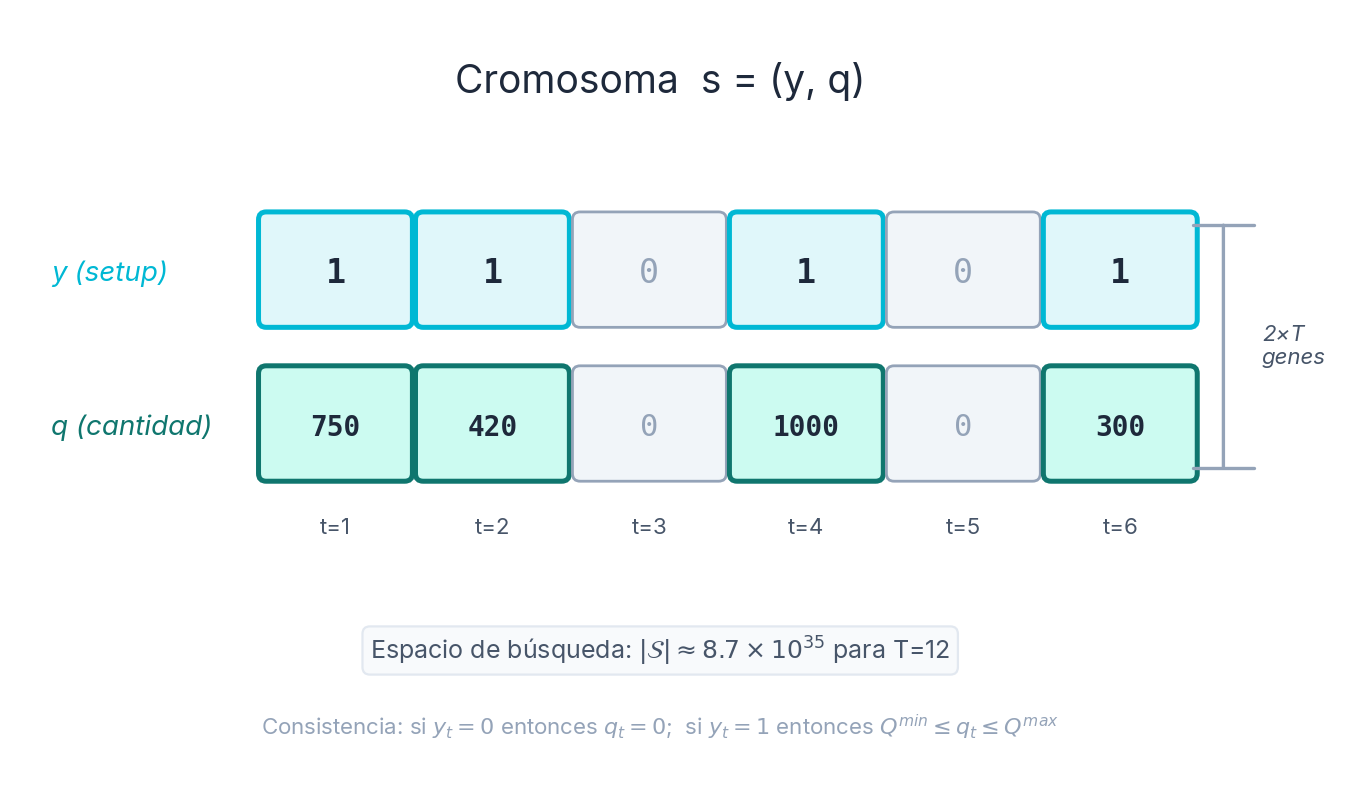
\includegraphics[width=0.85\linewidth,height=\textheight,keepaspectratio,alt={@SHORT?@Representación? visual del cromosoma@ENDSHORT?@@ Representación visual del cromosoma. Las celdas activas (y\_t = 1) se destacan con fondo cian para el vector de setup y verde para el vector de cantidad Periodos inactivos (y\_t = 0, q\_t = 0) se muestran en gris. La correspondencia posicional garantiza la consistencia: si y\_t = 0, necesariamente q\_t = 0; si y\_t = 1, entonces Q\^{}\{min\} \textbackslash leq q\_t \textbackslash leq Q\^{}\{max\}.}]{figuras/fig_chromosome_representation.png}
\caption{@\textbf{SHORT?}@\textbf{Representación?} visual del
cromosoma@\textbf{ENDSHORT?}@@ Representación visual del cromosoma. Las
celdas activas (\(y_t = 1\)) se destacan con fondo cian para el vector
de setup y verde para el vector de cantidad Periodos inactivos
(\(y_t = 0\), \(q_t = 0\)) se muestran en gris. La correspondencia
posicional garantiza la consistencia: si \(y_t = 0\), necesariamente
\(q_t = 0\); si \(y_t = 1\), entonces
\(Q^{min} \leq q_t \leq Q^{max}\).}\label{fig:fig_5b}
\end{figure}

\textbf{Tamaño del espacio de búsqueda.} El espacio de soluciones
factibles \(\mathcal{S}\) tiene cardinalidad:

\begin{equation}
|\mathcal{S}| = \sum_{k=0}^{n_t} \binom{n_t}{k} \cdot (Q^{max} - Q^{min} + 1)^k
\end{equation}

donde \(k\) es el número de periodos activos. Para la instancia Medium
(\(n_t = 12\), \(Q^{min} = 100\), \(Q^{max} = 1000\)), esto equivale a
\(|\mathcal{S}| = (1 + 901)^{12} \approx 8.7 \times 10^{35}\), un
espacio que impide la enumeración exhaustiva y justifica el uso de
metaheurísticas.

\subsubsection{6.2. Operadores de
Vecindad}\label{operadores-de-vecindad}

Los \textbf{operadores de vecindad} definen la estructura del espacio de
búsqueda al determinar qué soluciones son ``alcanzables'' desde una
solución dada en un solo movimiento. Estos operadores son utilizados
directamente por el Recocido Simulado (SA, §6.8) y por la fase de
búsqueda local del híbrido GA-SA (§6.10).

Se definen tres estructuras de vecindad, cada una diseñada para
perturbar un aspecto diferente del cromosoma:

\textbf{Definición 1 --- Vecindad de Toggle (exploración estructural).}
Dado un cromosoma \(\mathbf{s} = (\mathbf{y}, \mathbf{q})\), la vecindad
de toggle \(N_{toggle}(\mathbf{s}, k)\) genera un vecino invirtiendo
\(k\) bits seleccionados aleatoriamente del vector de setup:

\begin{equation}
N_{toggle}(\mathbf{s}, k): \quad y'_{t_i} = \neg y_{t_i}, \quad \{t_1, ..., t_k\} \subset T \text{ aleatorio}
\end{equation}

Este operador modifica la \textbf{estructura de producción} (qué
periodos producen), generando movimientos de largo alcance en el espacio
de soluciones. Por defecto, \(k = 1\).

\textbf{Definición 2 --- Vecindad de Cantidad (explotación local).} La
vecindad de cantidad \(N_{quantity}(\mathbf{s}, \delta)\) perturba el
vector de cantidades con ruido gaussiano, solo en periodos activos:

\begin{equation}
N_{quantity}(\mathbf{s}, \delta): \quad q'_t = \text{clamp}\left(q_t + \mathcal{N}(0, \delta \cdot Q^{max}),\; Q^{min},\; Q^{max}\right) \quad \forall t : y_t = 1
\end{equation}

donde \(\delta \in (0, 1)\) controla la magnitud de la perturbación.
Este operador realiza ajustes finos en las cantidades de producción sin
modificar la estructura de periodos activos, favoreciendo la
\textbf{explotación local}.

\textbf{Definición 3 --- Vecindad Mixta (balance
exploración-explotación).} El SA utiliza una selección probabilística
entre las tres opciones en cada iteración:

\begin{itemize}
\tightlist
\item
  Con probabilidad \(p_{toggle}\): aplicar \(N_{toggle}\)
\item
  Con probabilidad \(p_{quantity}\): aplicar \(N_{quantity}\)
\item
  Con probabilidad \(1 - p_{toggle} - p_{quantity}\): aplicar ambas
  secuencialmente
\end{itemize}

Este mecanismo permite al SA alternar entre movimientos exploratorios
(cambiar estructura) y explotatorios (refinar cantidades) de manera
adaptativa.

\begin{longtable}[]{@{}
  >{\raggedright\arraybackslash}p{(\linewidth - 14\tabcolsep) * \real{0.1000}}
  >{\centering\arraybackslash}p{(\linewidth - 14\tabcolsep) * \real{0.1333}}
  >{\centering\arraybackslash}p{(\linewidth - 14\tabcolsep) * \real{0.1333}}
  >{\centering\arraybackslash}p{(\linewidth - 14\tabcolsep) * \real{0.1333}}
  >{\centering\arraybackslash}p{(\linewidth - 14\tabcolsep) * \real{0.1333}}
  >{\centering\arraybackslash}p{(\linewidth - 14\tabcolsep) * \real{0.1333}}
  >{\centering\arraybackslash}p{(\linewidth - 14\tabcolsep) * \real{0.1333}}
  >{\raggedright\arraybackslash}p{(\linewidth - 14\tabcolsep) * \real{0.1000}}@{}}
\caption{Ejemplo de aplicación de operadores de vecindad sobre un
cromosoma con \(n_t = 6\) \{\#tbl:tabla\_5b\}}\tabularnewline
\toprule\noalign{}
\begin{minipage}[b]{\linewidth}\raggedright
\end{minipage} & \begin{minipage}[b]{\linewidth}\centering
\(t=1\)
\end{minipage} & \begin{minipage}[b]{\linewidth}\centering
\(t=2\)
\end{minipage} & \begin{minipage}[b]{\linewidth}\centering
\(t=3\)
\end{minipage} & \begin{minipage}[b]{\linewidth}\centering
\(t=4\)
\end{minipage} & \begin{minipage}[b]{\linewidth}\centering
\(t=5\)
\end{minipage} & \begin{minipage}[b]{\linewidth}\centering
\(t=6\)
\end{minipage} & \begin{minipage}[b]{\linewidth}\raggedright
Acción
\end{minipage} \\
\midrule\noalign{}
\endfirsthead
\toprule\noalign{}
\begin{minipage}[b]{\linewidth}\raggedright
\end{minipage} & \begin{minipage}[b]{\linewidth}\centering
\(t=1\)
\end{minipage} & \begin{minipage}[b]{\linewidth}\centering
\(t=2\)
\end{minipage} & \begin{minipage}[b]{\linewidth}\centering
\(t=3\)
\end{minipage} & \begin{minipage}[b]{\linewidth}\centering
\(t=4\)
\end{minipage} & \begin{minipage}[b]{\linewidth}\centering
\(t=5\)
\end{minipage} & \begin{minipage}[b]{\linewidth}\centering
\(t=6\)
\end{minipage} & \begin{minipage}[b]{\linewidth}\raggedright
Acción
\end{minipage} \\
\midrule\noalign{}
\endhead
\bottomrule\noalign{}
\endlastfoot
\(\mathbf{y}\) Original & 1 & 1 & 0 & 1 & 0 & 1 & --- \\
\(\mathbf{q}\) Original & 750 & 420 & 0 & 1000 & 0 & 300 & --- \\
\(\mathbf{y}'\) Toggle (\(t_1=3\)) & 1 & 1 & \textbf{1} & 1 & 0 & 1 &
Activar \(t=3\) \\
\(\mathbf{q}'\) Toggle & 750 & 420 & \textbf{537} & 1000 & 0 & 300 &
\(q'_3 \sim U[100, 1000]\) \\
\(\mathbf{q}'\) Cantidad (\(\delta=0.15\)) & \textbf{712} & \textbf{480}
& 0 & \textbf{955} & 0 & \textbf{328} & Perturbación global \\
\end{longtable}

\begin{figure}
\centering
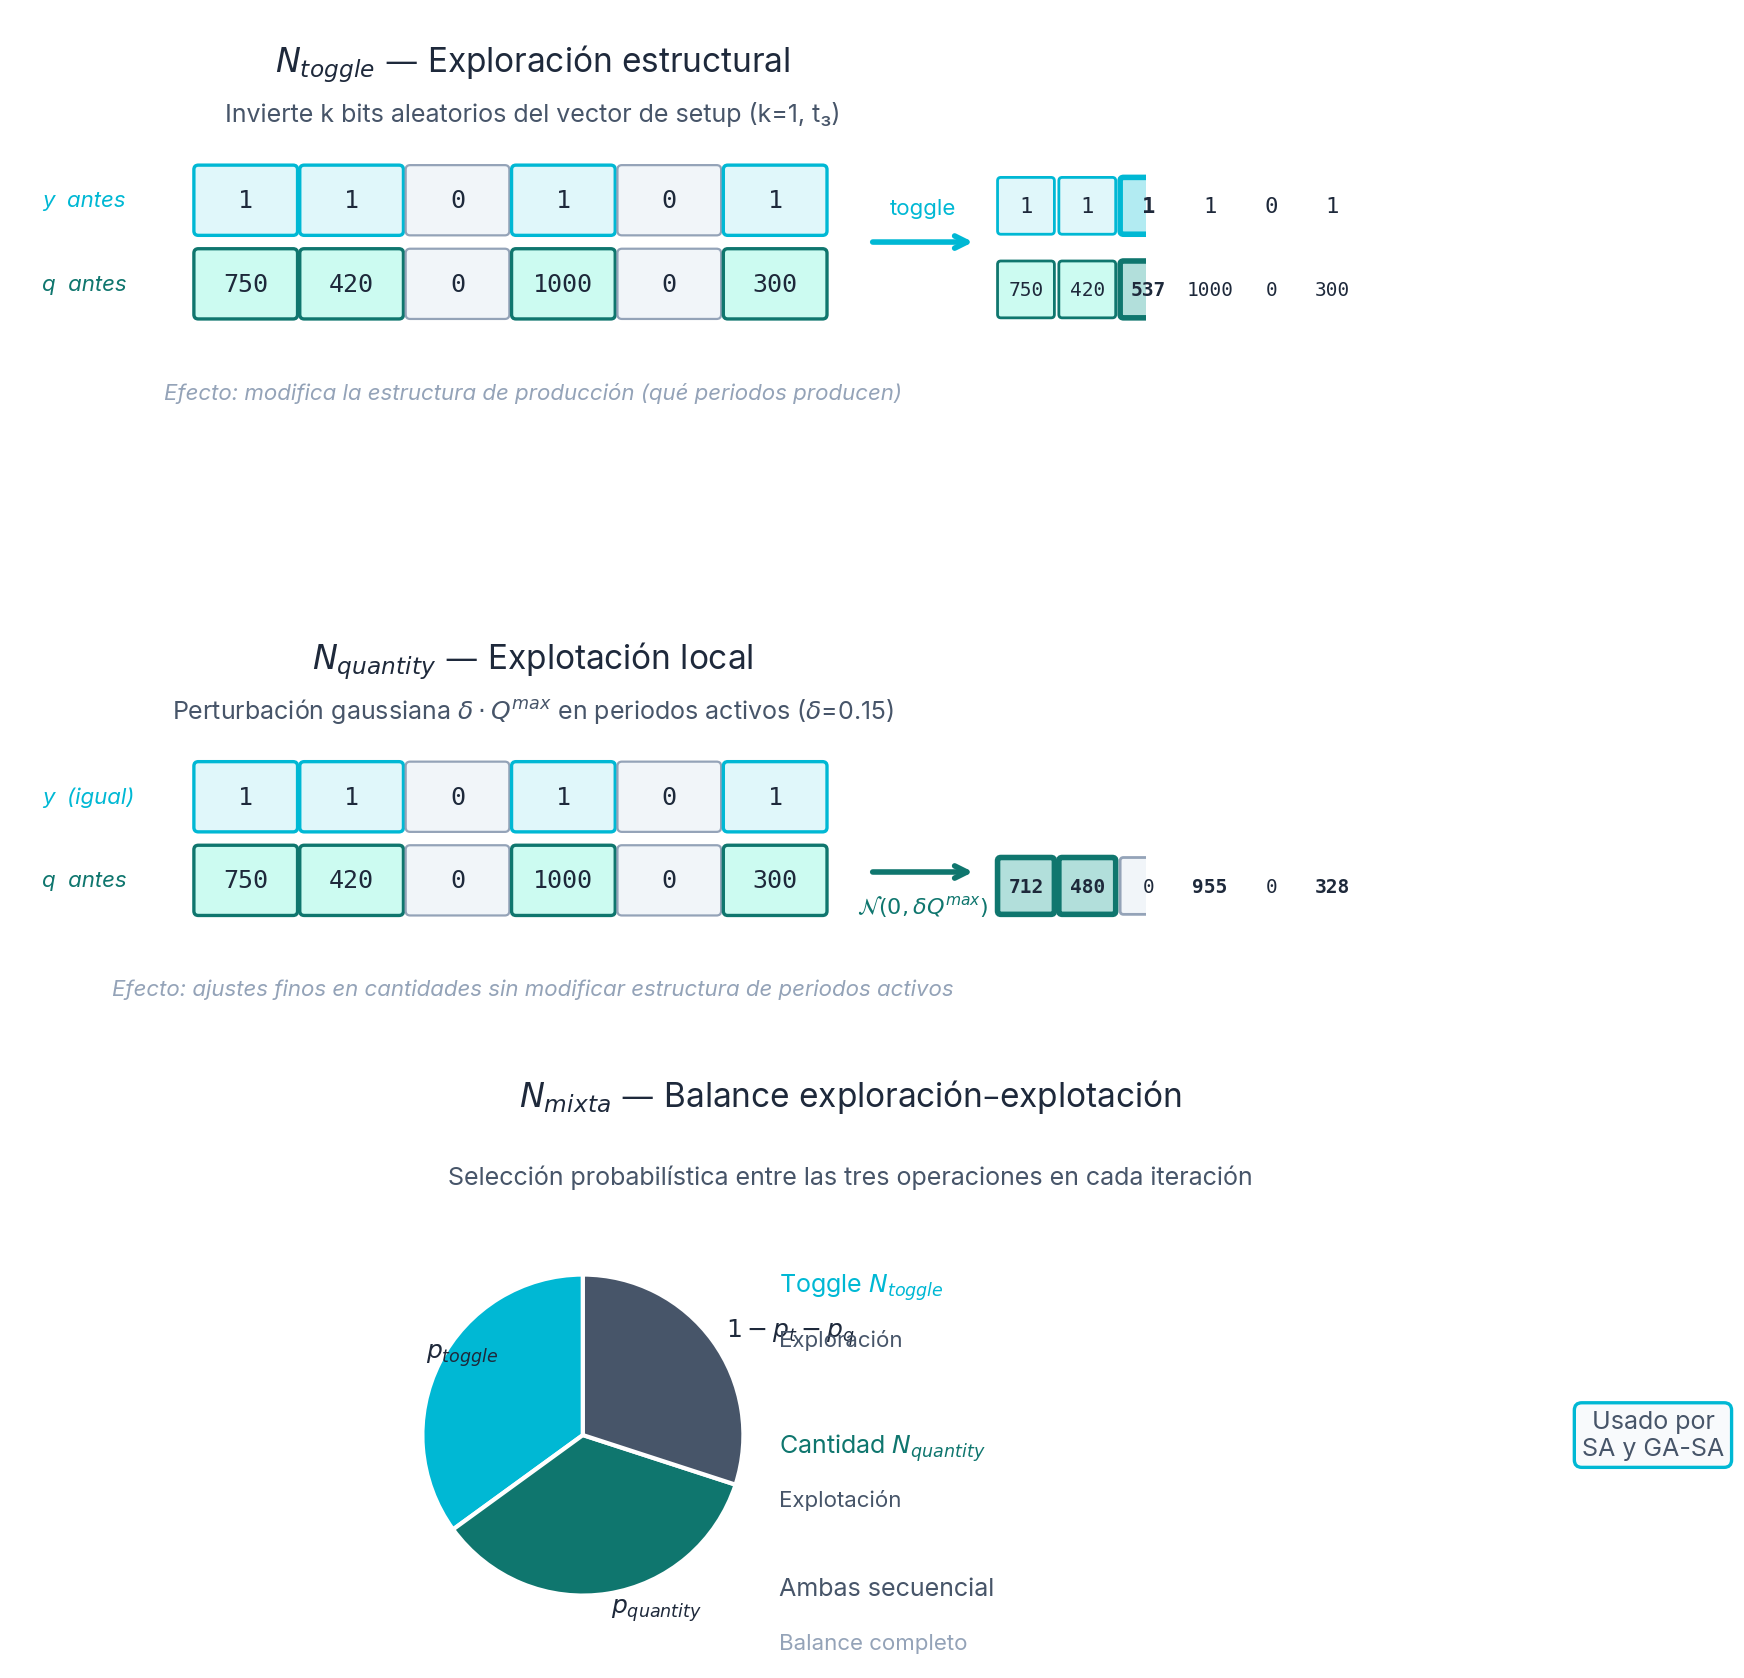
\includegraphics[width=0.9\linewidth,height=\textheight,keepaspectratio,alt={@SHORT?@Representación? visual de los tres operadores de vecindad@ENDSHORT?@@ Representación visual de los tres operadores de vecindad. El operador toggle (N\_\{toggle\}) modifica la estructura de periodos activos invirtiendo bits del vector de setup. El operador de cantidad (N\_\{quantity\}) perturba las cantidades de producción con ruido gaussiano. El operador mixto (N\_\{mixta\}) selecciona probabilísticamente entre ambos, logrando un balance entre exploración y explotación.}]{figuras/fig_neighborhood_operators.png}
\caption{@\textbf{SHORT?}@\textbf{Representación?} visual de los tres
operadores de vecindad@\textbf{ENDSHORT?}@@ Representación visual de los
tres operadores de vecindad. El operador toggle (\(N_{toggle}\))
modifica la estructura de periodos activos invirtiendo bits del vector
de setup. El operador de cantidad (\(N_{quantity}\)) perturba las
cantidades de producción con ruido gaussiano. El operador mixto
(\(N_{mixta}\)) selecciona probabilísticamente entre ambos, logrando un
balance entre exploración y explotación.}\label{fig:fig_5c}
\end{figure}

\subsubsection{6.3. Operadores Genéticos}\label{operadores-genuxe9ticos}

Los \textbf{operadores genéticos} son los mecanismos de variación
utilizados por los algoritmos basados en población (GA, §6.7 y GA-SA,
§6.10) para generar nuevas soluciones a partir de las existentes.

\paragraph{6.3.1. Cruce de Dos Puntos}\label{cruce-de-dos-puntos}

El cruce de dos puntos genera dos hijos intercambiando un segmento
central entre dos padres. Se seleccionan aleatoriamente dos puntos de
corte \(p_1 < p_2\) en el rango \([1, n_t-1]\), y se intercambian
simultáneamente los segmentos correspondientes de \(\mathbf{y}\) y
\(\mathbf{q}\):

\begin{equation}
\mathbf{y}^{hijo1} = (y^{P1}_1, ..., y^{P1}_{p_1}, \underbrace{y^{P2}_{p_1+1}, ..., y^{P2}_{p_2}}_{\text{segmento de } P2}, y^{P1}_{p_2+1}, ..., y^{P1}_{n_t})
\end{equation}

El mismo patrón de intercambio se aplica al vector \(\mathbf{q}\). Tras
el cruce, se aplica el mecanismo de reparación (§6.4) para garantizar
factibilidad.

\begin{longtable}[]{@{}lcccccc@{}}
\caption{Ejemplo de cruce de dos puntos con \(p_1 = 2\), \(p_2 = 4\)
\{\#tbl:tabla\_5c\}}\tabularnewline
\toprule\noalign{}
& \(t=1\) & \(t=2\) & \(t=3\) & \(t=4\) & \(t=5\) & \(t=6\) \\
\midrule\noalign{}
\endfirsthead
\toprule\noalign{}
& \(t=1\) & \(t=2\) & \(t=3\) & \(t=4\) & \(t=5\) & \(t=6\) \\
\midrule\noalign{}
\endhead
\bottomrule\noalign{}
\endlastfoot
\textbf{Padre 1} \(\mathbf{y}\) & 1 & 1 & 0 & 1 & 0 & 1 \\
\textbf{Padre 1} \(\mathbf{q}\) & 750 & 420 & 0 & 1000 & 0 & 300 \\
\textbf{Padre 2} \(\mathbf{y}\) & 0 & 1 & 1 & 0 & 1 & 1 \\
\textbf{Padre 2} \(\mathbf{q}\) & 0 & 600 & 350 & 0 & 800 & 500 \\
\textbf{Hijo 1} \(\mathbf{y}\) & 1 & 1 & \textbf{1} & \textbf{0} & 0 &
1 \\
\textbf{Hijo 1} \(\mathbf{q}\) & 750 & 420 & \textbf{350} & \textbf{0} &
0 & 300 \\
\textbf{Hijo 2} \(\mathbf{y}\) & 0 & 1 & \textbf{0} & \textbf{1} & 1 &
1 \\
\textbf{Hijo 2} \(\mathbf{q}\) & 0 & 600 & \textbf{0} & \textbf{1000} &
800 & 500 \\
\end{longtable}

\paragraph{6.3.2. Mutación Mixta}\label{mutaciuxf3n-mixta}

La mutación opera gen por gen sobre el cromosoma, aplicando dos tipos de
perturbación de manera independiente:

\begin{enumerate}
\def\labelenumi{\arabic{enumi}.}
\item
  \textbf{Toggle de setup:} Para cada gen \(y_t\), se invierte con
  probabilidad \(p_{toggle}\):
  \[y'_t = \begin{cases} \neg y_t & \text{con probabilidad } p_{toggle} \\ y_t & \text{con probabilidad } 1 - p_{toggle} \end{cases}\]
\item
  \textbf{Perturbación de cantidad:} Para cada gen \(q_t\) con
  \(y'_t = 1\), se perturba con probabilidad \(p_{quantity}\):
  \[q'_t = \text{clamp}(q_t + \mathcal{N}(0, \delta \cdot Q^{max}), Q^{min}, Q^{max})\]
\end{enumerate}

Los valores típicos calibrados son \(p_{toggle} \approx 0.05\)--\(0.10\)
y \(\delta \approx 0.07\)--\(0.15\) (Tabla 5d, §6.11).

\subsubsection{6.4. Mecanismo de
Reparación}\label{mecanismo-de-reparaciuxf3n}

Tras la aplicación de cualquier operador (vecindad, cruce o mutación),
el cromosoma resultante puede violar las restricciones de consistencia
entre \(\mathbf{y}\) y \(\mathbf{q}\). El \textbf{mecanismo de
reparación} (\texttt{repair\_lot\_sizing}) aplica las siguientes reglas
en orden, garantizando factibilidad:

\begin{enumerate}
\def\labelenumi{\arabic{enumi}.}
\tightlist
\item
  \textbf{Activación implícita:} Si \(q_t > 0\) y \(y_t = 0\), se activa
  el setup: \(y_t \leftarrow 1\).
\item
  \textbf{Desactivación coherente:} Si \(y_t = 0\), se fuerza:
  \(q_t \leftarrow 0\).
\item
  \textbf{Acotamiento de capacidad:} Si \(y_t = 1\), se ajusta:
  \(q_t \leftarrow \text{clamp}(q_t, Q^{min}, Q^{max})\).
\end{enumerate}

Este mecanismo garantiza que \textbf{todo cromosoma generado durante la
búsqueda es factible} respecto a las restricciones de primera etapa
(Restricciones 3 y 4 del modelo, §5.3), eliminando la necesidad de
penalizaciones por infactibilidad. La factibilidad de segunda etapa
(balance de materiales, perecibilidad) se garantiza por construcción del
decodificador greedy (§6.6).

\subsubsection{6.5. Balance Exploración--Explotación del Espacio de
Soluciones}\label{balance-exploraciuxf3nexplotaciuxf3n-del-espacio-de-soluciones}

La eficacia de una metaheurística depende crucialmente del
\textbf{balance entre exploración} (diversificación: visitar regiones
nuevas del espacio de búsqueda) y \textbf{explotación} (intensificación:
refinar soluciones prometedoras en la vecindad de un óptimo local). La
Tabla 5d resume cómo cada mecanismo y algoritmo contribuye a este
balance.

\begin{longtable}[]{@{}
  >{\raggedright\arraybackslash}p{(\linewidth - 6\tabcolsep) * \real{0.1746}}
  >{\centering\arraybackslash}p{(\linewidth - 6\tabcolsep) * \real{0.0952}}
  >{\centering\arraybackslash}p{(\linewidth - 6\tabcolsep) * \real{0.1905}}
  >{\raggedright\arraybackslash}p{(\linewidth - 6\tabcolsep) * \real{0.5397}}@{}}
\caption{@\textbf{SHORT?}@\textbf{Clasificación?} de mecanismos según su
contribución a exploración vs@\textbf{ENDSHORT?}@@ Clasificación de
mecanismos según su contribución a exploración vs.~explotación
\{\#tbl:tabla\_5d\}}\tabularnewline
\toprule\noalign{}
\begin{minipage}[b]{\linewidth}\raggedright
Mecanismo
\end{minipage} & \begin{minipage}[b]{\linewidth}\centering
Tipo
\end{minipage} & \begin{minipage}[b]{\linewidth}\centering
Algoritmos
\end{minipage} & \begin{minipage}[b]{\linewidth}\raggedright
Efecto en el espacio de búsqueda
\end{minipage} \\
\midrule\noalign{}
\endfirsthead
\toprule\noalign{}
\begin{minipage}[b]{\linewidth}\raggedright
Mecanismo
\end{minipage} & \begin{minipage}[b]{\linewidth}\centering
Tipo
\end{minipage} & \begin{minipage}[b]{\linewidth}\centering
Algoritmos
\end{minipage} & \begin{minipage}[b]{\linewidth}\raggedright
Efecto en el espacio de búsqueda
\end{minipage} \\
\midrule\noalign{}
\endhead
\bottomrule\noalign{}
\endlastfoot
Toggle de setup (\(N_{toggle}\)) & Exploración & SA, GA-SA & Modifica
estructura de periodos activos; saltos largos \\
Perturbación de cantidad (\(N_{quantity}\)) & Explotación & SA, GA-SA &
Ajusta finamente cantidades; movimientos cortos \\
Cruce de dos puntos & Exploración & GA, GA-SA & Recombina segmentos de
soluciones diversas \\
Mutación mixta (toggle + gaussiana) & Exploración & GA, GA-SA &
Introduce variabilidad aleatoria gen por gen \\
Selección por torneo & Explotación & GA, GA-SA & Presiona hacia
soluciones de alta calidad \\
Elitismo (top-\(e\)) & Explotación & GA, GA-SA & Preserva las mejores
soluciones entre generaciones \\
Criterio de Metropolis & Balance & SA, GA-SA & Acepta peores soluciones
con \(P = e^{\Delta/T}\) \\
Enfriamiento geométrico & Exploración→Explotación & SA & Transición
gradual de exploración a explotación \\
Reheating adaptativo & Exploración & SA & Reactiva exploración ante
estancamiento \\
Mutación diferencial (\(F \cdot (x_{r1} - x_{r2})\)) & Exploración
dirigida & DE & Utiliza diferencias poblacionales como dirección de
búsqueda \\
Selección greedy (trial vs.~target) & Explotación & DE & Solo acepta
mejoras; presión selectiva fuerte \\
Búsqueda local SA periódica & Explotación & GA-SA & Refina los mejores
individuos de la población \\
\end{longtable}

La \textbf{combinación de estos mecanismos} es lo que confiere a cada
algoritmo su perfil de búsqueda característico:

\begin{itemize}
\tightlist
\item
  \textbf{GA (§6.7):} Exploración predominante mediante población
  diversa y operadores genéticos (cruce + mutación), con explotación
  limitada por elitismo y presión de torneo.
\item
  \textbf{SA (§6.8):} Trayectoria individual que transita de exploración
  (alta temperatura) a explotación (baja temperatura), con reheating
  para escapar de óptimos locales.
\item
  \textbf{DE (§6.9):} Exploración dirigida mediante vectores de
  diferencia, combinada con explotación fuerte por selección greedy (el
  trial solo sobrevive si supera al target).
\item
  \textbf{GA-SA (§6.10):} Balance óptimo --- la exploración global del
  GA se complementa con la explotación local del SA aplicado
  periódicamente a los mejores individuos (Figura 19 confirma que GA-SA
  mantiene mayor diversidad que GA puro).
\end{itemize}

\begin{figure}
\centering
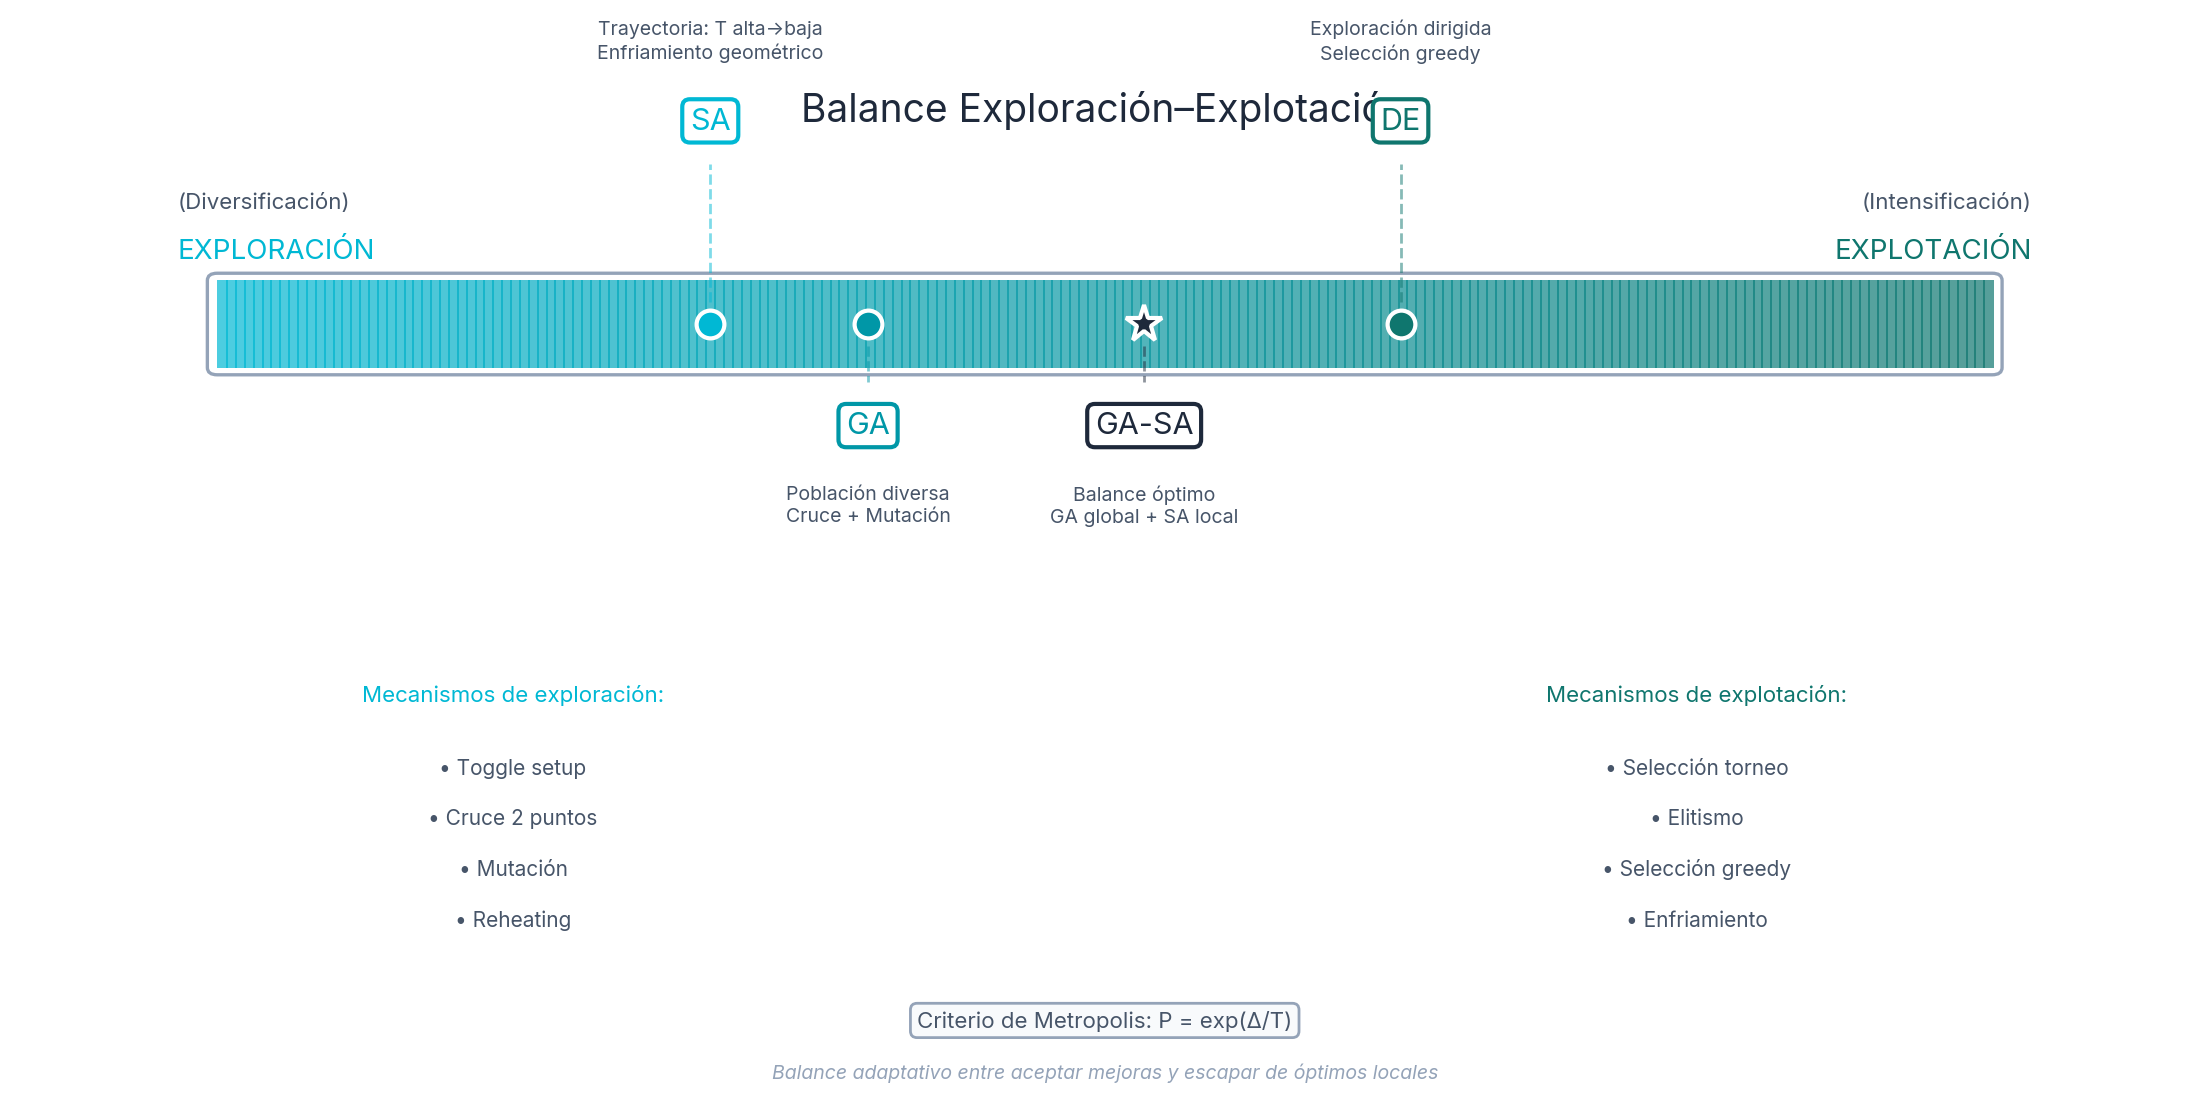
\includegraphics[width=0.9\linewidth,height=\textheight,keepaspectratio,alt={@SHORT?@Posicionamiento? de los cuatro algoritmos en el espectro exploración--explotación@ENDSHORT?@@ Posicionamiento de los cuatro algoritmos en el espectro exploración--explotación. SA se ubica hacia la exploración (alta temperatura inicial) con transición gradual a explotación (enfriamiento). GA prioriza diversificación mediante población y operadores genéticos. DE combina exploración dirigida con selección greedy. GA-SA logra el balance óptimo al complementar la exploración global del GA con la explotación local del SA.}]{figuras/fig_exploration_exploitation.png}
\caption{@\textbf{SHORT?}@\textbf{Posicionamiento?} de los cuatro
algoritmos en el espectro exploración--explotación@\textbf{ENDSHORT?}@@
Posicionamiento de los cuatro algoritmos en el espectro
exploración--explotación. SA se ubica hacia la exploración (alta
temperatura inicial) con transición gradual a explotación
(enfriamiento). GA prioriza diversificación mediante población y
operadores genéticos. DE combina exploración dirigida con selección
greedy. GA-SA logra el balance óptimo al complementar la exploración
global del GA con la explotación local del SA.}\label{fig:fig_5d}
\end{figure}

\subsubsection{6.6. Decodificador Greedy}\label{decodificador-greedy}

Dado un par \((\mathbf{y}, \mathbf{q})\), el decodificador calcula las
variables de segunda etapa \((\mathbf{v}, \mathbf{I}, \mathbf{u})\) para
cada escenario \(\omega\) mediante una asignación greedy:

\begin{enumerate}
\def\labelenumi{\arabic{enumi}.}
\tightlist
\item
  \textbf{Producción por forma de corte:} Se asigna la masa anatómica
  disponible (\(\alpha_p \cdot W \cdot q_t\)) a las formas de corte por
  orden descendente de precio, respetando la disponibilidad por pieza
  anatómica.
\item
  \textbf{Ventas FIFO:} Para cada forma de corte en cada escenario, las
  ventas se asignan consumiendo inventario en orden FIFO (el más antiguo
  se vende primero), respetando la restricción de demanda.
\item
  \textbf{Inventario residual:} El inventario al final de cada periodo
  es la diferencia entre disponibilidad y ventas.
\end{enumerate}

Este decodificador es determinista: dado \((\mathbf{y}, \mathbf{q})\) y
una instancia, siempre produce el mismo resultado.

\subsubsection{6.7. Algoritmo Genético
(GA)}\label{algoritmo-genuxe9tico-ga}

El GA opera sobre una población de \(N\) individuos, cada uno codificado
como \((\mathbf{y}, \mathbf{q})\). Los operadores están adaptados a
variables mixtas (binarias + enteras):

\begin{itemize}
\tightlist
\item
  \textbf{Selección:} Torneo de tamaño \(k\) --- selecciona el mejor
  individuo entre \(k\) candidatos aleatorios.
\item
  \textbf{Cruce:} Cruce de dos puntos aplicado independientemente a
  \(\mathbf{y}\) y \(\mathbf{q}\), respetando los límites
  \([Q^{min}, Q^{max}]\).
\item
  \textbf{Mutación:} Bit-flip para \(\mathbf{y}\) (con probabilidad
  \(p_{toggle}\)) y perturbación gaussiana acotada para \(\mathbf{q}\)
  (\(\delta = 15\%\) del rango).
\item
  \textbf{Elitismo:} Los \(e\) mejores individuos pasan directamente a
  la siguiente generación.
\item
  \textbf{Criterio de parada:} Estancamiento (sin mejora durante \(s\)
  generaciones consecutivas).
\end{itemize}

\protect\phantomsection\label{fig:fig_6}
Diagrama de flujo del Algoritmo Genético (GA) con operadores de cruce de
dos puntos, mutación mixta y elitismo.

\subsubsection{6.8. Recocido Simulado (SA)}\label{recocido-simulado-sa}

El SA utiliza un esquema de enfriamiento geométrico con \emph{reheating}
adaptativo:

\begin{itemize}
\tightlist
\item
  \textbf{Temperatura inicial:} Auto-estimada mediante 20 pares de
  soluciones aleatorias, calibrada para aceptar \textasciitilde80\% de
  soluciones inicialmente (\(T_0 = -\bar{\Delta} / \ln(0.8)\)).
\item
  \textbf{Enfriamiento geométrico:} \(T_{k+1} = \alpha \cdot T_k\) con
  \(\alpha = 0.78\).
\item
  \textbf{Vecindarios mixtos:} Con probabilidad \(p_{toggle}\) alterna
  un setup, con \(p_{quantity}\) perturba una cantidad, y con
  \(1 - p_{toggle} - p_{quantity}\) aplica ambas perturbaciones.
\item
  \textbf{Criterio de Metropolis:} Acepta una solución peor \(s'\) con
  probabilidad \(\exp(\Delta / T)\) donde \(\Delta = f(s') - f(s)\).
\item
  \textbf{Reheating:} Cuando se estanca por \(r\) iteraciones sin
  mejora, la temperatura se multiplica por un factor \(> 1\) para
  reactivar la exploración.
\end{itemize}

\protect\phantomsection\label{fig:fig_7}
Diagrama de flujo del Recocido Simulado (SA) con enfriamiento
geométrico, vecindarios mixtos y reheating adaptativo.

\subsubsection{6.9. Evolución Diferencial
(DE)}\label{evoluciuxf3n-diferencial-de}

El DE opera sobre una población de vectores continuos en
\([0, 1]^{2n_t}\) que se discretizan para evaluar:

\begin{itemize}
\tightlist
\item
  \textbf{Codificación continua:} Cada individuo es un vector
  \(\mathbf{x} \in [0,1]^{2n_t}\) donde las primeras \(n_t\) componentes
  codifican \(\mathbf{y}\) (umbral 0.5) y las siguientes \(n_t\)
  codifican \(\mathbf{q}\) (normalizado en \([Q^{min}, Q^{max}]\)).
\item
  \textbf{Mutación DE:} Vector mutante
  \(\mathbf{v} = \mathbf{x}_{best} + F \cdot (\mathbf{x}_{r1} - \mathbf{x}_{r2})\)
  (estrategia best/1/bin).
\item
  \textbf{Cruce binomial:} Cada componente del vector trial se toma del
  mutante con probabilidad \(CR\) o del target con \(1-CR\).
\item
  \textbf{Selección greedy:} El trial reemplaza al target solo si tiene
  mejor fitness.
\end{itemize}

\protect\phantomsection\label{fig:fig_8}
Diagrama de flujo de la Evolución Diferencial (DE) con estrategia
DE/best/1/bin y codificación continua discretizada.

\subsubsection{6.10. Algoritmo Híbrido
GA-SA}\label{algoritmo-huxedbrido-ga-sa}

El GA-SA es un \textbf{algoritmo memético} que combina la exploración
global del GA con la explotación local del SA {[}15{]}:

\begin{itemize}
\tightlist
\item
  \textbf{Fase GA (global):} Idéntica al GA estándar (selección, cruce,
  mutación, elitismo).
\item
  \textbf{Fase SA (local):} Cada \(f_{LS}\) generaciones, se aplica un
  SA corto (pocas iteraciones, temperatura baja) a los \(k\) mejores
  individuos de la población, mejorando localmente las mejores
  soluciones encontradas.
\end{itemize}

\protect\phantomsection\label{fig:fig_9}
@\textbf{SHORT?}@\textbf{Diagrama?} de flujo del algoritmo híbrido
GA-SA@\textbf{ENDSHORT?}@@ Diagrama de flujo del algoritmo híbrido
GA-SA. La búsqueda local SA se activa periódicamente sobre los mejores
individuos de la población.

\subsubsection{6.11. Calibración de Hiperparámetros
(Optuna/TPE)}\label{calibraciuxf3n-de-hiperparuxe1metros-optunatpe}

Los hiperparámetros de cada metaheurística se calibraron mediante
\textbf{Optuna} con el sampler \textbf{Tree-structured Parzen Estimator
(TPE)}, evaluando sobre \textbf{5 instancias de calibración}
(\texttt{small\_seed100}, \texttt{small\_seed101},
\texttt{small\_seed102}, \texttt{medium\_seed200},
\texttt{medium\_seed201}). Se ejecutaron \textbf{30 trials por
algoritmo} (timeout de 900 s por trial), con objetivo de maximizar \(Z\)
promedio.

\begin{longtable}[]{@{}lcccc@{}}
\caption{Hiperparámetros calibrados por algoritmo (resultado de
Optuna/TPE) \{\#tbl:tabla\_5e\}}\tabularnewline
\toprule\noalign{}
Parámetro & GA & SA & DE & GA-SA \\
\midrule\noalign{}
\endfirsthead
\toprule\noalign{}
Parámetro & GA & SA & DE & GA-SA \\
\midrule\noalign{}
\endhead
\bottomrule\noalign{}
\endlastfoot
\texttt{pop\_size} & 80 & --- & 51 & 39 \\
\texttt{n\_generations} / \texttt{max} & 200 & --- & 200 & 200 \\
\texttt{crossover\_rate} & 0.744 & --- & --- & 0.859 \\
\texttt{mutation\_rate} & 0.089 & --- & --- & 0.051 \\
\texttt{elitism\_count} & 3 & --- & --- & 1 \\
\texttt{selection\_size} & 3 & --- & --- & 3 \\
\texttt{T\_initial} & --- & 203,952 & --- & --- \\
\texttt{T\_final} & --- & 586 & --- & --- \\
\texttt{cooling\_rate} & --- & 0.782 & --- & --- \\
\texttt{delta} & --- & 0.066 & --- & --- \\
\texttt{max\_iterations} & --- & 27 & --- & --- \\
\texttt{p\_toggle} & --- & 0.494 & --- & --- \\
\texttt{p\_quantity} & --- & 0.283 & --- & --- \\
\texttt{reheat\_factor} & --- & 1.287 & --- & --- \\
\texttt{F} (escala) & --- & --- & 0.317 & --- \\
\texttt{CR} (cruce) & --- & --- & 0.511 & --- \\
\texttt{strategy} & --- & --- & best/1/bin & --- \\
\texttt{local\_search\_freq} & --- & --- & --- & 9 \\
\texttt{local\_search\_top\_k} & --- & --- & --- & 10 \\
\texttt{local\_search\_iters} & --- & --- & --- & 26 \\
\texttt{local\_search\_T} & --- & --- & --- & 3,227 \\
\texttt{local\_search\_cooling} & --- & --- & --- & 0.713 \\
\texttt{stagnation\_limit} & 50 & 54 & 50 & 50 \\
\end{longtable}

\begin{figure}
\centering
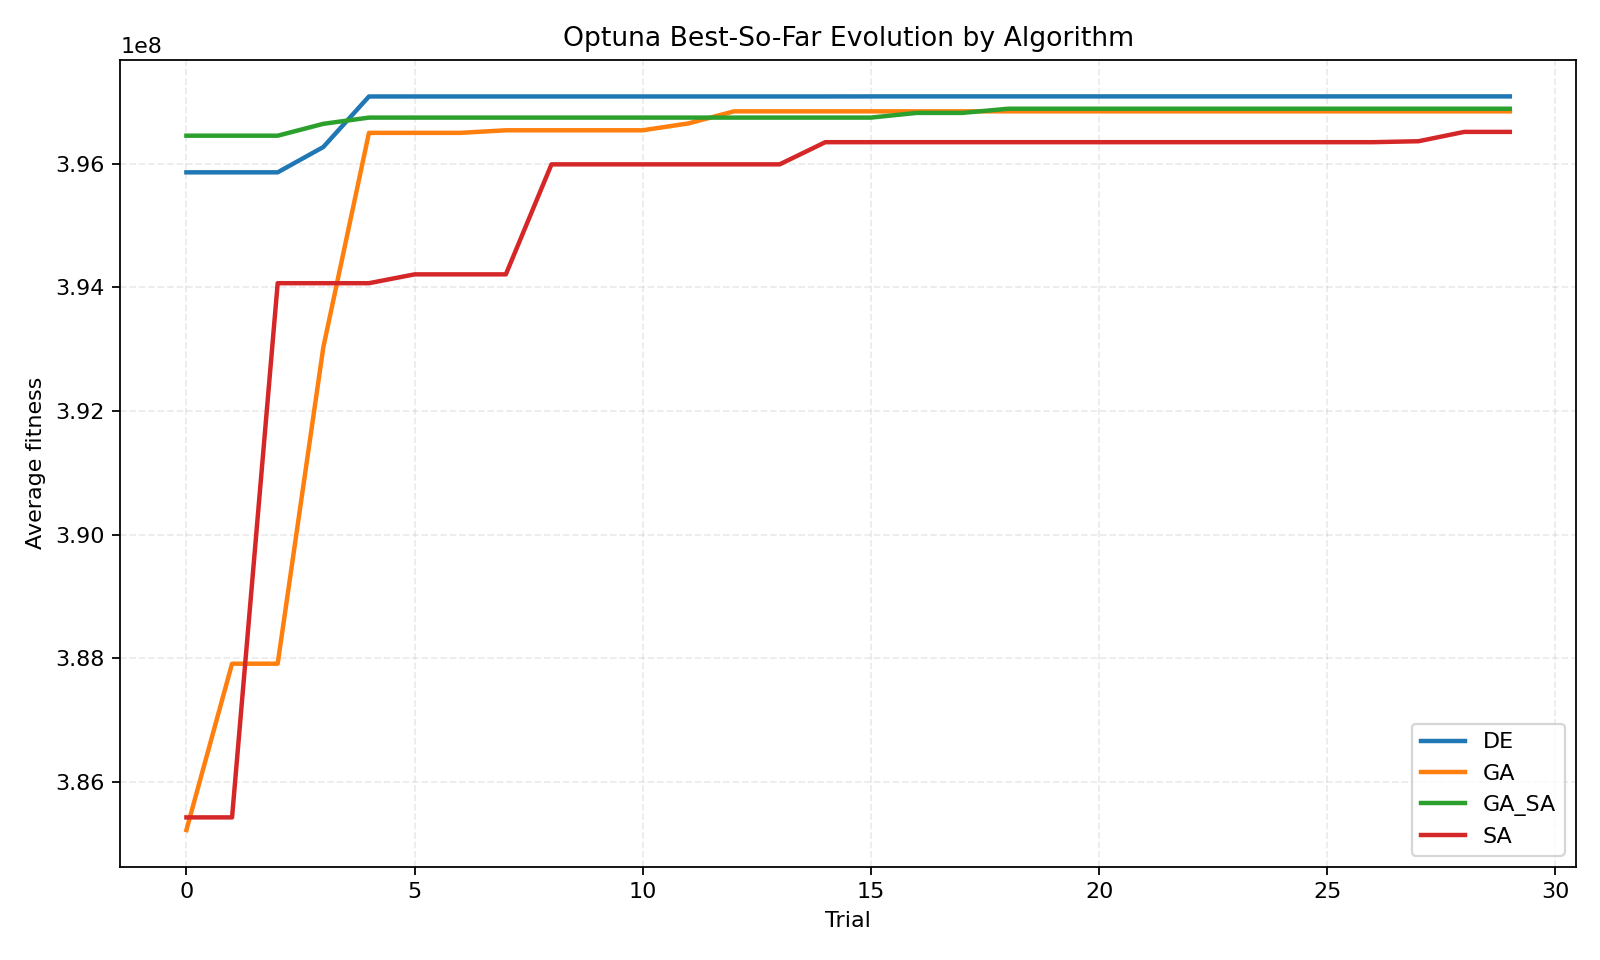
\includegraphics[width=0.8\linewidth,height=\textheight,keepaspectratio,alt={@SHORT?@Evolución? del mejor fitness durante la calibración con Optuna/TPE para cada algoritmo@ENDSHORT?@@ Evolución del mejor fitness durante la calibración con Optuna/TPE para cada algoritmo. GA-SA alcanza la convergencia más rápida, seguida por DE, GA y SA.}]{figuras/tuning_evolution_comparison.png}
\caption{@\textbf{SHORT?}@\textbf{Evolución?} del mejor fitness durante
la calibración con Optuna/TPE para cada algoritmo@\textbf{ENDSHORT?}@@
Evolución del mejor fitness durante la calibración con Optuna/TPE para
cada algoritmo. GA-SA alcanza la convergencia más rápida, seguida por
DE, GA y SA.}\label{fig:fig_10}
\end{figure}

\begin{center}\rule{0.5\linewidth}{0.5pt}\end{center}

\subsection{7. Resultados
Computacionales}\label{resultados-computacionales}

\subsubsection{7.1. Diseño Experimental}\label{diseuxf1o-experimental}

El diseño experimental sigue un esquema factorial completo con los
siguientes factores:

\begin{itemize}
\tightlist
\item
  \textbf{Factor A --- Algoritmo:} \{GA, SA, DE, GA-SA, CBC-exacto,
  Baseline\} (6 niveles)
\item
  \textbf{Factor B --- Tamaño de instancia:} \{Small, Medium, Large\} (3
  niveles)
\item
  \textbf{Instancias por tamaño:} 3 (seeds 42, 123, 456)
\item
  \textbf{Réplicas por combinación:} 30 seeds para algoritmos
  estocásticos, 1 para deterministas (CBC, Baseline)
\end{itemize}

\textbf{Total:} 4 algoritmos × 9 instancias × 30 seeds + 2 deterministas
× 9 instancias = \textbf{1,098 ejecuciones}

Cada ejecución tiene un límite de tiempo de 300 segundos. Los
experimentos se ejecutaron en Python 3.11, con checkpoints cada 50
ejecuciones para tolerancia a fallos.

\subsubsection{7.2. Perfiles de
Instancias}\label{perfiles-de-instancias}

\begin{longtable}[]{@{}
  >{\raggedright\arraybackslash}p{(\linewidth - 14\tabcolsep) * \real{0.1053}}
  >{\centering\arraybackslash}p{(\linewidth - 14\tabcolsep) * \real{0.0921}}
  >{\centering\arraybackslash}p{(\linewidth - 14\tabcolsep) * \real{0.0921}}
  >{\centering\arraybackslash}p{(\linewidth - 14\tabcolsep) * \real{0.1579}}
  >{\centering\arraybackslash}p{(\linewidth - 14\tabcolsep) * \real{0.1447}}
  >{\centering\arraybackslash}p{(\linewidth - 14\tabcolsep) * \real{0.1447}}
  >{\centering\arraybackslash}p{(\linewidth - 14\tabcolsep) * \real{0.0921}}
  >{\raggedright\arraybackslash}p{(\linewidth - 14\tabcolsep) * \real{0.1711}}@{}}
\caption{Perfiles de instancias de prueba
\{\#tbl:tabla\_6\}}\tabularnewline
\toprule\noalign{}
\begin{minipage}[b]{\linewidth}\raggedright
Perfil
\end{minipage} & \begin{minipage}[b]{\linewidth}\centering
\(n_p\)
\end{minipage} & \begin{minipage}[b]{\linewidth}\centering
\(n_t\)
\end{minipage} & \begin{minipage}[b]{\linewidth}\centering
\(n_\omega\)
\end{minipage} & \begin{minipage}[b]{\linewidth}\centering
\(Q^{min}\)
\end{minipage} & \begin{minipage}[b]{\linewidth}\centering
\(Q^{max}\)
\end{minipage} & \begin{minipage}[b]{\linewidth}\centering
Seeds
\end{minipage} & \begin{minipage}[b]{\linewidth}\raggedright
Descripción
\end{minipage} \\
\midrule\noalign{}
\endfirsthead
\toprule\noalign{}
\begin{minipage}[b]{\linewidth}\raggedright
Perfil
\end{minipage} & \begin{minipage}[b]{\linewidth}\centering
\(n_p\)
\end{minipage} & \begin{minipage}[b]{\linewidth}\centering
\(n_t\)
\end{minipage} & \begin{minipage}[b]{\linewidth}\centering
\(n_\omega\)
\end{minipage} & \begin{minipage}[b]{\linewidth}\centering
\(Q^{min}\)
\end{minipage} & \begin{minipage}[b]{\linewidth}\centering
\(Q^{max}\)
\end{minipage} & \begin{minipage}[b]{\linewidth}\centering
Seeds
\end{minipage} & \begin{minipage}[b]{\linewidth}\raggedright
Descripción
\end{minipage} \\
\midrule\noalign{}
\endhead
\bottomrule\noalign{}
\endlastfoot
Small & 5 & 6 & 10 & 100 & 1,000 & 42, 123, 456 & Validación contra CBC
óptimo \\
Medium & 8 & 12 & 50 & 100 & 1,000 & 42, 123, 456 & Escala intermedia \\
Large & 8 & 30 & 100 & 100 & 1,000 & 42, 123, 456 & Escala industrial \\
\end{longtable}

Las instancias fueron generadas con datos calibrados de la industria
avícola colombiana: proporciones anatómicas basadas en literatura,
precios de mercado FENAVI, y demanda con distribución log-normal
estacional.

\subsubsection{7.3. Resultados
Principales}\label{resultados-principales}

\begin{longtable}[]{@{}lcccc@{}}
\caption{Resultados principales por algoritmo (promedio sobre 270
ejecuciones c/u) \{\#tbl:tabla\_7\}}\tabularnewline
\toprule\noalign{}
Algoritmo & \(\bar{Z}\) (COP) & Std \(Z\) & Rank & N \\
\midrule\noalign{}
\endfirsthead
\toprule\noalign{}
Algoritmo & \(\bar{Z}\) (COP) & Std \(Z\) & Rank & N \\
\midrule\noalign{}
\endhead
\bottomrule\noalign{}
\endlastfoot
\textbf{GA-SA} & \textbf{916,865,520} & 512,578,412 & \textbf{1} &
270 \\
DE & 916,484,283 & 512,072,980 & 2 & 270 \\
GA & 908,817,120 & 501,216,075 & 3 & 270 \\
SA & 883,217,511 & 522,140,338 & 4 & 270 \\
\end{longtable}

El híbrido \textbf{GA-SA obtiene el mejor rendimiento promedio}, seguido
por DE, GA y SA. La lectura estadística depende del nivel de agregación:
en vista por corridas (ANOVA) no se observa diferencia global
(\(F = 0.259\), \(p = 0.855\)), pero al bloquear por instancia sí
aparece diferencia global (Friedman \(\chi^2 = 16.07\), \(p = 0.0011\)).
Las comparaciones pareadas con corrección Holm muestran diferencia
consistente entre SA y \{DE, GA-SA\}, mientras que \textbf{GA-SA y DE
permanecen prácticamente empatados en magnitud de efecto} (diferencia
media relativa (\approx 0.024\%)).

\begin{figure}
\centering
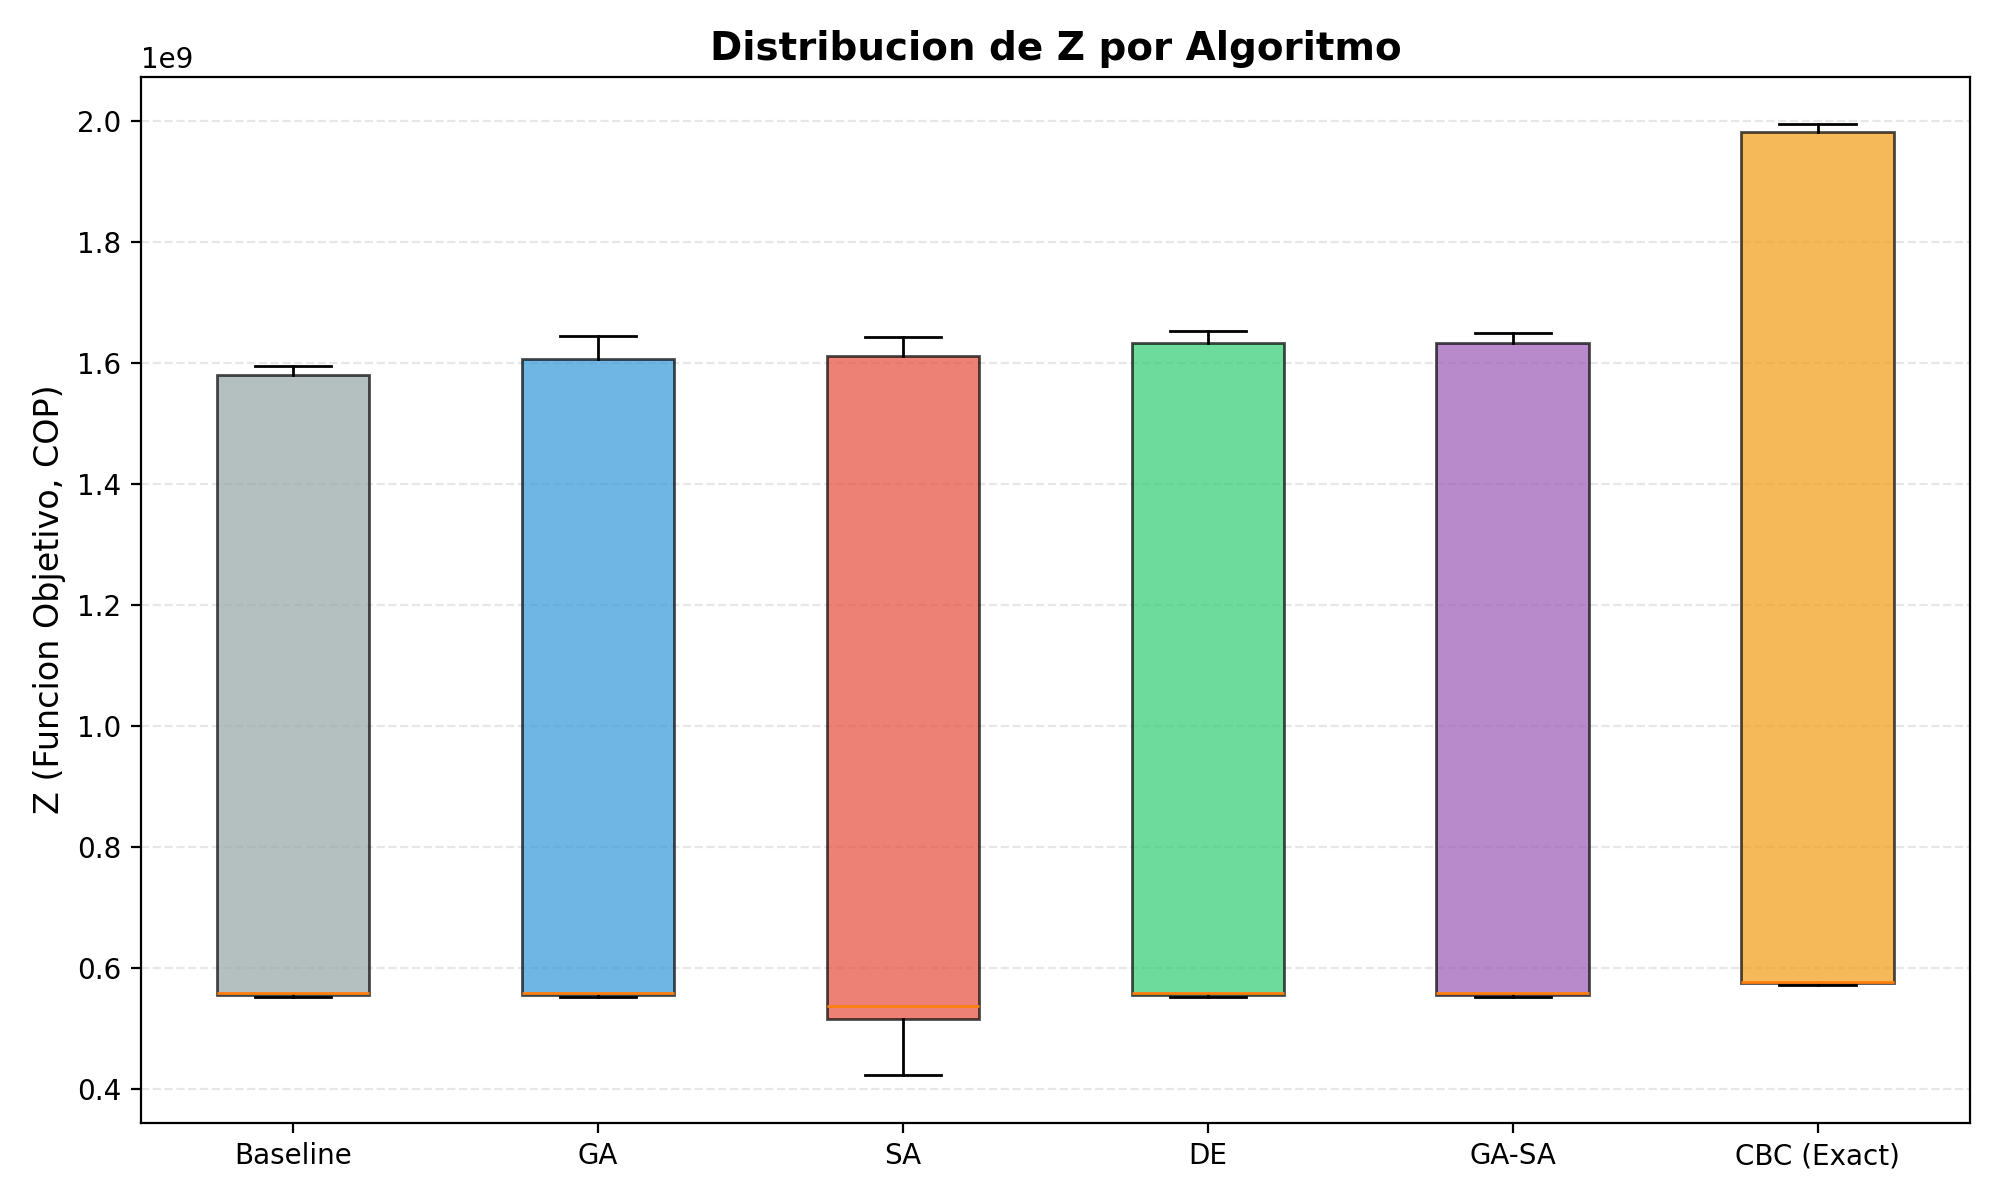
\includegraphics[width=0.8\linewidth,height=\textheight,keepaspectratio,alt={@SHORT?@Distribución? de fitness (Z) por algoritmo@ENDSHORT?@@ Distribución de fitness (Z) por algoritmo. GA-SA y DE muestran las medianas más altas, mientras SA presenta la mayor variabilidad.}]{figuras/boxplot_fitness.png}
\caption{@\textbf{SHORT?}@\textbf{Distribución?} de fitness (\(Z\)) por
algoritmo@\textbf{ENDSHORT?}@@ Distribución de fitness (\(Z\)) por
algoritmo. GA-SA y DE muestran las medianas más altas, mientras SA
presenta la mayor variabilidad.}\label{fig:fig_11}
\end{figure}

\begin{figure}
\centering
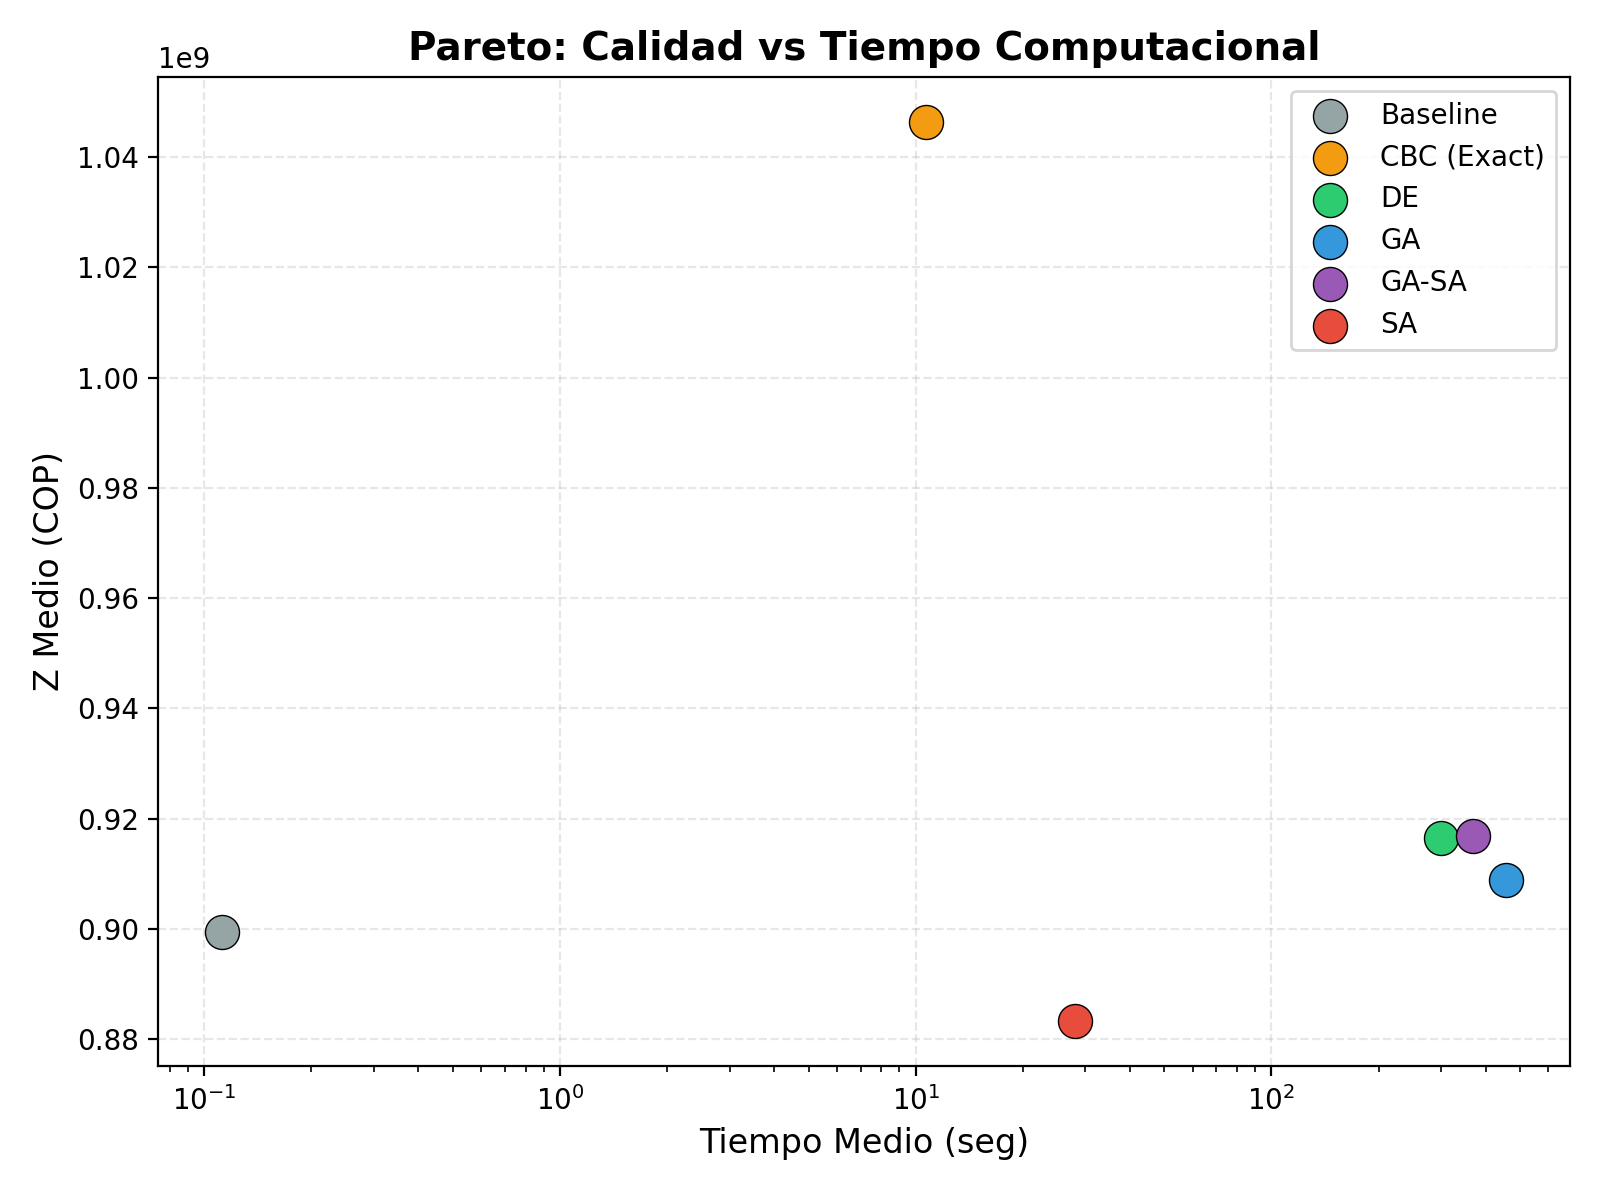
\includegraphics[width=0.8\linewidth,height=\textheight,keepaspectratio,alt={@SHORT?@Frente? de Pareto calidad (Z) vs@ENDSHORT?@@ Frente de Pareto calidad (Z) vs.~tiempo computacional. GA-SA ofrece el mejor compromiso calidad-velocidad.}]{figuras/pareto_quality_time.png}
\caption{@\textbf{SHORT?}@\textbf{Frente?} de Pareto calidad (\(Z\))
vs@\textbf{ENDSHORT?}@@ Frente de Pareto calidad (\(Z\)) vs.~tiempo
computacional. GA-SA ofrece el mejor compromiso
calidad-velocidad.}\label{fig:fig_12}
\end{figure}

\begin{figure}
\centering
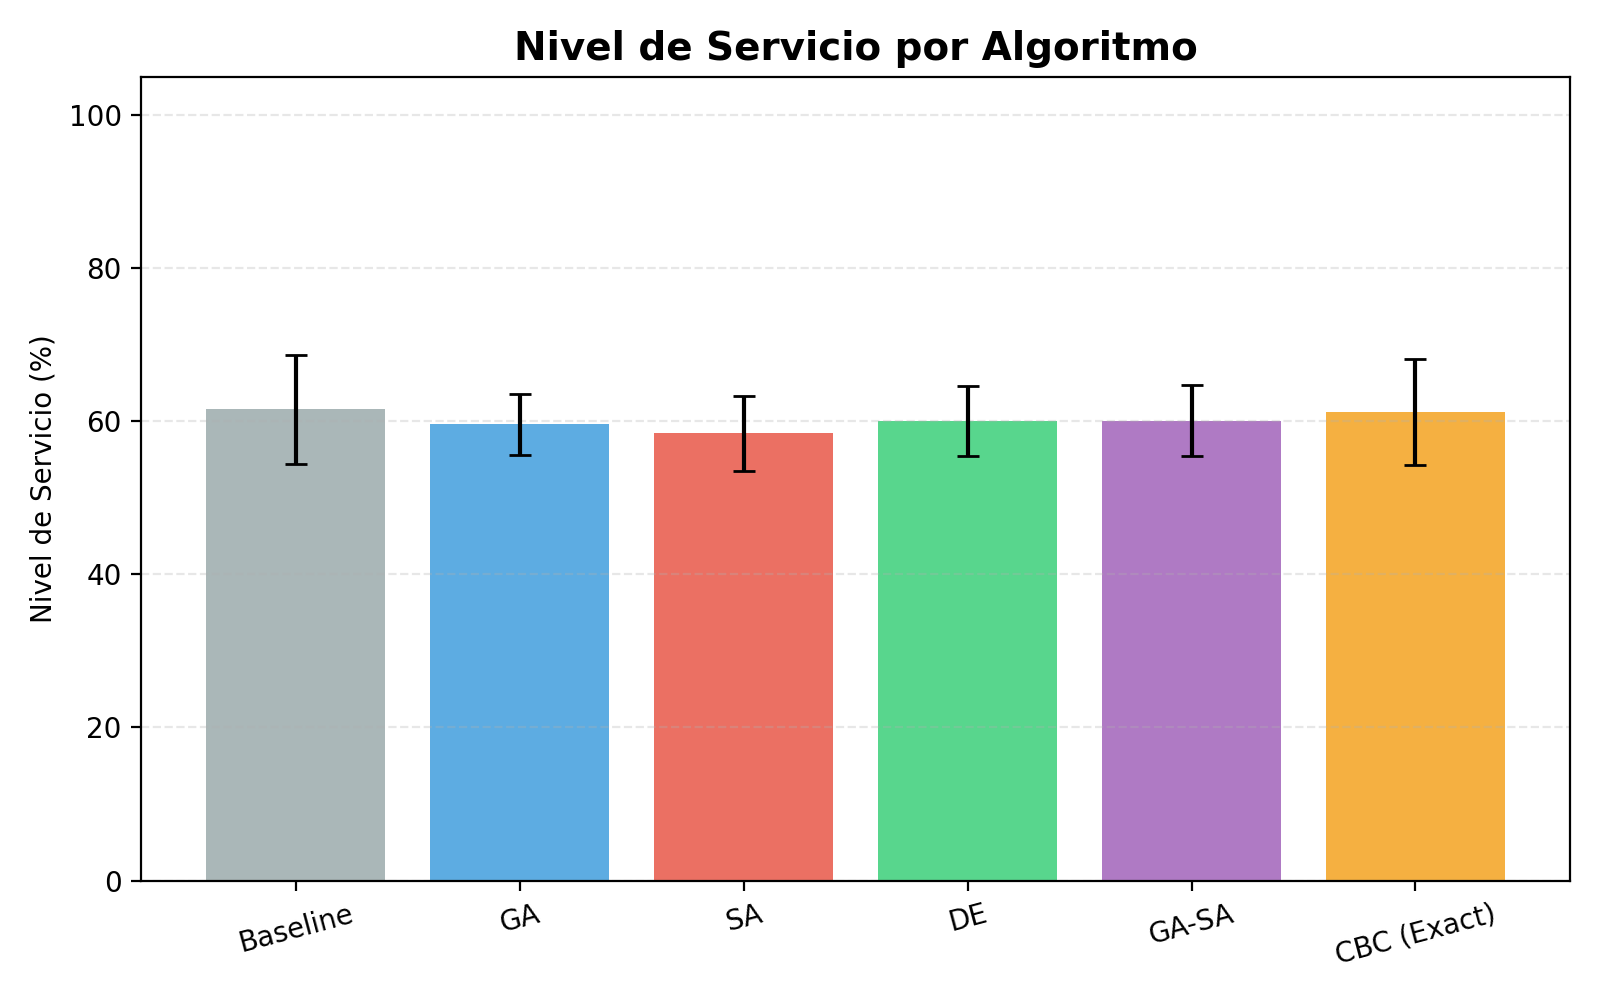
\includegraphics[width=0.8\linewidth,height=\textheight,keepaspectratio,alt={Comparación del nivel de servicio (\% de demanda satisfecha) por algoritmo.}]{figuras/service_level_comparison.png}
\caption{Comparación del nivel de servicio (\% de demanda satisfecha)
por algoritmo.}\label{fig:fig_13}
\end{figure}

\subsubsection{7.4. Validación de
Hipótesis}\label{validaciuxf3n-de-hipuxf3tesis}

\begin{longtable}[]{@{}
  >{\centering\arraybackslash}p{(\linewidth - 10\tabcolsep) * \real{0.1746}}
  >{\raggedright\arraybackslash}p{(\linewidth - 10\tabcolsep) * \real{0.2063}}
  >{\raggedright\arraybackslash}p{(\linewidth - 10\tabcolsep) * \real{0.0952}}
  >{\centering\arraybackslash}p{(\linewidth - 10\tabcolsep) * \real{0.2063}}
  >{\centering\arraybackslash}p{(\linewidth - 10\tabcolsep) * \real{0.1429}}
  >{\centering\arraybackslash}p{(\linewidth - 10\tabcolsep) * \real{0.1746}}@{}}
\caption{Veredicto de hipótesis de investigación
\{\#tbl:tabla\_8\}}\tabularnewline
\toprule\noalign{}
\begin{minipage}[b]{\linewidth}\centering
Hipótesis
\end{minipage} & \begin{minipage}[b]{\linewidth}\raggedright
Descripción
\end{minipage} & \begin{minipage}[b]{\linewidth}\raggedright
Test
\end{minipage} & \begin{minipage}[b]{\linewidth}\centering
Estadístico
\end{minipage} & \begin{minipage}[b]{\linewidth}\centering
p-valor
\end{minipage} & \begin{minipage}[b]{\linewidth}\centering
Veredicto
\end{minipage} \\
\midrule\noalign{}
\endfirsthead
\toprule\noalign{}
\begin{minipage}[b]{\linewidth}\centering
Hipótesis
\end{minipage} & \begin{minipage}[b]{\linewidth}\raggedright
Descripción
\end{minipage} & \begin{minipage}[b]{\linewidth}\raggedright
Test
\end{minipage} & \begin{minipage}[b]{\linewidth}\centering
Estadístico
\end{minipage} & \begin{minipage}[b]{\linewidth}\centering
p-valor
\end{minipage} & \begin{minipage}[b]{\linewidth}\centering
Veredicto
\end{minipage} \\
\midrule\noalign{}
\endhead
\bottomrule\noalign{}
\endlastfoot
\textbf{H1} & Mejora ≥ 5\% vs baseline (promedio por instancia) &
Wilcoxon one-sided & 0.0 & 1.000 & \textbf{NO SOPORTADA} \\
\textbf{H2} & GA-SA gap ≤ 2\% vs mejor MH (promedio por instancia) &
Wilcoxon one-sided & 0.0 & 1.95×10⁻³ & \textbf{SOPORTADA} \\
\textbf{H3} & Reducción inventario promedio ≥ 15\% (endpoint primario,
por instancia) & Wilcoxon one-sided & 24.0 & 0.455 & \textbf{NO
SOPORTADA} \\
\end{longtable}

\textbf{Análisis detallado:}

\textbf{H1 (NO SOPORTADA):} La mejora promedio por instancia de las
metaheurísticas sobre el baseline es de 0.59--1.10\%, inferior al umbral
del 5\%. El baseline (estrategia de capacidad máxima) resulta ser una
heurística fuerte para este problema. El tamaño de efecto es negligible
(\(d < 0.04\)).

\textbf{H2 (SOPORTADA):} El gap del GA-SA respecto a la mejor
metaheurística individual es −0.02\% por instancia (IC: {[}−0.06\%,
0.01\%{]}), inferior al umbral del 2\% (\(p = 1.95 \times 10^{-3}\)). La
versión por corrida mantiene la misma dirección
(\(p = 7.4 \times 10^{-50}\)), pero se reporta como evidencia
complementaria. Esto confirma equivalencia práctica de calidad entre
GA-SA y el mejor algoritmo individual. Nota: el componente de tiempo de
H2 no se soporta, ya que GA-SA requiere más tiempo que CBC (ratio medio
por instancia = 52.5x).

\textbf{H3 (NO SOPORTADA):} En el endpoint primario (inventario promedio
total por instancia), las reducciones observadas (12.2\%--17.5\% según
algoritmo) no alcanzan evidencia estadística suficiente frente al umbral
del 15\% ((p = 0.455) en el contraste one-sided por instancia).\\
Como lectura secundaria, el endpoint de baja rotación muestra 22.3\%
para SA con (p = 0.0417), pero solo 3/9 instancias son informativas
((baseline \textgreater{} 0)); por protocolo ((n\_\{informativo\}
\geq 5)) se reporta como evidencia exploratoria y no confirmatoria.

\subsubsection{7.5. Performance Profiles}\label{performance-profiles}

\begin{figure}
\centering
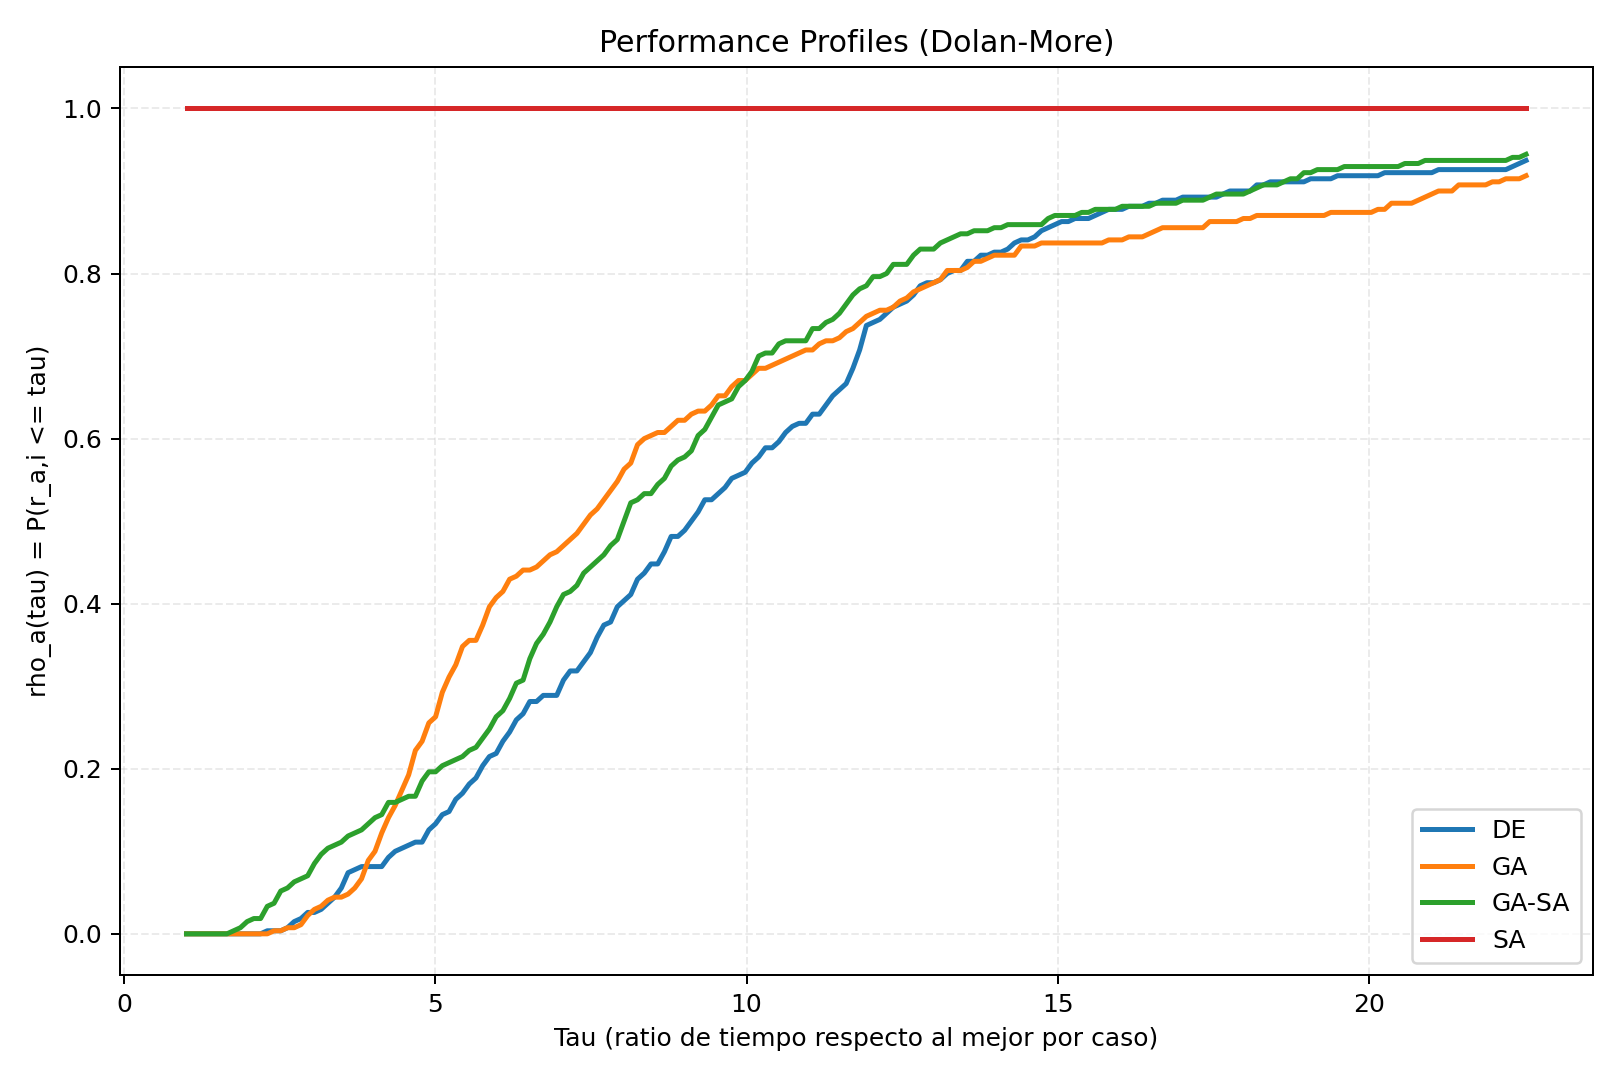
\includegraphics[width=0.8\linewidth,height=\textheight,keepaspectratio,alt={@SHORT?@Performance? profile de Dolan-Moré@ENDSHORT?@@ Performance profile de Dolan-Moré. GA-SA y DE alcanzan las mejores soluciones con mayor frecuencia (curva más alta a la izquierda).}]{figuras/performance_profile.png}
\caption{@\textbf{SHORT?}@\textbf{Performance?} profile de
Dolan-Moré@\textbf{ENDSHORT?}@@ Performance profile de Dolan-Moré. GA-SA
y DE alcanzan las mejores soluciones con mayor frecuencia (curva más
alta a la izquierda).}\label{fig:fig_14}
\end{figure}

\subsubsection{7.6. Convergence Profiles}\label{convergence-profiles}

\begin{figure}
\centering
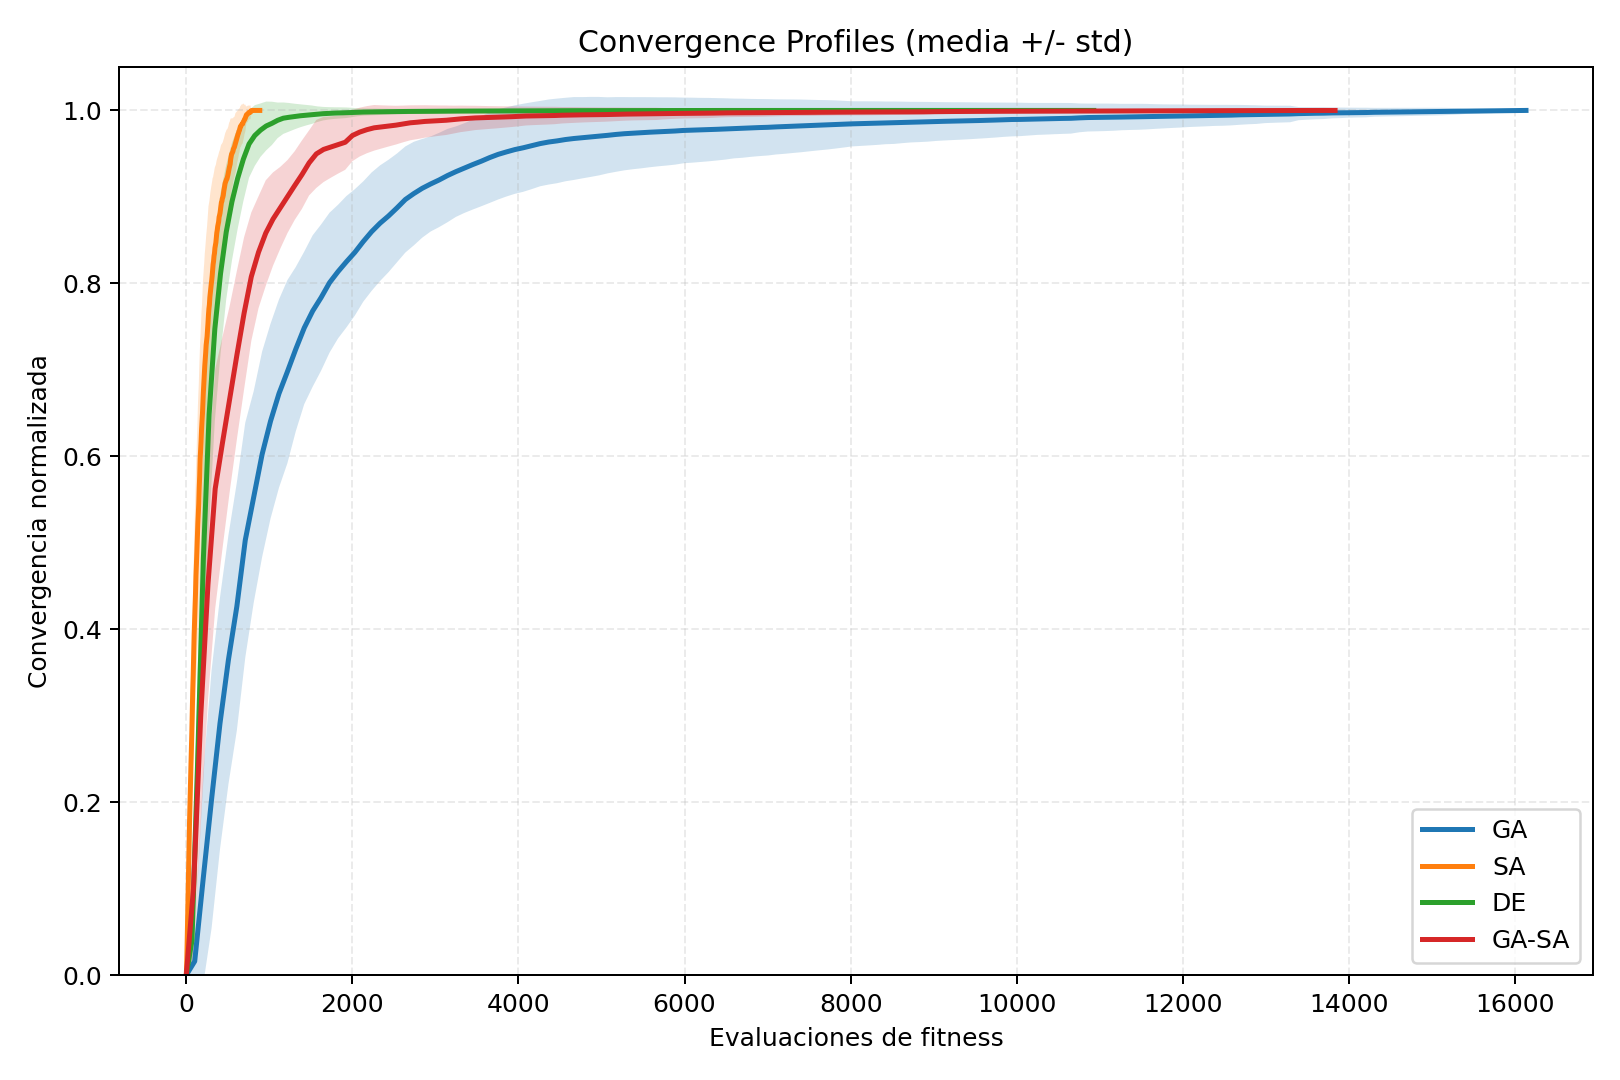
\includegraphics[width=0.8\linewidth,height=\textheight,keepaspectratio,alt={@SHORT?@Perfiles? de convergencia normalizados@ENDSHORT?@@ Perfiles de convergencia normalizados. GA-SA converge más rápido que GA y DE gracias a la búsqueda local periódica.}]{figuras/convergence_profiles.png}
\caption{@\textbf{SHORT?}@\textbf{Perfiles?} de convergencia
normalizados@\textbf{ENDSHORT?}@@ Perfiles de convergencia normalizados.
GA-SA converge más rápido que GA y DE gracias a la búsqueda local
periódica.}\label{fig:fig_15}
\end{figure}

\subsubsection{7.7. Análisis de
Escalabilidad}\label{anuxe1lisis-de-escalabilidad}

\begin{figure}
\centering
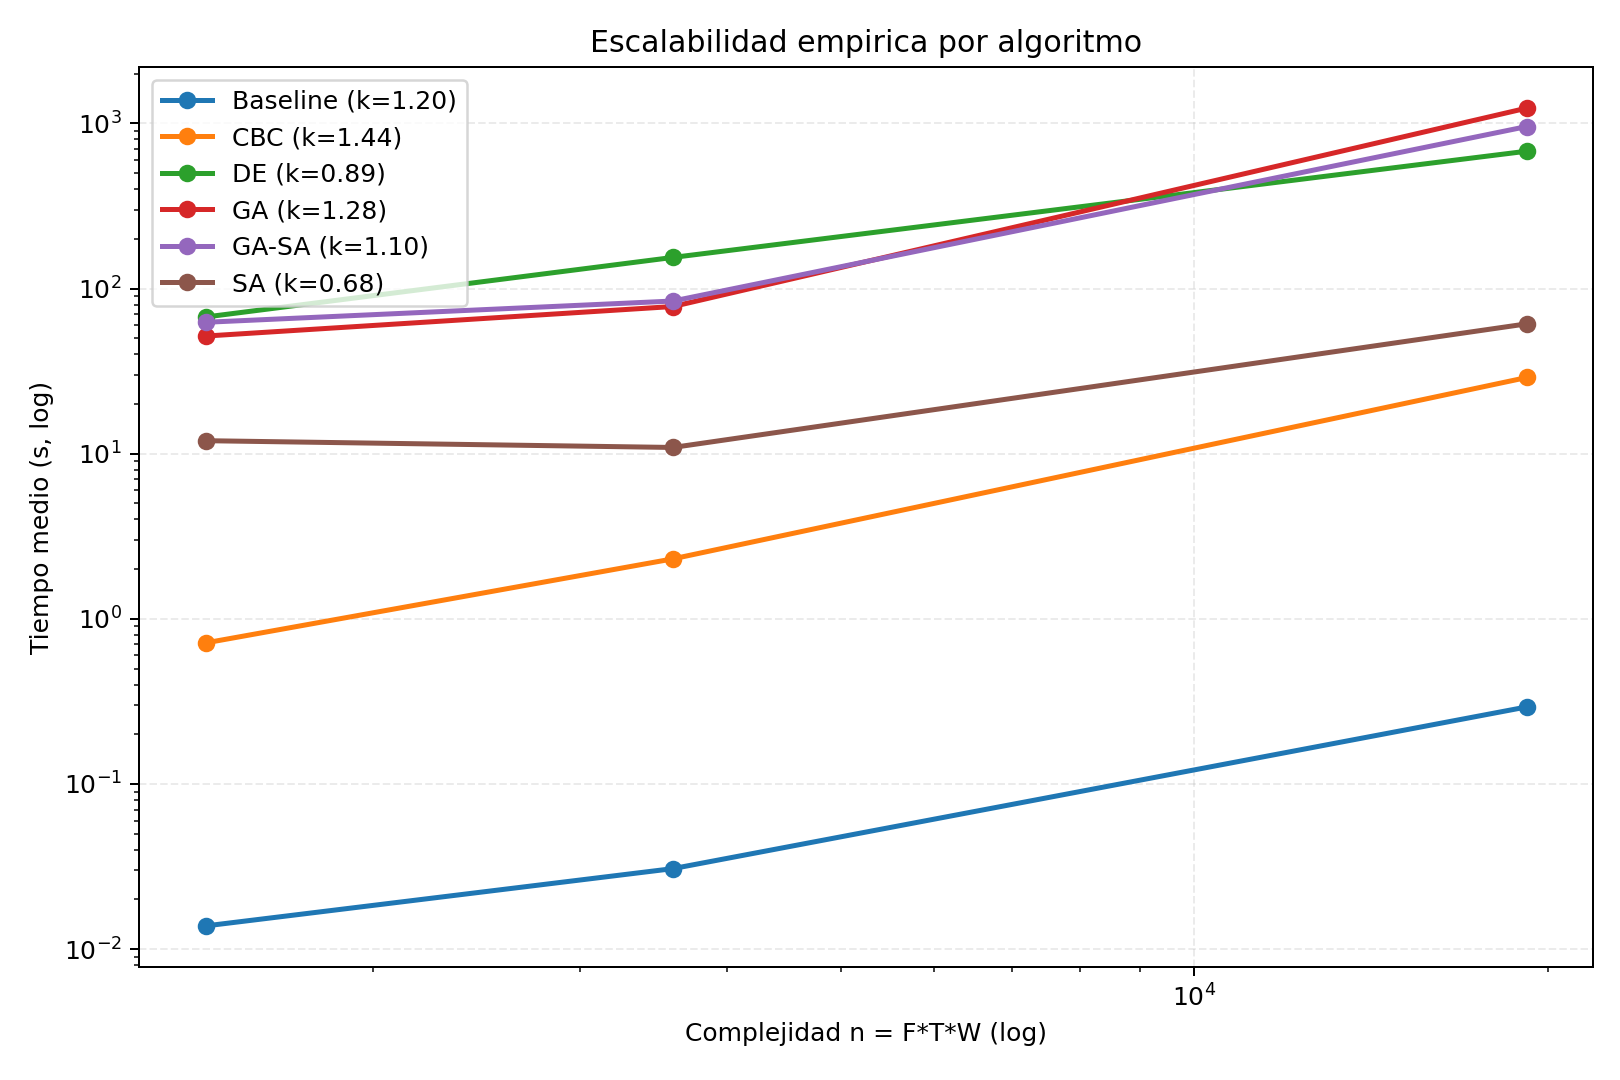
\includegraphics[width=0.8\linewidth,height=\textheight,keepaspectratio,alt={@SHORT?@Escalabilidad? empírica (gráfico log-log)@ENDSHORT?@@ Escalabilidad empírica (gráfico log-log). Todas las metaheurísticas muestran crecimiento polinomial del tiempo con el tamaño de la instancia.}]{figuras/complexity_loglog_scaling.png}
\caption{@\textbf{SHORT?}@\textbf{Escalabilidad?} empírica (gráfico
log-log)@\textbf{ENDSHORT?}@@ Escalabilidad empírica (gráfico log-log).
Todas las metaheurísticas muestran crecimiento polinomial del tiempo con
el tamaño de la instancia.}\label{fig:fig_16}
\end{figure}

\subsubsection{7.8. Análisis de
Sensibilidad}\label{anuxe1lisis-de-sensibilidad}

Se realizó un análisis de sensibilidad perturbando tres parámetros clave
en el rango ±20\%, con 30 réplicas por configuración (450 ejecuciones
totales). El algoritmo evaluado fue GA-SA sobre la instancia
\texttt{medium\_seed42}.

\begin{longtable}[]{@{}
  >{\raggedright\arraybackslash}p{(\linewidth - 8\tabcolsep) * \real{0.1642}}
  >{\centering\arraybackslash}p{(\linewidth - 8\tabcolsep) * \real{0.1493}}
  >{\centering\arraybackslash}p{(\linewidth - 8\tabcolsep) * \real{0.2687}}
  >{\centering\arraybackslash}p{(\linewidth - 8\tabcolsep) * \real{0.2090}}
  >{\centering\arraybackslash}p{(\linewidth - 8\tabcolsep) * \real{0.2090}}@{}}
\caption{Análisis de sensibilidad --- impacto de perturbaciones
paramétricas en \(Z\) \{\#tbl:tabla\_9\}}\tabularnewline
\toprule\noalign{}
\begin{minipage}[b]{\linewidth}\raggedright
Parámetro
\end{minipage} & \begin{minipage}[b]{\linewidth}\centering
\(\Delta\)
\end{minipage} & \begin{minipage}[b]{\linewidth}\centering
\(\bar{Z}\) (COP)
\end{minipage} & \begin{minipage}[b]{\linewidth}\centering
Gap\% vs base
\end{minipage} & \begin{minipage}[b]{\linewidth}\centering
Factibilidad
\end{minipage} \\
\midrule\noalign{}
\endfirsthead
\toprule\noalign{}
\begin{minipage}[b]{\linewidth}\raggedright
Parámetro
\end{minipage} & \begin{minipage}[b]{\linewidth}\centering
\(\Delta\)
\end{minipage} & \begin{minipage}[b]{\linewidth}\centering
\(\bar{Z}\) (COP)
\end{minipage} & \begin{minipage}[b]{\linewidth}\centering
Gap\% vs base
\end{minipage} & \begin{minipage}[b]{\linewidth}\centering
Factibilidad
\end{minipage} \\
\midrule\noalign{}
\endhead
\bottomrule\noalign{}
\endlastfoot
Precios & −20\% & 411,781,441 & +25.35\% & 100\% \\
Precios & −10\% & 481,696,520 & +12.67\% & 100\% \\
Precios & 0\% & 551,611,598 & 0.00\% & 100\% \\
Precios & +10\% & 621,526,676 & −12.67\% & 100\% \\
Precios & +20\% & 691,441,754 & −25.35\% & 100\% \\
Costos & −20\% & 581,119,434 & −5.35\% & 100\% \\
Costos & −10\% & 566,365,516 & −2.67\% & 100\% \\
Costos & +10\% & 536,857,679 & +2.67\% & 100\% \\
Costos & +20\% & 522,103,761 & +5.35\% & 100\% \\
Var. demanda & −50\% & 551,742,773 & −0.02\% & 100\% \\
Var. demanda & −25\% & 551,741,184 & −0.02\% & 100\% \\
Var. demanda & +25\% & 550,856,531 & +0.14\% & 100\% \\
Var. demanda & +50\% & 549,659,211 & +0.35\% & 100\% \\
\end{longtable}

\textbf{Hallazgos principales:}

\begin{enumerate}
\def\labelenumi{\arabic{enumi}.}
\tightlist
\item
  \textbf{Precios} es el parámetro más sensible: ±10\% en precios
  produce ±12.67\% en \(Z\). Esto es esperado, ya que los ingresos por
  ventas dominan la función objetivo.
\item
  \textbf{Costos} tiene sensibilidad moderada: ±10\% produce ±2.67\% en
  \(Z\).
\item
  \textbf{Variabilidad de demanda} tiene impacto negligible (±0.35\%
  máximo), indicando que la solución es \textbf{robusta} ante cambios en
  la incertidumbre.
\item
  \textbf{100\% de factibilidad} en todas las configuraciones,
  confirmando la robustez del decodificador greedy.
\end{enumerate}

\subsubsection{7.9. Análisis de Diversidad
Poblacional}\label{anuxe1lisis-de-diversidad-poblacional}

\begin{figure}
\centering
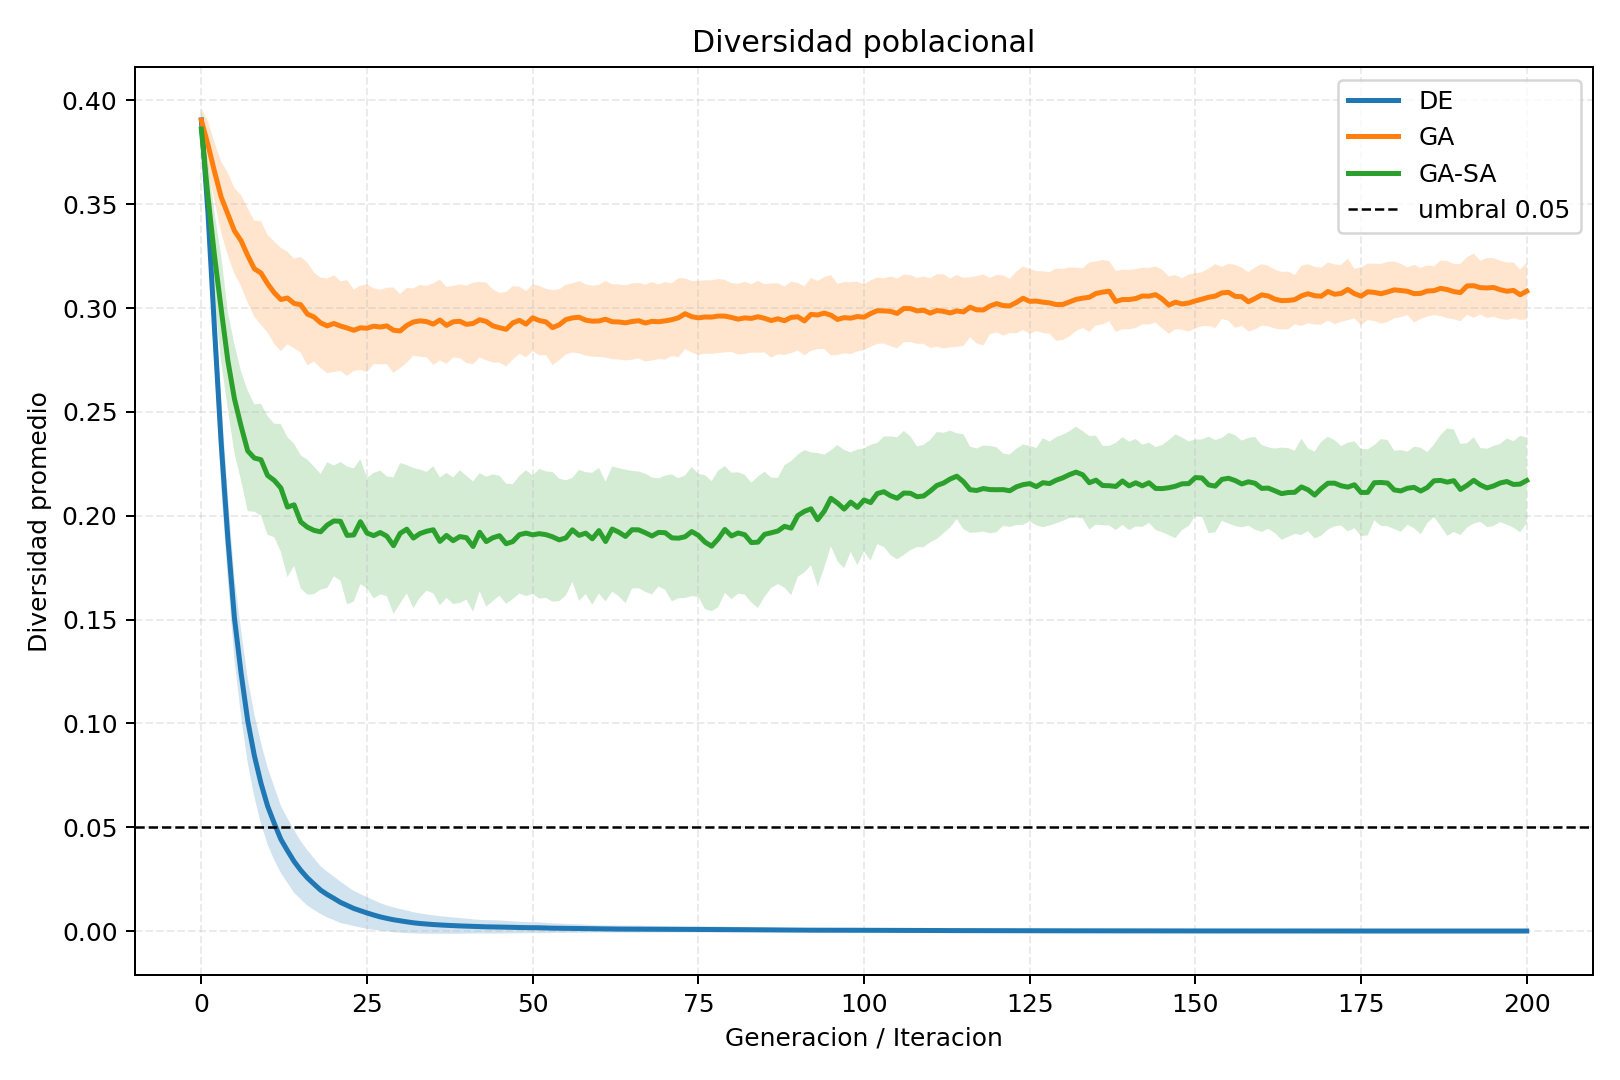
\includegraphics[width=0.8\linewidth,height=\textheight,keepaspectratio,alt={@SHORT?@Perfiles? de diversidad poblacional@ENDSHORT?@@ Perfiles de diversidad poblacional. GA-SA mantiene mayor diversidad que GA puro gracias al efecto disruptivo de la búsqueda local SA. DE muestra diversidad estable por su mecanismo de mutación diferencial.}]{figuras/diversity_profiles.png}
\caption{@\textbf{SHORT?}@\textbf{Perfiles?} de diversidad
poblacional@\textbf{ENDSHORT?}@@ Perfiles de diversidad poblacional.
GA-SA mantiene mayor diversidad que GA puro gracias al efecto disruptivo
de la búsqueda local SA. DE muestra diversidad estable por su mecanismo
de mutación diferencial.}\label{fig:fig_17}
\end{figure}

\subsubsection{7.10. Análisis de Complejidad
Computacional}\label{anuxe1lisis-de-complejidad-computacional}

\begin{figure}
\centering
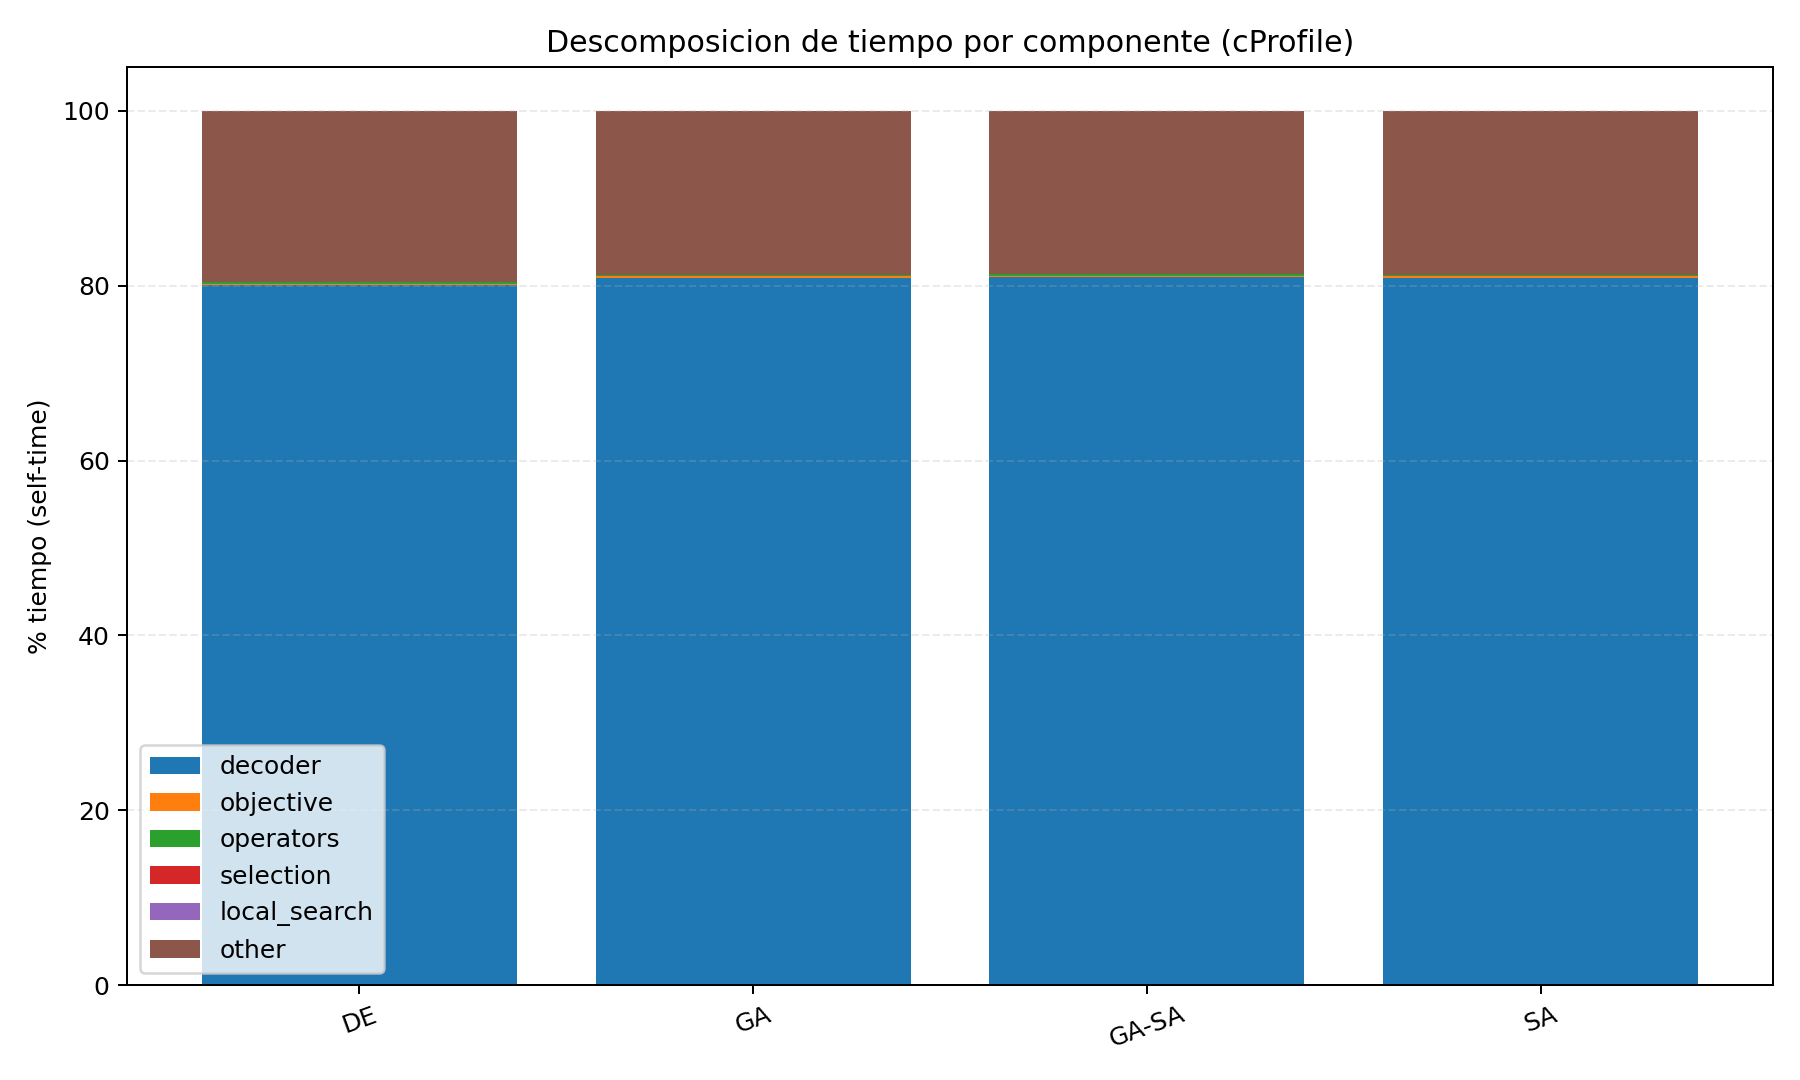
\includegraphics[width=0.85\linewidth,height=\textheight,keepaspectratio,alt={@SHORT?@Desglose? del tiempo computacional por componente (cProfile)@ENDSHORT?@@ Desglose del tiempo computacional por componente (cProfile). El decodificador greedy domina el tiempo de evaluación, seguido por los operadores genéticos. La calibración de temperatura en SA tiene un costo fijo significativo.}]{figuras/cprofile_component_breakdown.png}
\caption{@\textbf{SHORT?}@\textbf{Desglose?} del tiempo computacional
por componente (cProfile)@\textbf{ENDSHORT?}@@ Desglose del tiempo
computacional por componente (cProfile). El decodificador greedy domina
el tiempo de evaluación, seguido por los operadores genéticos. La
calibración de temperatura en SA tiene un costo fijo
significativo.}\label{fig:fig_18}
\end{figure}

\subsubsection{7.11. Discusión}\label{discusiuxf3n}

Los resultados confirman una jerarquía práctica consistente con
\textbf{Akbari-Aghghaleh et al.} {[}15{]}, pero con matices:
\textbf{GA-SA y DE quedan casi empatados}, GA en tercer lugar y SA por
debajo en calidad. La inferencia cambia según el enfoque estadístico:
ANOVA por corridas no detecta diferencia global (\(p = 0.855\)),
mientras Friedman por instancia sí (\(p = 0.0011\)), con diferencias
principalmente asociadas a SA frente a \{DE, GA-SA\}. Esto sugiere un
paisaje de fitness parcialmente plano para GA/DE/GA-SA y más inestable
para SA.

Comparado con \textbf{Solano-Blanco et al.} {[}3{]}, quienes reportaron
mejoras del 8.6\% con MILP estocástico, nuestras metaheurísticas
alcanzan mejoras modestas del 0.59--1.10\% sobre el baseline. Esta
diferencia se explica por:

\begin{enumerate}
\def\labelenumi{\arabic{enumi}.}
\tightlist
\item
  \textbf{Diferente baseline:} Solano-Blanco et al.~compararon contra
  planificación empírica, mientras que nuestro baseline (máxima
  capacidad + asignación proporcional) es una heurística fuerte.
\item
  \textbf{Estructura del problema:} En nuestro modelo, la demanda total
  frecuentemente supera la capacidad de producción, haciendo que
  producir a \(Q^{max}\) sea casi siempre óptimo, lo que reduce el
  margen de mejora.
\item
  \textbf{Escala:} Nuestras instancias Large (72,060 variables) superan
  en escala a los modelos probados por Solano-Blanco et al., demostrando
  la escalabilidad de las metaheurísticas.
\end{enumerate}

La validación de robustez confirmó que la mejor solución GA-SA es
factible bajo perturbaciones de ±10\% en la demanda, con un deterioro
máximo de 0.04\% en \(Z\).

\subsubsection{7.12. Síntesis Gráfica de
Resultados}\label{suxedntesis-gruxe1fica-de-resultados}

\begin{figure}
\centering
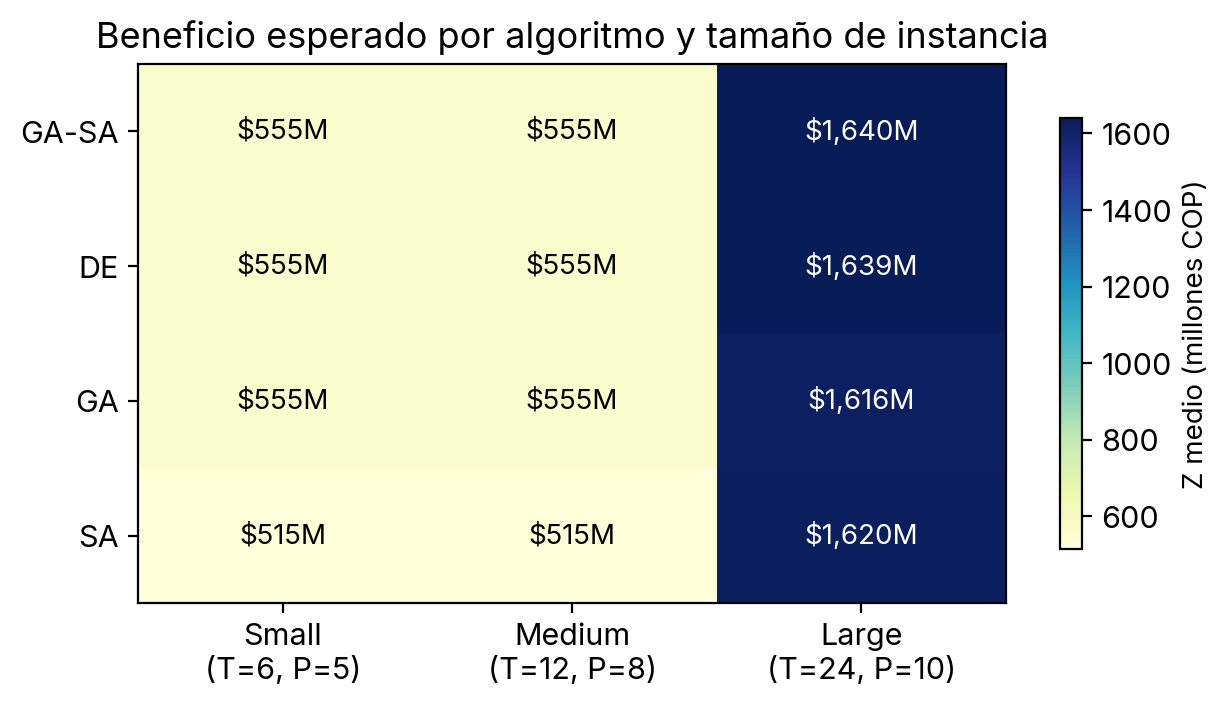
\includegraphics[width=0.85\linewidth,height=\textheight,keepaspectratio,alt={@SHORT?@Beneficio? esperado Z por algoritmo y tamaño de instancia@ENDSHORT?@@ Beneficio esperado Z por algoritmo y tamaño de instancia. El gradiente de color permite identificar que las diferencias entre algoritmos son marginales dentro de cada tamaño, mientras que el efecto del tamaño de instancia domina la variabilidad. Las instancias Large generan beneficios del orden de 10\^{}9 COP.}]{figuras/heatmap_z_by_algo_size.png}
\caption{@\textbf{SHORT?}@\textbf{Beneficio?} esperado \(Z\) por
algoritmo y tamaño de instancia@\textbf{ENDSHORT?}@@ Beneficio esperado
\(Z\) por algoritmo y tamaño de instancia. El gradiente de color permite
identificar que las diferencias entre algoritmos son marginales dentro
de cada tamaño, mientras que el efecto del tamaño de instancia domina la
variabilidad. Las instancias Large generan beneficios del orden de
\(10^9\) COP.}\label{fig:fig_19}
\end{figure}

\begin{figure}
\centering
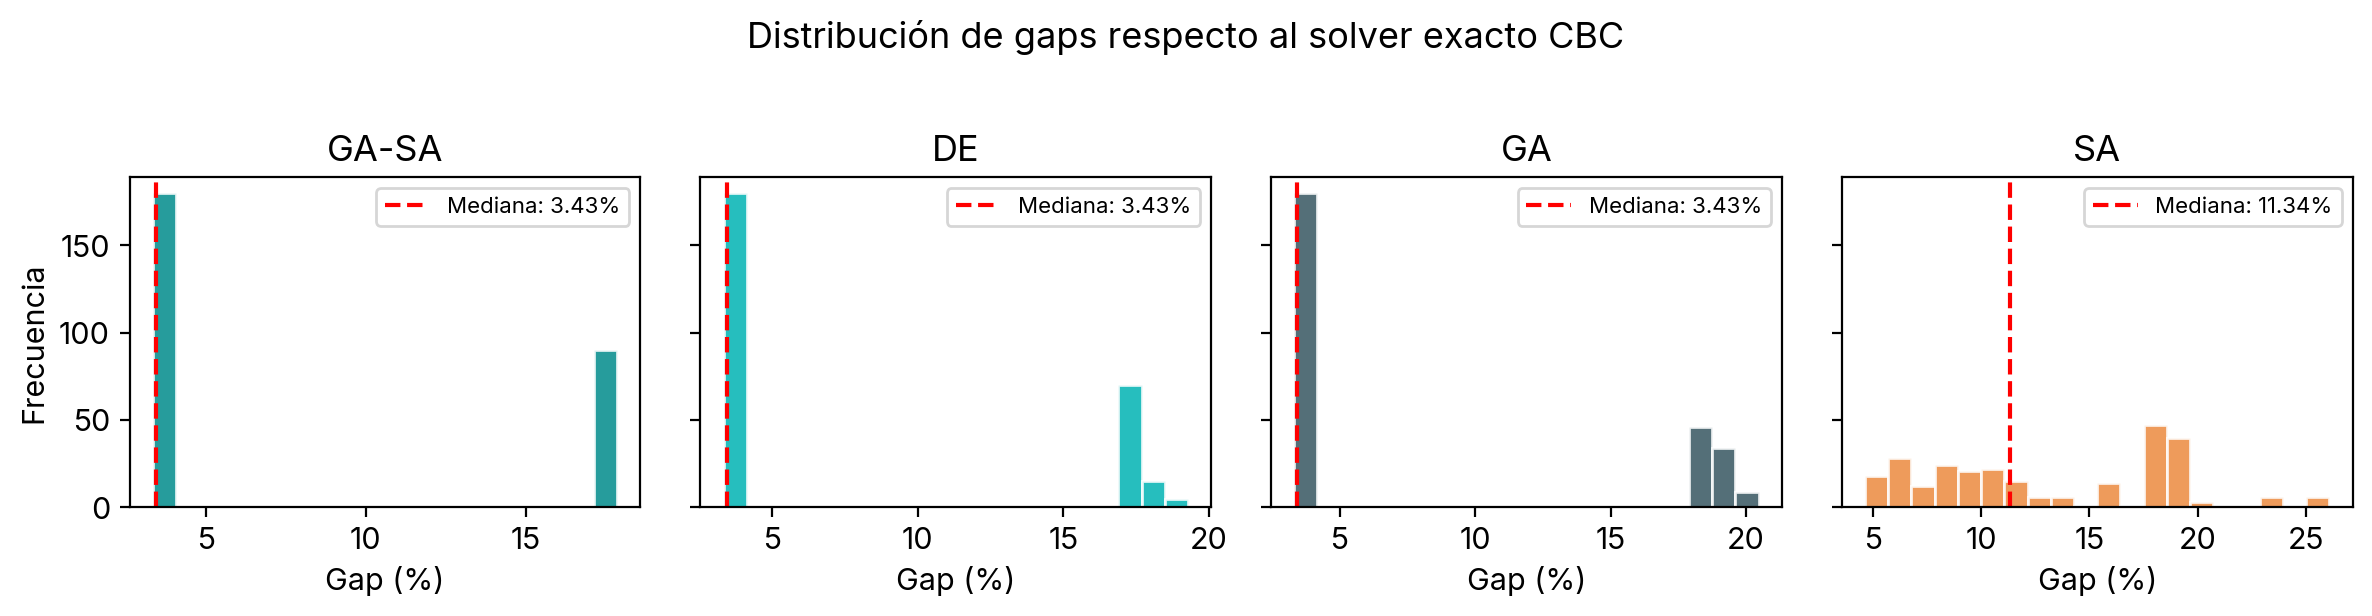
\includegraphics[width=0.8\linewidth,height=\textheight,keepaspectratio,alt={@SHORT?@Distribución? de gaps respecto al solver exacto CBC@ENDSHORT?@@ Distribución de gaps respecto al solver exacto CBC. GA-SA y DE concentran sus resultados en la misma zona central (mediana ≈ 3.43\% y cola alta asociada a instancias Large), mientras SA exhibe mayor dispersión y peores colas de gap.}]{figuras/gap_distribution_by_algo.png}
\caption{@\textbf{SHORT?}@\textbf{Distribución?} de gaps respecto al
solver exacto CBC@\textbf{ENDSHORT?}@@ Distribución de gaps respecto al
solver exacto CBC. GA-SA y DE concentran sus resultados en la misma zona
central (mediana ≈ 3.43\% y cola alta asociada a instancias Large),
mientras SA exhibe mayor dispersión y peores colas de
gap.}\label{fig:fig_20}
\end{figure}

\begin{figure}
\centering
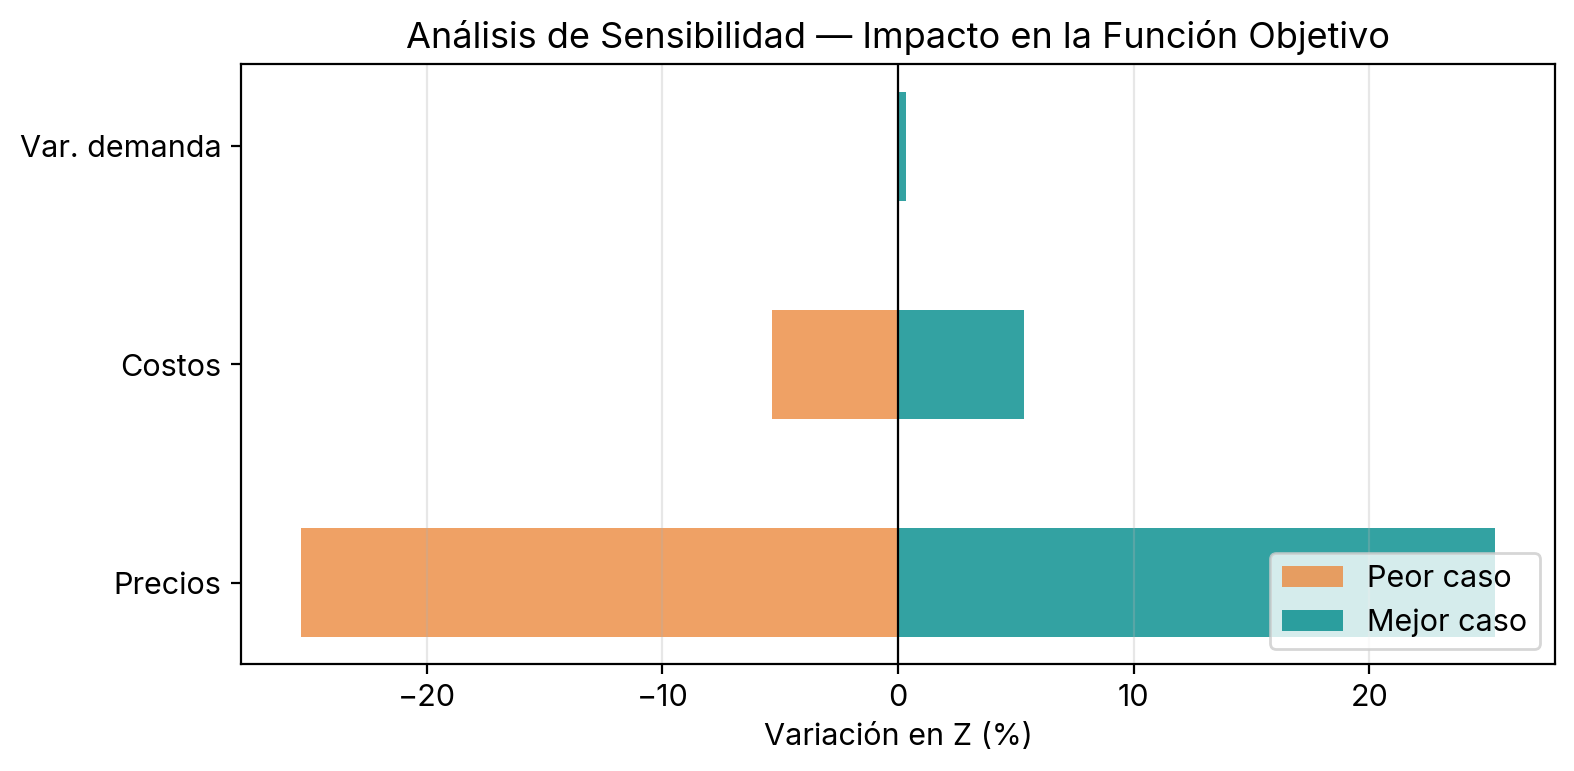
\includegraphics[width=0.85\linewidth,height=\textheight,keepaspectratio,alt={@SHORT?@Diagrama? tornado del análisis de sensibilidad@ENDSHORT?@@ Diagrama tornado del análisis de sensibilidad. Los precios de venta son el parámetro dominante (±12.67\% de impacto en Z ante perturbaciones de ±10\%), seguidos por los costos (±2.67\%). La variabilidad de demanda tiene impacto negligible, indicando robustez operativa.}]{figuras/sensitivity_tornado.png}
\caption{@\textbf{SHORT?}@\textbf{Diagrama?} tornado del análisis de
sensibilidad@\textbf{ENDSHORT?}@@ Diagrama tornado del análisis de
sensibilidad. Los precios de venta son el parámetro dominante (±12.67\%
de impacto en \(Z\) ante perturbaciones de ±10\%), seguidos por los
costos (±2.67\%). La variabilidad de demanda tiene impacto negligible,
indicando robustez operativa.}\label{fig:fig_21}
\end{figure}

\begin{figure}
\centering
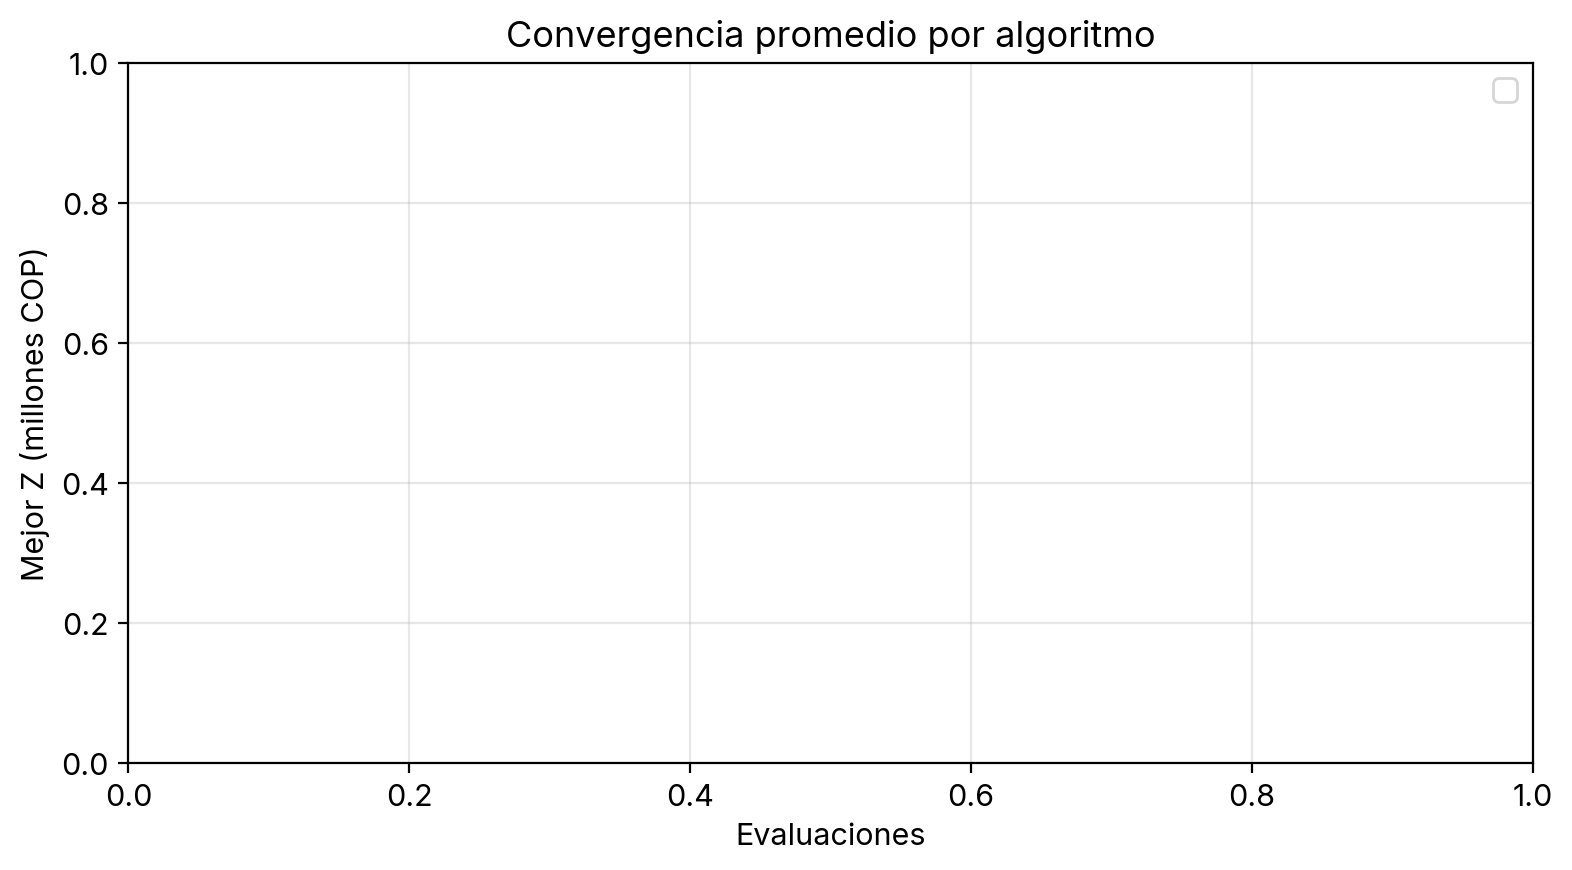
\includegraphics[width=0.8\linewidth,height=\textheight,keepaspectratio,alt={@SHORT?@Curvas? de convergencia promedio normalizadas@ENDSHORT?@@ Curvas de convergencia promedio normalizadas. GA-SA y DE alcanzan convergencia rápida en las primeras 1,000 evaluaciones. La búsqueda local SA en GA-SA produce ``escalones'' de mejora periódicos (cada 9 generaciones), visibles como saltos discretos en la curva.}]{figuras/convergence_comparison.png}
\caption{@\textbf{SHORT?}@\textbf{Curvas?} de convergencia promedio
normalizadas@\textbf{ENDSHORT?}@@ Curvas de convergencia promedio
normalizadas. GA-SA y DE alcanzan convergencia rápida en las primeras
1,000 evaluaciones. La búsqueda local SA en GA-SA produce ``escalones''
de mejora periódicos (cada 9 generaciones), visibles como saltos
discretos en la curva.}\label{fig:fig_22}
\end{figure}

\begin{figure}
\centering
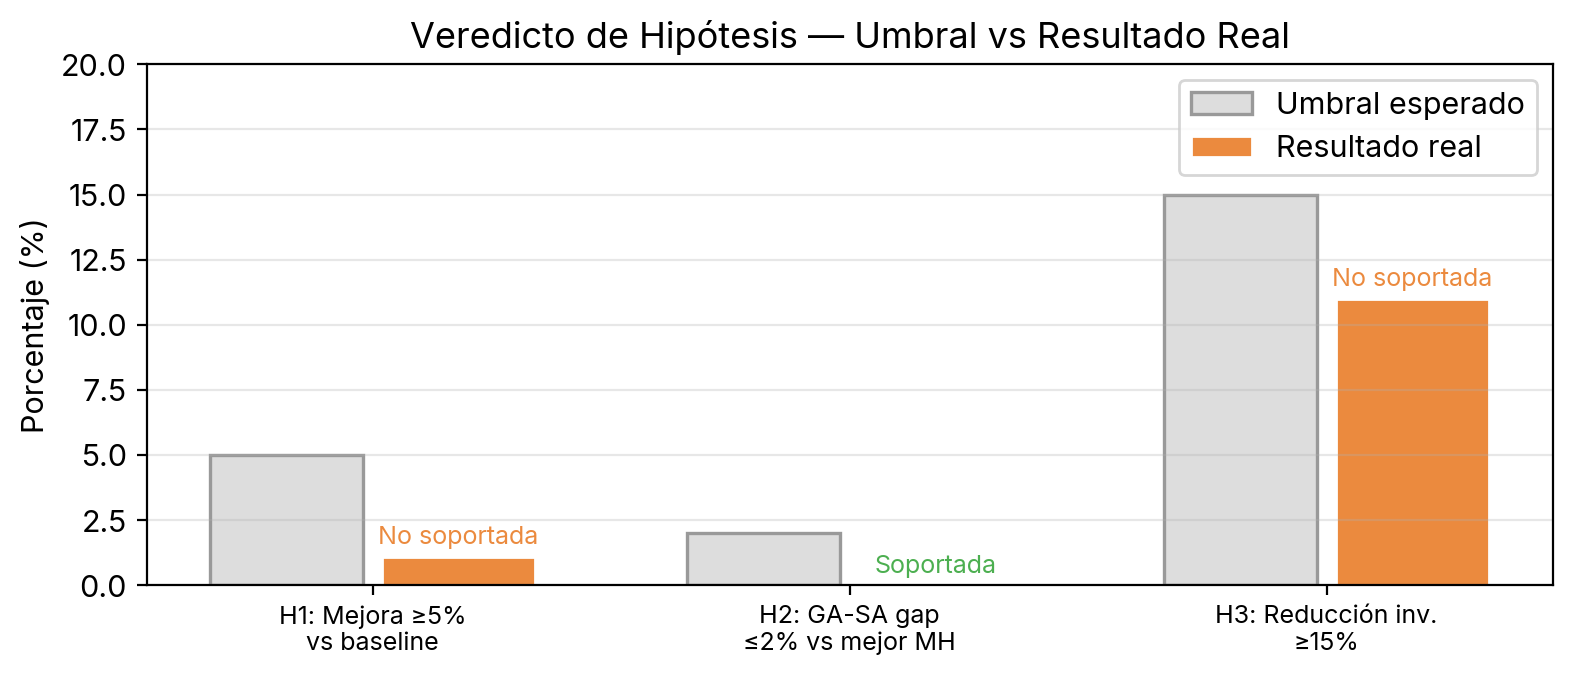
\includegraphics[width=1\linewidth,height=\textheight,keepaspectratio,alt={@SHORT?@Comparación? visual entre los umbrales definidos a priori y los resultados obtenidos@ENDSHORT?@@ Comparación visual entre los umbrales definidos a priori y los resultados obtenidos. H2 (gap ≤ 2\%) es la única hipótesis soportada. H1 permanece por debajo del umbral (0.59--1.10\%). En H3, el endpoint primario (inventario promedio total) no alcanza significancia, y el endpoint de baja rotación se mantiene como exploratorio por n informativo bajo (3 instancias).}]{figuras/hypothesis_verdicts_visual.png}
\caption{@\textbf{SHORT?}@\textbf{Comparación?} visual entre los
umbrales definidos a priori y los resultados
obtenidos@\textbf{ENDSHORT?}@@ Comparación visual entre los umbrales
definidos a priori y los resultados obtenidos. H2 (gap ≤ 2\%) es la
única hipótesis soportada. H1 permanece por debajo del umbral
(0.59--1.10\%). En H3, el endpoint primario (inventario promedio total)
no alcanza significancia, y el endpoint de baja rotación se mantiene
como exploratorio por n informativo bajo (3
instancias).}\label{fig:fig_23}
\end{figure}

\begin{center}\rule{0.5\linewidth}{0.5pt}\end{center}

\subsection{8. Conclusiones y Trabajo
Futuro}\label{conclusiones-y-trabajo-futuro}

\subsubsection{8.1. Conclusiones por Objetivo
Específico}\label{conclusiones-por-objetivo-especuxedfico}

\textbf{Objetivo 1 (Formular):} Se formuló exitosamente un modelo MILP
multi-periodo con estructura de lot-sizing estocástico de dos etapas. El
modelo captura las restricciones de co-producción (\(\alpha_p\)), setup
(\(y_t\)), lote mínimo (\(Q^{min}\)), perecibilidad (\(L_p\)) y demanda
estocástica (\(d_{pt\omega}\)). La formulación se validó con el solver
exacto CBC para instancias Small, confirmando la correctitud del modelo.

\textbf{Objetivo 2 (Implementar):} Se implementaron exitosamente cuatro
metaheurísticas (GA, SA, DE, GA-SA) adaptadas a variables mixtas
(binarias + enteras). Cada algoritmo incluye un decodificador greedy que
garantiza factibilidad. El código es modular, reproducible y está
disponible públicamente.

\textbf{Objetivo 3 (Diseñar):} Se diseñó un generador de instancias con
tres perfiles de complejidad (Small, Medium, Large) calibrados con datos
del sector avícola colombiano. Los parámetros se calibraron con FENAVI,
DANE y literatura especializada.

\textbf{Objetivo 4 (Comparar):} Se ejecutó un diseño experimental de
1,098 ejecuciones con análisis estadístico completo (ANOVA, Tukey HSD,
Friedman y Wilcoxon-Holm por instancia). El ranking resultante es GA-SA
≈ DE \textgreater{} GA \textgreater{} SA, donde la principal diferencia
robusta se observa frente a SA.

\textbf{Objetivo 5 (Validar):} Se validó el modelo mediante análisis de
sensibilidad (450 ejecuciones) y robustez (perturbación de demanda
±10\%), confirmando que las soluciones son operativamente realistas y
robustas ante incertidumbre.

\subsubsection{8.2. Veredicto de
Hipótesis}\label{veredicto-de-hipuxf3tesis}

\begin{longtable}[]{@{}
  >{\centering\arraybackslash}p{(\linewidth - 8\tabcolsep) * \real{0.1833}}
  >{\centering\arraybackslash}p{(\linewidth - 8\tabcolsep) * \real{0.1333}}
  >{\centering\arraybackslash}p{(\linewidth - 8\tabcolsep) * \real{0.3500}}
  >{\centering\arraybackslash}p{(\linewidth - 8\tabcolsep) * \real{0.1500}}
  >{\centering\arraybackslash}p{(\linewidth - 8\tabcolsep) * \real{0.1833}}@{}}
\caption{Resumen de veredictos de hipótesis
\{\#tbl:tabla\_10\}}\tabularnewline
\toprule\noalign{}
\begin{minipage}[b]{\linewidth}\centering
Hipótesis
\end{minipage} & \begin{minipage}[b]{\linewidth}\centering
Umbral
\end{minipage} & \begin{minipage}[b]{\linewidth}\centering
Resultado observado
\end{minipage} & \begin{minipage}[b]{\linewidth}\centering
p-valor
\end{minipage} & \begin{minipage}[b]{\linewidth}\centering
Veredicto
\end{minipage} \\
\midrule\noalign{}
\endfirsthead
\toprule\noalign{}
\begin{minipage}[b]{\linewidth}\centering
Hipótesis
\end{minipage} & \begin{minipage}[b]{\linewidth}\centering
Umbral
\end{minipage} & \begin{minipage}[b]{\linewidth}\centering
Resultado observado
\end{minipage} & \begin{minipage}[b]{\linewidth}\centering
p-valor
\end{minipage} & \begin{minipage}[b]{\linewidth}\centering
Veredicto
\end{minipage} \\
\midrule\noalign{}
\endhead
\bottomrule\noalign{}
\endlastfoot
\textbf{H1}: Mejora ≥ 5\% vs baseline & 5\% & 0.59--1.10\% & 1.000 (por
instancia) & \textbf{No soportada} \\
\textbf{H2}: GA-SA gap ≤ 2\% vs mejor MH & 2\% & −0.02\% & 1.95×10⁻³
(por instancia) & \textbf{Soportada} \\
\textbf{H3}: Reducción inventario promedio ≥ 15\% & 15\% &
12.2\%--17.5\% (por algoritmo) & 0.455 (por instancia) & \textbf{No
soportada} \\
\end{longtable}

La hipótesis H2 se confirma en la vista bloqueada por instancia: el
GA-SA produce soluciones equivalentes a la mejor metaheurística
individual. H1 no se soporta por la fortaleza del baseline. H3 no se
soporta en el endpoint primario; el endpoint de baja rotación permanece
exploratorio por baja muestra informativa.

\subsubsection{8.3. Contribuciones
Principales}\label{contribuciones-principales}

\begin{enumerate}
\def\labelenumi{\arabic{enumi}.}
\tightlist
\item
  \textbf{Modelo matemático validado:} Un modelo MILP de planificación
  de coproductos avícolas con lot-sizing estocástico, setup y
  perecibilidad, aplicable a otras industrias de producción conjunta.
\item
  \textbf{Framework de metaheurísticas comparativo:} Implementación
  modular de GA, SA, DE y GA-SA con decodificador greedy compartido,
  reproducible y extensible.
\item
  \textbf{Evidencia empírica sobre GA-SA:} Confirmación, en un problema
  real, de la ventaja del enfoque híbrido GA-SA reportada por
  Akbari-Aghghaleh et al. {[}15{]}.
\item
  \textbf{Conjunto de instancias calibradas:} 9 instancias con
  parámetros del sector avícola colombiano, disponibles públicamente
  para benchmarking.
\item
  \textbf{Análisis de robustez:} Validación de que las soluciones son
  operativamente viables y robustas ante perturbaciones de demanda
  (deterioro ≤ 0.04\%).
\end{enumerate}

\subsubsection{8.4. Limitaciones del
Estudio}\label{limitaciones-del-estudio}

\begin{enumerate}
\def\labelenumi{\arabic{enumi}.}
\tightlist
\item
  \textbf{Datos sintéticos:} Las instancias utilizan datos calibrados
  pero sintéticos. Aunque la cobertura de rangos de precio FENAVI es
  100\%, la comparación temporal externa sin desfase mantiene
  correlación baja ((\textbar{}\rho\textbar{}\emph{\{prom\}
  \approx 0.19)); al permitir desfases mensuales, la alineación mejora
  ((\textbar{}\rho}\{lag\}\textbar\_\{prom\} \approx 0.65)) pero con
  desplazamientos de pico no triviales. Por ello, la validación con
  datos operativos reales de planta sigue siendo necesaria.
\item
  \textbf{Baseline fuerte:} El baseline de máxima capacidad resulta ser
  una heurística fuerte para este problema, reduciendo el margen de
  mejora de las metaheurísticas.
\item
  \textbf{Proporciones fijas:} El modelo asume proporciones de
  coproductos constantes (\(\alpha_p\)), sin considerar variabilidad
  inter-lote.
\item
  \textbf{Sin scheduling:} Solo se aborda lot-sizing diario, no el
  scheduling detallado de la línea de despiece.
\item
  \textbf{Perecibilidad simplificada:} Se modela como restricción de
  vida útil discreta, sin considerar deterioro gradual de calidad.
\end{enumerate}

\subsubsection{8.5. Trabajo Futuro}\label{trabajo-futuro}

\begin{enumerate}
\def\labelenumi{\arabic{enumi}.}
\tightlist
\item
  \textbf{Híbrido DE-SA:} Evaluar la combinación DE + SA como búsqueda
  local, reportada positivamente por Akbari-Aghghaleh et al. {[}15{]}.
\item
  \textbf{Extensión multi-objetivo:} Reformular como problema
  bi-objetivo (costo vs.~nivel de servicio) con NSGA-II o MOEA/D,
  aprovechando la infraestructura de metaheurísticas implementada.
\item
  \textbf{Validación con datos reales:} Aplicar el modelo a datos
  operativos de una planta de beneficio avícola colombiana.
\item
  \textbf{Integración con scheduling:} Combinar lot-sizing con
  programación detallada de la línea de despiece, siguiendo las líneas
  de Claassen {[}18{]} y González-Neira et al. {[}30{]}.
\item
  \textbf{Aprendizaje por refuerzo:} Explorar la integración de técnicas
  de Deep RL para ajustar dinámicamente los hiperparámetros de las
  metaheurísticas, siguiendo las tendencias identificadas por Tan et al.
  {[}40{]} y Wang et al. {[}41{]}.
\end{enumerate}

\begin{center}\rule{0.5\linewidth}{0.5pt}\end{center}

\subsection{Referencias}\label{referencias}

\protect\phantomsection\label{refs}
\begin{CSLReferences}{0}{0}
\bibitem[\citeproctext]{ref-Heij2021}
\CSLLeftMargin{{[}1{]} }%
\CSLRightInline{L. Heij, F. Wijnhoven, and S. Lokerse, {``Design of meat
processing systems with agent-based production control,''}
\emph{IFAC-PapersOnLine}, vol. 54, no. 1, pp. 1085--1090, 2021, doi:
\href{https://doi.org/10.1016/j.ifacol.2021.08.205}{10.1016/j.ifacol.2021.08.205}.}

\bibitem[\citeproctext]{ref-Gicquel2017}
\CSLLeftMargin{{[}2{]} }%
\CSLRightInline{C. Gicquel and N. Miègeville, {``Formulations and
solution methods for the joint production and transportation planning in
multi-site food supply chains,''} \emph{Computers \& Industrial
Engineering}, vol. 111, pp. 253--265, 2017, doi:
\href{https://doi.org/10.1016/j.cie.2017.07.025}{10.1016/j.cie.2017.07.025}.}

\bibitem[\citeproctext]{ref-SolanoBlanco2022}
\CSLLeftMargin{{[}3{]} }%
\CSLRightInline{A. L. Solano-Blanco \emph{et al.}, {``Integrated
planning decisions in the broiler chicken supply chain,''}
\emph{International Transactions in Operational Research}, 2022, doi:
\href{https://doi.org/10.1111/itor.12861}{10.1111/itor.12861}.}

\bibitem[\citeproctext]{ref-Tahraoui2025}
\CSLLeftMargin{{[}4{]} }%
\CSLRightInline{N. Tahraoui, L. Triqui, and M. Bennekrouf,
{``Operational planning of the production and the processing of chickens
in multi-products slaughter unit,''} \emph{OPSEARCH}, vol. 62, no. 3,
pp. 1581--1615, 2025, doi:
\href{https://doi.org/10.1007/s12597-024-00846-1}{10.1007/s12597-024-00846-1}.}

\bibitem[\citeproctext]{ref-FENAVI2024}
\CSLLeftMargin{{[}5{]} }%
\CSLRightInline{FENAVI, {``Avicultura en cifras 2024,''} Federación
Nacional de Avicultores de Colombia, Bogotá, Colombia, 2024. Available:
\url{https://fenavi.org}}

\bibitem[\citeproctext]{ref-DANE2024}
\CSLLeftMargin{{[}6{]} }%
\CSLRightInline{Departamento Administrativo Nacional de Estadística
(DANE), {``Cuenta satelite de agroindustria avícola -- boletín técnico
2024,''} DANE, Bogotá, Colombia, Boletín Técnico, 2024. Available:
\url{https://www.dane.gov.co/files/operaciones/CSAAV/bol-CSAAV-2024pr.pdf}}

\bibitem[\citeproctext]{ref-Florian1980}
\CSLLeftMargin{{[}7{]} }%
\CSLRightInline{M. Florian, J. K. Lenstra, and A. H. G. Rinnoy Kan,
{``Deterministic production planning: Algorithms and complexity,''}
\emph{Management Science}, vol. 26, no. 7, pp. 669--679, 1980, doi:
\href{https://doi.org/10.1287/mnsc.26.7.669}{10.1287/mnsc.26.7.669}.}

\bibitem[\citeproctext]{ref-BitranYanasse1982}
\CSLLeftMargin{{[}8{]} }%
\CSLRightInline{G. R. Bitran and H. H. Yanasse, {``Computational
complexity of the capacitated lot size problem,''} \emph{Management
Science}, vol. 28, no. 10, pp. 1174--1186, 1982, doi:
\href{https://doi.org/10.1287/mnsc.28.10.1174}{10.1287/mnsc.28.10.1174}.}

\bibitem[\citeproctext]{ref-Goren2016}
\CSLLeftMargin{{[}9{]} }%
\CSLRightInline{H. G. Gören and S. Tunalı, {``A hybrid approach for
solving capacitated lot sizing with setup carryover, backordering and
setup splitting,''} \emph{Computers \& Operations Research}, vol. 68,
pp. 22--31, 2016, doi:
\href{https://doi.org/10.1016/j.cor.2015.10.012}{10.1016/j.cor.2015.10.012}.}

\bibitem[\citeproctext]{ref-Rahmani2025}
\CSLLeftMargin{{[}10{]} }%
\CSLRightInline{A. Rahmani, H. Süral, and C. Iyigun, {``Two-stage
stochastic capacitated lot-sizing problem under demand uncertainty,''}
\emph{Computers \& Operations Research}, vol. 174, p. 106881, 2025, doi:
\href{https://doi.org/10.1016/j.cor.2024.106881}{10.1016/j.cor.2024.106881}.}

\bibitem[\citeproctext]{ref-Mahdieh2018}
\CSLLeftMargin{{[}11{]} }%
\CSLRightInline{M. Mahdieh, A. Clark, and M. Bijari, {``A novel flexible
model for lot sizing and scheduling with non-triangular, period
overlapping and carryover setups in different machine configurations,''}
\emph{Flexible Services and Manufacturing Journal}, vol. 30, pp.
884--919, 2018, doi:
\href{https://doi.org/10.1007/s10696-017-9291-0}{10.1007/s10696-017-9291-0}.}

\bibitem[\citeproctext]{ref-Yazdekhasti2021}
\CSLLeftMargin{{[}12{]} }%
\CSLRightInline{A. Yazdekhasti, Y. Z. Mehrjardi, D. Mohammaditabar, and
R. Heidari, {``A multi-period multi-modal stochastic supply chain model
under {COVID} pandemic: A poultry industry case study in
{Mississippi},''} \emph{Transportation Research Part E: Logistics and
Transportation Review}, vol. 154, p. 102463, 2021, doi:
\href{https://doi.org/10.1016/j.tre.2021.102463}{10.1016/j.tre.2021.102463}.}

\bibitem[\citeproctext]{ref-Ahumada2009}
\CSLLeftMargin{{[}13{]} }%
\CSLRightInline{O. Ahumada and J. R. Villalobos, {``Application of
planning models in the agri-food supply chain: A review,''}
\emph{European Journal of Operational Research}, vol. 196, no. 1, pp.
1--20, 2009, doi:
\href{https://doi.org/10.1016/j.ejor.2008.02.014}{10.1016/j.ejor.2008.02.014}.}

\bibitem[\citeproctext]{ref-Amorim2014}
\CSLLeftMargin{{[}14{]} }%
\CSLRightInline{P. Amorim, H.-O. Gunther, and B. Almada-Lobo,
{``Multi-objective integrated production and distribution planning of
perishable products,''} \emph{International Journal of Production
Economics}, vol. 138, no. 1, pp. 89--101, 2014, doi:
\href{https://doi.org/10.1016/j.ijpe.2012.03.005}{10.1016/j.ijpe.2012.03.005}.}

\bibitem[\citeproctext]{ref-AkbariAghghaleh2025}
\CSLLeftMargin{{[}15{]} }%
\CSLRightInline{Z. Akbari-Aghghaleh, M. M. Paydar, and P. Ghasemi,
{``Designing a closed-loop poultry supply chain network considering
perishability and sustainability,''} \emph{Environment, Development and
Sustainability}, 2025, doi:
\href{https://doi.org/10.1007/s10668-024-05847-y}{10.1007/s10668-024-05847-y}.}

\bibitem[\citeproctext]{ref-Slama2021}
\CSLLeftMargin{{[}16{]} }%
\CSLRightInline{I. Slama, O. Ben-Ammar, F. Masmoudi, and A. Dolgui,
{``Genetic algorithm and monte carlo simulation for a stochastic
capacitated disassembly lot-sizing problem under random lead times,''}
\emph{Computers \& Industrial Engineering}, vol. 159, p. 107468, 2021,
doi:
\href{https://doi.org/10.1016/j.cie.2021.107468}{10.1016/j.cie.2021.107468}.}

\bibitem[\citeproctext]{ref-Sel2015}
\CSLLeftMargin{{[}17{]} }%
\CSLRightInline{Ç. Sel, B. Bilgen, J. M. Bloemhof-Ruwaard, and J. G. A.
J. van der Vorst, {``Multi-bucket optimization for integrated planning
and scheduling in the perishable dairy supply chain,''} \emph{Computers
\& Chemical Engineering}, vol. 77, pp. 59--73, 2015, doi:
\href{https://doi.org/10.1016/j.compchemeng.2015.03.020}{10.1016/j.compchemeng.2015.03.020}.}

\bibitem[\citeproctext]{ref-Claassen2016}
\CSLLeftMargin{{[}18{]} }%
\CSLRightInline{G. D. H. Claassen, {``A note on production planning and
scheduling in the food processing industry,''} \emph{International
Journal of Production Research}, vol. 54, no. 22, pp. 6881--6893, 2016,
doi:
\href{https://doi.org/10.1080/00207543.2016.1193251}{10.1080/00207543.2016.1193251}.}

\bibitem[\citeproctext]{ref-FAO2023}
\CSLLeftMargin{{[}19{]} }%
\CSLRightInline{FAO, {``Poultry production and trade statistics,''}
Food; Agriculture Organization of the United Nations, 2023. Available:
\url{https://www.fao.org}}

\bibitem[\citeproctext]{ref-Darghouth2021}
\CSLLeftMargin{{[}20{]} }%
\CSLRightInline{M. N. Darghouth \emph{et al.}, {``A capacitated
disassembly scheduling problem considering processing technology
selection and parts commonality,''} \emph{Journal of Remanufacturing},
vol. 11, pp. 243--261, 2021, doi:
\href{https://doi.org/10.1007/s13243-021-00104-3}{10.1007/s13243-021-00104-3}.}

\bibitem[\citeproctext]{ref-SensorsPoultry2022}
\CSLLeftMargin{{[}21{]} }%
\CSLRightInline{J.-H. Kim, S.-M. Park, H.-J. Lee, \emph{et al.},
{``Smart sensor applications in poultry processing: A comprehensive
review,''} \emph{Sensors}, vol. 22, no. 10, p. 3920, 2022, doi:
\href{https://doi.org/10.3390/s22103920}{10.3390/s22103920}.}

\bibitem[\citeproctext]{ref-AutomationSystems2023}
\CSLLeftMargin{{[}22{]} }%
\CSLRightInline{L. García López, R. Fernández-Ruiz, and M.
López-Martínez, {``Automation systems in food processing: Current trends
and future perspectives,''} \emph{Automation}, vol. 4, no. 2, pp.
150--175, 2023, doi:
\href{https://doi.org/10.3390/automation4020021}{10.3390/automation4020021}.}

\bibitem[\citeproctext]{ref-Birge2011}
\CSLLeftMargin{{[}23{]} }%
\CSLRightInline{J. R. Birge and F. Louveaux, {``Introduction to
stochastic programming,''} \emph{Springer Series in Operations Research
and Financial Engineering}, 2011, doi:
\href{https://doi.org/10.1007/978-1-4614-0237-4}{10.1007/978-1-4614-0237-4}.}

\bibitem[\citeproctext]{ref-MirzapourAlHashem2011}
\CSLLeftMargin{{[}24{]} }%
\CSLRightInline{S. M. J. Mirzapour Al-e-Hashem, H. Malekly, and M. B.
Aryanezhad, {``A multi-objective robust optimization model for
multi-product multi-site aggregate production planning in a supply chain
under uncertainty,''} \emph{International Journal of Production
Economics}, vol. 134, no. 1, pp. 28--42, 2011, doi:
\href{https://doi.org/10.1016/j.ijpe.2011.01.027}{10.1016/j.ijpe.2011.01.027}.}

\bibitem[\citeproctext]{ref-Arteaga2025}
\CSLLeftMargin{{[}25{]} }%
\CSLRightInline{E. Arteaga-Cabrera, C. Ramírez-Márquez, E.
Sánchez-Ramírez, J. G. Segovia-Hernández, O. Osorio-Mora, and J. A.
Gómez-Salazar, {``Advancing optimization strategies in the food
industry: From traditional approaches to multi-objective and
technology-integrated solutions,''} \emph{Applied Sciences}, vol. 15,
no. 7, p. 3846, 2025, doi:
\href{https://doi.org/10.3390/app15073846}{10.3390/app15073846}.}

\bibitem[\citeproctext]{ref-Entrup2005}
\CSLLeftMargin{{[}26{]} }%
\CSLRightInline{M. L. Entrup, H.-O. Gunther, P. Van Beek, M. Grunow, and
T. Seiler, {``Mixed-integer linear programming approaches to
shelf-life-integrated planning and scheduling in yoghurt production,''}
\emph{International Journal of Production Research}, vol. 43, no. 23,
pp. 5071--5100, 2005, doi:
\href{https://doi.org/10.1080/00207540500161068}{10.1080/00207540500161068}.}

\bibitem[\citeproctext]{ref-Rong2011}
\CSLLeftMargin{{[}27{]} }%
\CSLRightInline{A. Rong, R. Akkerman, and M. Grunow, {``An optimization
approach for managing fresh food quality throughout the supply chain,''}
\emph{International Journal of Production Economics}, vol. 131, no. 1,
pp. 421--429, 2011, doi:
\href{https://doi.org/10.1016/j.ijpe.2009.11.026}{10.1016/j.ijpe.2009.11.026}.}

\bibitem[\citeproctext]{ref-MetaheuristicsPower2023}
\CSLLeftMargin{{[}28{]} }%
\CSLRightInline{M. Abdel-Basset \emph{et al.}, {``Review of
metaheuristic optimization algorithms for power systems problems,''}
\emph{Sustainability}, vol. 15, no. 12, p. 9434, 2023, doi:
\href{https://doi.org/10.3390/su15129434}{10.3390/su15129434}.}

\bibitem[\citeproctext]{ref-Stefansdottir2017}
\CSLLeftMargin{{[}29{]} }%
\CSLRightInline{B. G. Stefánsdóttir and M. Grunow, {``Selecting new
product designs and processing technologies under uncertainty: Two-stage
stochastic model and application to a food supply chain,''}
\emph{International Journal of Production Economics}, vol. 191, pp.
89--103, 2017, doi:
\href{https://doi.org/10.1016/j.ijpe.2017.04.013}{10.1016/j.ijpe.2017.04.013}.}

\bibitem[\citeproctext]{ref-GonzalezNeira2025}
\CSLLeftMargin{{[}30{]} }%
\CSLRightInline{E. M. González-Neira, J. R. Montoya-Torres, and D.
Barrera, {``An optimization model for the poultry supply chain
scheduling and distribution,''} \emph{Computers \& Operations Research},
vol. 175, p. 106927, 2025, doi:
\href{https://doi.org/10.1016/j.cor.2024.106927}{10.1016/j.cor.2024.106927}.}

\bibitem[\citeproctext]{ref-Dadaneh2024}
\CSLLeftMargin{{[}31{]} }%
\CSLRightInline{D. Z. Dadaneh, M. Sanei, M. Basiri, and J. Razmi, {``An
integrated chance-constrained capacitated lot-sizing model for egg
production planning,''} \emph{Agricultural Systems}, vol. 221, p.
104108, 2024, doi:
\href{https://doi.org/10.1016/j.agsy.2024.104108}{10.1016/j.agsy.2024.104108}.}

\bibitem[\citeproctext]{ref-Juwitaa2024}
\CSLLeftMargin{{[}32{]} }%
\CSLRightInline{R. Juwitaa, S. Suprayogi, and A. H. Halim, {``Two-stage
stochastic programming for broiler supply chain optimization under
growth uncertainty,''} \emph{Livestock Science}, vol. 289, p. 105586,
2024, doi:
\href{https://doi.org/10.1016/j.livsci.2024.105586}{10.1016/j.livsci.2024.105586}.}

\bibitem[\citeproctext]{ref-Roshani2017}
\CSLLeftMargin{{[}33{]} }%
\CSLRightInline{A. Roshani, D. Giglio, and M. Paolucci, {``A
relax-and-fix heuristic for the capacitated lot-sizing problem,''}
\emph{International Journal of Production Research}, vol. 55, no. 10,
pp. 2791--2804, 2017, doi:
\href{https://doi.org/10.1080/00207543.2016.1223382}{10.1080/00207543.2016.1223382}.}

\bibitem[\citeproctext]{ref-Liang2023}
\CSLLeftMargin{{[}34{]} }%
\CSLRightInline{Z. Liang, Y. He, and F. Wu, {``Multi-objective
optimization for meat cutting and trim operations in the meat processing
industry,''} \emph{Computers and Industrial Engineering}, vol. 175, p.
108820, 2023, doi:
\href{https://doi.org/10.1016/j.cie.2022.108820}{10.1016/j.cie.2022.108820}.}

\bibitem[\citeproctext]{ref-Kopanos_2012}
\CSLLeftMargin{{[}35{]} }%
\CSLRightInline{G. M. Kopanos, L. Puigjaner, and M. C. Georgiadis,
{``Efficient mathematical frameworks for detailed production scheduling
in food processing industries,''} \emph{Computers \& Chemical
Engineering}, vol. 42, pp. 206--216, 2012, doi:
\href{https://doi.org/10.1016/j.compchemeng.2011.12.015}{10.1016/j.compchemeng.2011.12.015}.}

\bibitem[\citeproctext]{ref-Mahalik2010}
\CSLLeftMargin{{[}36{]} }%
\CSLRightInline{N. P. Mahalik and A. N. Nambiar, {``Trends in food
packaging and manufacturing systems and technology,''} \emph{Trends in
Food Science \& Technology}, vol. 21, no. 3, pp. 117--128, 2010, doi:
\href{https://doi.org/10.1016/j.tifs.2009.12.006}{10.1016/j.tifs.2009.12.006}.}

\bibitem[\citeproctext]{ref-Hartono2022}
\CSLLeftMargin{{[}37{]} }%
\CSLRightInline{N. Hartono, F. J. Ramírez, and D. T. Pham,
{``Optimisation of robotic disassembly plans using the bees
algorithm,''} \emph{Robotics and Computer-Integrated Manufacturing},
vol. 78, p. 102411, 2022, doi:
\href{https://doi.org/10.1016/j.rcim.2022.102411}{10.1016/j.rcim.2022.102411}.}

\bibitem[\citeproctext]{ref-Feng2025}
\CSLLeftMargin{{[}38{]} }%
\CSLRightInline{Y. Feng \emph{et al.}, {``Synthetic data augmentation
for enhanced chicken carcass instance segmentation,''} \emph{arXiv
preprint arXiv:2507.18558}, 2025, Available:
\url{https://arxiv.org/abs/2507.18558}}

\bibitem[\citeproctext]{ref-Awad2023}
\CSLLeftMargin{{[}39{]} }%
\CSLRightInline{M. Awad, A. Tiwari, and Y. Liu, {``The minimisation of
giveaway and underweight in poultry proportioning process,''} \emph{Food
Control}, vol. 144, p. 109368, 2023, doi:
\href{https://doi.org/10.1016/j.foodcont.2022.109368}{10.1016/j.foodcont.2022.109368}.}

\bibitem[\citeproctext]{ref-Tan2026}
\CSLLeftMargin{{[}40{]} }%
\CSLRightInline{Z. Tan, S. Guo, J. Guo, B. Du, and K. Wang, {``A
discrete keplerian optimization algorithm with q-learning for
human-robot collaborative partial disassembly line balancing problem,''}
\emph{Applied Soft Computing}, vol. 188, 2026, doi:
\href{https://doi.org/10.1016/j.asoc.2025.114406}{10.1016/j.asoc.2025.114406}.}

\bibitem[\citeproctext]{ref-Wang2026}
\CSLLeftMargin{{[}41{]} }%
\CSLRightInline{J. Wang, M. Li, F. Meng, H. Zhao, and X. Sun,
{``Multi-objective reinforcement learning for dynamic balancing of
two-sided human--robot collaborative disassembly lines,''}
\emph{Computers and Industrial Engineering}, vol. 212, 2026, doi:
\href{https://doi.org/10.1016/j.cie.2025.111703}{10.1016/j.cie.2025.111703}.}

\end{CSLReferences}

\begin{center}\rule{0.5\linewidth}{0.5pt}\end{center}

\subsection{Anexos}\label{anexos}

\subsubsection{Anexo A: Formulación Matemática
Completa}\label{anexo-a-formulaciuxf3n-matemuxe1tica-completa}

La formulación completa del modelo se presenta en la Sección 5 del
presente documento, incluyendo los conjuntos (§5.1), la función objetivo
(§5.2, Ecuación 1), las restricciones (§5.3, Ecuaciones 2-8) y la
estructura de dos etapas (§5.4).

\subsubsection{Anexo B: Pseudocódigos de
Algoritmos}\label{anexo-b-pseudocuxf3digos-de-algoritmos}

Los pseudocódigos detallados y diagramas de flujo de los cuatro
algoritmos se presentan en la Sección 6: GA (§6.7, Figura 6), SA (§6.8,
Figura 7), DE (§6.9, Figura 8) y GA-SA (§6.10, Figura 9).

\subsubsection{Anexo C: Resultados Detallados por
Instancia}\label{anexo-c-resultados-detallados-por-instancia}

Los resultados completos por instancia están disponibles en el archivo
\texttt{comparison.csv} del repositorio público del proyecto:
\url{https://github.com/DanAndCastRod/OBC}.

\subsubsection{Anexo D: Herramientas
Tecnológicas}\label{anexo-d-herramientas-tecnoluxf3gicas}

\begin{itemize}
\tightlist
\item
  \textbf{Lenguaje de Programación:} Python 3.11+ (con tipado estático)
\item
  \textbf{Solver Exacto:} PuLP 2.9.0 (CBC --- COIN-OR Branch and Cut)
\item
  \textbf{Calibración:} Optuna 4.3.0 (TPE sampler)
\item
  \textbf{Datos:} NumPy 1.26.0, Pandas 2.3.2
\item
  \textbf{Visualización:} Matplotlib 3.10.1, Seaborn 0.13.2
\item
  \textbf{Estadística:} SciPy 1.15.2 (módulo stats)
\item
  \textbf{Testing:} Pytest 8.3.5
\item
  \textbf{Control de Versiones:} Git/GitHub
\item
  \textbf{Documentación:} Pandoc 3.x + XeLaTeX (pipeline Markdown → PDF)
\item
  \textbf{Generación de instancias:} YAML (PyYAML 6.0.2)
\end{itemize}

\end{document}
